\documentclass[a4paper,12pt,oneside]{book}

\usepackage{localfmt}
\usepackage{localshortcuts}

\def\withsolution{1}

\def\withgrading{1}

\begin{document}

\titlePageB{Программная инженерия финансовых технологий}

\setcounter{tocdepth}{1}

\tableofcontents

\chapter{Введение}

Олимпиада Национальной технологической инициативы  (далее – Олимпиада \linebreak НТИ)\footnote{Национальная технологическая инициатива (НТИ) — это программа мер, нацеленная на формирование принципиально новых рынков и создание условий для глобального технологического лидерства России к 2035 году. Задача по созданию НТИ поставлена Президентом Российской Федерации 4 декабря 2014 года в Послании к Федеральному собранию.} – это командная инженерная олимпиада школьников, завершающаяся разработкой действующего устройства, системы устройств или компьютерной программы. Олимпиада является проектом Агентства стратегических инициатив, элементом дорожной карты НТИ «Кружковое движение» и ключевым механизмом вовлечения инженерно – ориентированных школьников в образовательные программы высшего образования, ориентированные на рынки НТИ. Оператором Олимпиады НТИ  является некоммерческая организация – Ассоциация участников технологических кружков. Профили Олимпиады НТИ выбраны на основе приоритетов Национальной технологической инициативы: «Автономные транспортные системы», «Большие данные и машинное обучение», «Системы связи и дистанционного зондирования Земли», «Интеллектуальные энергетические системы», «Нейротехнологии», «Инженерные биологические системы: агробиотехнологии и геномное редактирование», «Интеллектуальные робототехнические системы», «Беспилотные авиационные системы», «Композитные технологии», «Когнитивные технологии», «Аэрокосмические системы», «Наносистемы и наноинженерия», «Технологии беспроводной связи», «Умный город», «Передовые производственные технологии», «Виртуальная и дополненная реальность», «Анализ космических снимков и геопространственных данных», «Водные робототехнические системы» и «Программная инженерия финансовых технологий».

Цель Олимпиады НТИ: поддержка школьников в стремлении решать технологические вызовы XXI века (что подразумевает включение их в решение технологических задач переднего края и, одновременно, повышение социальной значимости такой работы старшеклассников через льготы к поступлению). Эта цель лежит в рамках большей цели Кружкового движения: формирование и подготовка команд, способных запускать глобальные технологические проекты, менять мир, создавая новые общественные практики. Именно участники этих команд должны будут через 10-15 лет «перезапустить» НТИ: создать собственные рынки и глобальные прорывные компании.  Важной особенностью олимпиады является то, что в части отборочного и в заключительном этапах участники выполняют задания в командах по 2-4 человека. Умение работать в команде - важный навык человека 21 века. Команды формируются на основе компетентностного принципа, различные компетенции участников в одной команде позволяют найти оригинальное нестандартное решение задачи.  В командах участники планируют свою работу, обсуждают, ищут совместно решения, распределяют роли - часто один участник выполняет несколько ролей. Комплексные инженерные задачи, которые решают участники, не под силу решить отдельно взятому школьнику. Задачи разработаны таким образом, что декомпозируются на несколько подзадач, за решение, которых берутся участники согласно своей роли в команде. Каждый участник несет ответственность за результат работы команды. Поэтому, при подведении итогов олимпиады определяются не только победители в личном зачете, но и команда-победитель. 

Целевыми победителями Олимпиады НТИ являются школьники, способные реализовывать сложные технические проекты в прорывных областях. Олимпиада должна выделять команды участников с особыми характеристиками мышления, коммуникации и действия, необходимыми для решения задач НТИ. Победители и призеры Олимпиады НТИ должны показывать высокие результаты в области применения предметных знаний в практической работе. Одновременно с этим, система подготовки Олимпиады НТИ должна предоставлять участникам инструменты для подготовки и получения недостающих знаний и практических навыков.

\section*{Первый год проведения олимпиады}

Олимпиада НТИ была впервые проведена в 2015/2016 учебном году. В отборочных этапах олимпиады приняли участие несколько тысяч школьников, около ста из них были приглашены к участию в заключительном этапе по профилям «Большие данные и машинное обучение», «Системы связи и дистанционного зондирования Земли», «Интеллектуальные энергетические системы», «Автономные транспортные системы». Заключительный этап Олимпиады и торжественные мероприятия проводились в ВДЦ «Орленок». 

В 2015/2016 учебном году победители и призеры олимпиады могли воспользоваться возможностью добавить дополнительные 10 баллов к сумме баллов за вступительные экзамены, в случае если они поступали в вузы-организаторы Олимпиады НТИ. 

\section*{Второй год проведения олимпиады}

В 2016/2017 учебном году Олимпиада проводилась во второй раз по 12 профилям, количество зарегистрированных для участия школьников увеличилось более чем в три раза и достигло 12 тыс., в отборочных этапах приняли активное участие 4 тыс. школьников, на заключительный этап прибыло 306 участников.  

Заключительный этап Олимпиады и торжественные мероприятия проводились на площадке Образовательного центра «Сириус», в лабораториях и помещениях Парка Наук и Искусств. Вечером проходили лекции и неформальные встречи с представителями технологических компаний. 

В 2016/2017 учебном году четыре профиля Олимпиады НТИ («Автономные транспортные системы», «Большие данные и машинное обучение», «Системы связи и дистанционного зондирования Земли», «Интеллектуальные энергетические системы») входили в Перечень олимпиад школьников, таким  образом победители и призеры смогли воспользоваться льготами при поступлении в вузы России (в зависимости от правил приема конкретного вуза). Победители и призеры новых профилей также могли воспользоваться бонусами при поступлении в вузы, которые имеют статус «организатор Олимпиады НТИ».

\section*{Третий год проведения олимпиады}

В отборе на Олимпиаду 2017/2018 учебного года приняло участие более 20 тыс. школьников, подавших более 50 тыс. заявок на различные профили, число которых увеличилось до 17. В финал вышли 578 участников Олимпиады из 51 региона РФ:

\putImgWOCaption{16cm}{history/info/map}

Финал стал распределенным и проходил с февраля по апрель 2018 года: Олимпиаду приняли Образовательный центр «Сириус», МАИ, МИФИ, ТПУ, Университет Иннополис, СПбПУ, ДВФУ, УрФУ. В 2017/2018 учебном году девять из 14 профилей Олимпиады НТИ включены в Перечень олимпиад школьников (приказ Минобрнауки России от 30.08.2017 № 866) и дают льготы при поступлении в вузы.

Важная составляющая подготовки участников к финалу Олимпиады –  открытые для всех желающих хакатоны, вебинары и мастер-классы. Программы этих мероприятий разработаны педагогами профилей Олимпиады НТИ специально для регионов так, чтобы их можно было провести на минимальном количестве оборудования. Сеть региональных партнеров Олимпиады со статусом Методическая площадка или Площадка подготовки растет с каждым годом, и в 2018 году, на третий год проведения Олимпиады, их количество достигло 110, всего проведенных мероприятий по подготовке  (соревнований, хакатонов, сборов) –  более 50. Информация о партнерских площадках размещена в специальном разделе официального сайта олимпиады: \url{http://nti-contest.ru/places_to_prepare/}.

\section*{Четвертый год проведения олимпиады}

В отборе на Олимпиаду 2018/2019 учебного года приняло участие более 36 тыс. школьников, подавших более 70 тыс. заявок на различные профили, число которых увеличилось до 19. В финал вышли 1053 участника Олимпиады из 60 регионов РФ.

Финал стал распределенным и проходил с марта по апрель 2019 года: Олимпиаду приняли МФТИ, МАИ, МИФИ, ТПУ, Университет Иннополис, СПбПУ, ДВФУ, НГУ, НовГУ, Московский Политех, ИГУ, ИРНИТУ и ряд других площадок. В 2018/2019 учебном году 13 из 19 профилей Олимпиады НТИ включены в Перечень олимпиад школьников (приказ №32н от 28 августа 2018 года Министерства науки и высшего образования Российской Федерации) и дают льготы при поступлении в вузы.

В олимпиаде в 2018/2019 учебном году впервые были проведены синхронные по времени распределенные финалы на площадках в разных городах в рамках одного профиля: Нейротехнологии (ДВФУ, НГУ, МФТИ, НовГУ), ИЭС (ИГУ, МИФИ), Нанотехнологии (Школа Летово, НГУ), АТС (Московский политех, НовГУ). Участники распределенных финалов имели одинаковые задания, критерии оценивания и единый рейтинг участников.

\section*{График проведения заключительных этапов\\Олимпиады НТИ 2018/2019 гг.}

\begin{center}
    \small
    \begin{longtable}{|p{7.5cm}|p{2.5cm}|p{5cm}|}
        \hline
        \textbf{Площадка проведения} & \textbf{Даты проведения} & \textbf{Перечень профилей Олимпиады НТИ} \\
        \hline
        \textbf{Университет Иннополис}
        
        (г. Иннополис) & 3-11 марта 2019 г. & Интеллектуальные робототехнические системы\\
        \hline
        \textbf{Университет Иннополис}
        
        (г. Иннополис) & 6-11 марта 2019 г. & Программная инженерия финансовых технологий\\
        \hline
        \textbf{Школа Летово}

        (г. Москва)

        \textbf{Новосибирский государственный университет}

        (г. Новосибирск) & 11-16 марта 2019 г. & Наносистемы и наноинженерия \\
        \hline
        \textbf{Московский политехнический университет} 

        (г. Москва) & 11-16 марта 2019 г. & Инженерные биологические системы: Агробиотехнологии \\
        \hline
        \textbf{Московский авиационный институт}

        (г. Москва) & 11-16 марта 2019 г. & Беспилотные авиационные системы \\
        \hline
        \textbf{Томский политехнический университет} 

        (г. Томск) & 12-17 марта 2019 г. & Умный город \\
        \hline
        \textbf{Иркутский национальный исследовательский технический университет}

        (г. Иркутск) & 13-19 марта 2019 г. & Технологии беспроводной связи\\
        \hline
        \textbf{Иркутский государственный университет} 

        (г. Иркутск)

        \textbf{Национальный исследовательский ядерный университет «МИФИ»}
        
        (г. Москва) & 13-19 марта 2019 г. & Интеллектуальные энергетические системы \\
        \hline
        \textbf{Иркутский государственный университет} 

        (г. Иркутск) & 13-19 марта 2019 г. & Технологии виртуальной и дополненной реальности: Дополненная реальность\\
        \hline
        \textbf{Дальневосточный федеральный университет}

        (г. Владивосток) & 18-23 марта 2019 г. & Виртуальная и дополненная реальность: Виртуальная реальность \\
        \hline
        \textbf{Дальневосточный федеральный университет} 

        (г. Владивосток) & 18-23 марта 2019 г. & Водные робототехнические системы \\
        \hline
        \textbf{Московский физико-технический институт}

        (г. Москва)

        \textbf{Новосибирский государственный университет}

        (г. Новосибирск) 

        \textbf{Новгородский государственный университет имения Ярослава Мудрого}

        (г. Великий Новгород)

        \textbf{Дальневосточный федеральный университет}

        (г. Владивосток) & 18-23 марта 2019 г. & Нейротехнологии \\
        \hline 
        \textbf{Московский физико-технический институт}

        (г. Москва),

        \textbf{Новосибирский государственный университет}

        (г. Новосибирск) & 18-23 марта 2019 г. & Инженерные биологические системы: Геномное редактирование \\
        \hline
        \textbf{Московский физико-технический институт}

        (г. Москва) & 18-23 марта 2019 г. & Большие данные и машинное обучение \\
        \hline
        \textbf{АО «ИПК Машприбор» ГК Роскосмос} 

        (г. Королев)

        \textbf{Детский технопарк «Кванториум»}

        (г. Королев) & 26-31 марта 2019 г. & Системы связи и дистанционного зондирования Земли \\
        \hline
        \textbf{АО «ИПК Машприбор» ГК Роскосмос}

        (г. Королев)

        \textbf{Детский технопарк «Кванториум»}

        (г. Королев) & 26-31 марта 2019 г. & Аэрокосмические технологии \\
        \hline
        \textbf{АО «ИПК Машприбор» ГК Роскосмос}

        (г. Королев)

        \textbf{Детский технопарк «Кванториум»}

        (г. Королев) & 26-31 марта 2019 г. & Анализ космических снимков и пространственных геоданных Земли \\
        \hline
        \textbf{Санкт-Петербургский университет Петра Великого,}

        \textbf{Академия цифровых технологий}

        (г. Санкт-Петербург) & 01-06 апреля 2019 г.	& Передовые производственные технологии \\
        \hline
        \textbf{Московский государственный психолого-педагогический университет}
        
        (г. Москва) & 02-06 апреля 2019 г. & Когнитивные технологии \\
        \hline
        \textbf{Московский государственный технический университет им. Н.Э. Баумана}

        (г. Москва) & 07-12 апреля 2019 г. & Композитные технологии \\
        \hline
        \textbf{Московский политехнический университет}
        (г. Москва)

        \textbf{Новгородский государственный университет имения Ярослава Мудрого}

        (г. Великий Новгород) & 08-14 апреля 2019 г. & Автономные транспортные системы\\
        \hline        
    \end{longtable}
\end{center}

\section*{Организаторы и партнеры Олимпиады НТИ}

Оргкомитет олимпиады представлен ректорами крупнейших политехнических и инженерных вузов России, руководителями технологических компаний и представителями государственных органов.

\textbf{Вузы-соучредители олимпиады:}
\begin{itemize}
    \item ФГБОУ ВО «Московский политехнический университет»;
    \item ФГАОУ ВО «Санкт-Петербургский политехнический университет Петра Великого»;
    \item ФГАОУ ВО «Национальный исследовательский Томский политехнический университет»;
    \item ФГАОУ ВО «Дальневосточный федеральный университет».
\end{itemize}

\textbf{Технологические партнеры}

Олимпиада НТИ проводится при поддержке технологических партнеров, количество которых увеличилось, по сравнению с прошлым годом,  среди них: РВК (Российская венчурная компания) и АСИ (Агентство стратегических инициатив по продвижению новых проектов)  –  в роли со-организаторов и генеральных партнеров выступают: Аэрофлот, ПАО «Сухой», ОАК, Роскосмос, ФИОП Роснано, МТС, Газпром нефть, Фонд новых форм развития образования, сеть детских технопарков «Кванториум», Спутникс, Полюс-НТ, BiTronicsLab, КРОК,  Инфосистемы Джет, Лоретт, Коптер Экспресс, АсРоботикс, Образование будущего и др. Полный список организаторов и партнеров олимпиады размещен в соответствующем разделе на официальном сайте: \url{http://nti-contest.ru/about/}.

\textbf{Вузы-организаторы профилей Олимпиады НТИ:}
\begin{itemize}
    \item АНО ВО «Университет Иннополис»; 
    \item ФГАОУ ВО «Национальный исследовательский ядерный университет «МИФИ»;
    \item ФГАОУ ВО «Московский физико-технический институт (государственный университет)»;
    \item ФГБОУ ВО «Московский авиационный институт (национальный исследовательский университет)»;
    \item ФГБОУ ВО «Сибирский государственный университет науки и технологий имени академика М.Ф. Решетнева»;
    \item ФГАОУ ВО «Новосибирский национальный исследовательский государственный университет»;
    \item АНО ВО «Сколковский институт науки и технологий»;
    \item ФГБОУ ВО «Московский государственный психолого-педагогический университет»;
    \item ФГБОУ ВО «Московский государственный технический университет имени Н.Э. Баумана (национальный исследовательский университет)»;
    \item ФГБОУ ВО «Новгородский государственный университет имени Ярослава Мудрого»;
    \item ФГБОУ ВО «Иркутский государственный университет»;
    \item ФГБОУ ВО «Новосибирский государственный технический университет»;
    \item ФГАОУ ВО «Национальный исследовательский Нижегородский государственный университет им. Н.И. Лобачевского»;
    \item ФГБОУ ВО «Московский технический университет связи и информатики».
\end{itemize}

К работе методической комиссии был привлечен профессорско-преподавательский состав вузов-организаторов и представители реального сектора экономики. Объективную оценку работы осуществляет жюри, представленное основателями технологических компаний, а также представителями вузов-организаторов.  

Вузы-организаторы, входящие в Оргкомитет Олимпиады НТИ, ведут непрерывную работу с талантливыми школьниками.

%%%%%%%%

\textbf{Университет Иннополис:}

Университет Иннополис – интеллектуальное ядро нового города и российский университет, который специализируется на образовании и научных исследованиях в области современных информационных технологий. Основная цель создания университета – подготовка высококвалифицированных кадров по ИТ -специальностям. В рамках работы над этой целью в университете организовано подразделение по подготовке школьников. Основное направление работы подразделения – это выявление и развития талантливых школьников, а также развитие IT компетенций в регионе и стране.

В течение года университет проводит большое количество образовательных мероприятий и интеллектуальных конкурсов по различным направлениям. 

Работа по выявлению и развитию талантов школьников проходит по шести направлениям:\
\begin{itemize}
    \item Регулярные занятия
    \item Региональные образовательные смены
    \item Федеральные образовательные смены
    \item Инженерные, научно-технические конкурсы, соревнования и олимпиады
    \item Учебно-тренировочные сборы для финалистов, представителей республики и страны
    \item Курсы повышения квалификации для педагогов
\end{itemize}

Регулярные занятия проводятся для учащихся 4 – 11 классов на площадках школ города Казань, города Иннополис и Университета Иннополис по направлениям «программирование», «олимпиадное программирование», «математика», «олимпиадная математика», «олимпиадная робототехника», «прототипирование и 3D моделирование» и «компьютерное зрение». 

Региональные образовательные смены проводятся в каникулярное время только для учащихся 1 – 11 классов из Республики Татарстан. Основные направления подготовки в рамках таких смен: 
\begin{itemize}
    \item «программирование», 
    \item «математика», 
    \item «робототехника»
\end{itemize}

Федеральные образовательные смены также проводятся исключительно в каникулярное время, для учащихся 7 – 11 классов российских школ. Для старшей возрастной группы смены проходят по общим предметам:
\begin{itemize}
    \item Информатика
    \item Математика
\end{itemize}

И по узким направлениям подготовки:
\begin{itemize}
    \item Введение в олимпиадное программирование
    \item Интеллектуальные робототехнические системы
    \item Информационная безопасность сетей и систем
    \item Программная инженерия финансовых технологий
\item \end{itemize}

А также проектная школа, которая проводится по направлениям, над которыми работают лаборатории университета и индустрия города. Участники – ученики 9 – 11 классов российских общеобразовательных учреждений.

Ежегодно в Университете проводятся олимпиады, конкурсы и соревнования по всем вышеперечисленным направлениям подготовки. 

Среди них Олимпиады, которые входят в перечень РСОШ:
\begin{itemize}
    \item Олимпиада Университета Иннополис (Innopolis Open) по математике, для учеников 7 – 11 классов
    \item Олимпиада Университета Иннополис (Innopolis Open) по информатике, для учеников 7 – 11 классов
\end{itemize}

Оба профиля с 2016 входят в перечень РСОШ. Олимпиаде по информатике присвоен первый уровень, по математике – третий.
\begin{itemize}
    \item Олимпиада НТИ, профиль «Интеллектуальные робототехнические системы», проводится Университетом для учеников 8 – 11 классов с 2016 года, последние 2 сезона присвоен 3 уровень в перечне РСОШ. 
    \item Олимпиада НТИ, профиль «Программная инженерия финансовых технологий», в 2017 году проводилась ФинТех олимпиада Университета Иннополис, с 2018 года выступает как часть Олимпиады НТИ, в 2019 году проходила как Олимпиада третьего уровня перечня РСОШ. 
\end{itemize}

Помимо этого, проходят Олимпиады, не входящие в перечень РСОШ:
\begin{itemize}
    \item Всероссийская робототехническая олимпиада, с 2014 года Университет является национальным организатором World Robot Olympiad, отвечает за проведение российского этапа и формирует сборную России для участия в международном этапе. По соглашению с университетом в 53 регионах России проводятся региональные отборочные этапы, суммарно в них принимают участие более 10 000 школьников 4 – 11 классов 
    \item Олимпиада Университета Иннополис (Innopolis Open) по информационной безопасности для учеников 9 – 11 классов, новое направление, в 2018 году мероприятие проходило в формате CTF. 
    \item STEM Олимпиада по информатике, для учеников 5 – 7 классов
    \item STEM Олимпиада по математике, для учеников 5 – 7 классов
    \item Научно-технический конкурс работ школьников РОСТ. Конкурс проводится Университетом с 2018 года, до 2018 года оказывал методическую поддержку конкурса. В конкурсе могут принимать участие ученики 7 – 11 классов, среди которых отбирается 4 команды – представители сборной России на международном соревновании Intel isef.
\end{itemize}

На площадке Университета также проходят мероприятия регионального и федерального уровня, различные смены по математике и информатике, проводимые партнерскими организациями и олимпиады, такие как Высшая проба и ВсОШ. 

Для успешного выступления участникам и командам на соревнованиях необходимо хорошая подготовка. Университет проводит учебно-тренировочные сборы для финалистов конкурсов и олимпиад, для членов сборной республики Татарстан на федеральных конкурсах и для членов сборной России на международных конкурсах. 
\begin{itemize}
    \item Ежегодно проходят сборы для финалистов ко всем олимпиадам, в формате 2-3х дневных хакатонов и 7 дневных школ. 
    \item Сборы для членов сборной республики Татарстан к различным федеральным Олимпиадам и соревнованиям по математике, информатике и робототехнике, например: ВРО, ВсОШ по информатике, Турнир двух Столиц.
    \item Сборы для членов сборной России и Татарстана к международным соревнованиям, например: WRO, WRO FIT, WRO ARC, eJOI, IATI, Intel isef.
\end{itemize}

Университет активно работает со школьными учителями и педагогами дополнительного образования, наставниками и руководителями команд, организуются курсы подготовки для педагогов по олимпиадной робототехнике (профили, которые представлены на олимпиаде ВРО) и программированию. Помимо этого, проводятся конференции и семинары для педагогов. 

Ежегодно в образовательных сменах принимают участия более 1000 участников, а через олимпиады проходят более 20 000 школьников.

\textbf{Московский политехнический университет}

Московский политехнический университет при активном участии Инженерной школы (факультета) регулярно ведет мероприятия для школьников. Факультет «Инженерная школа» создан в 2016 году в целях развития работы Московского Политеха с детьми старшего школьного возраста и организации участия университета во всероссийских и региональных программах по поддержке талантливых школьников.

Факультет курирует проекты Департамента образования г. Москвы «Центр технологической поддержки образования» (с 2013 года) и «Инженерный класс в московской школе» (с 2015 года) в целях повышения количества выпускников московских школ, поступивших в инженерные вузы столицы. В 2017 году под научно-методическим руководством сотрудников факультета открыты инженерные классы в 41 школе города Москвы (более 3000 учащихся 10-11 классов). Преподаватели инженерной школы ведут занятия в технологических кружках на базе Московского Политеха, курсы повышения квалификации для преподавателей московских школ, организуют инженерные соревнования и профориентационные мероприятия: экскурсии на предприятия, встречи с носителями профессионального опыта, инженерные турниры и соревнования.

Для подготовки учащихся к инженерной проектной деятельности и вовлечения их в техническое творчество Инженерная школа с октября 2016 года открыла кружки для старшеклассников (8-11 класс):
\begin{itemize}
    \item Космическая инженерия;
    \item Кружок схемотехники и микроэлектроники;
    \item Техника низких температур;
    \item Инфракрасные технологии и радиоэлектроника;
    \item Программирование на С++;
    \item Аквапонные системы;
    \item Автомобилестроение;
    \item Беспилотный транспорт;
    \item Кружок 3D моделирования и прототипирования и другие.
\end{itemize}

Важнейшим направлением работы факультета является организация выездных инженерных школ и профильных смен, попасть на которые имеют возможность дети из любых регионов России, проявившие уникальные способности в научно-технической сфере.

Образовательный центр «Сириус» и Московский политехнический университет являются официальными партнерами. Летом 2016 года Московский Политех выступил соорганизатором трех направлений проектной деятельности в ОЦ «Сириус» и осуществил экспертную поддержку деятельности центра по направлениям «Транспорт» и «Космос». В июле 2017 года Московский Политех стал соорганизатором направления «Наука», в котором приняли участие 400 учеников 8-10 классов, прошедшие конкурсный отбор. Преподаватели и студенты университета приняли участие в организации направлений «Беспилотный транспорт и логистические системы», «Спутники и пилотируемая космонавтика», «Персонализированная медицина» и «Современная энергетика». В планах факультета - создание инженерных кружков Московского Политеха на базе Сириуса (радиотехника, аэрокосмическая инженерия) и лаборатория беспилотного транспорта.

С 2016 года факультет организует участие Московского Политеха в ежегодном форуме талантливых детей «Проектория» в г. Ярославле. Форум проводится под руководством аппарата полномочного представителя Президента Российской Федерации в ЦФО и Министерства образования и науки Российской Федерации. В форуме принимают участие до 500 школьников со всей страны. В ноябре 2016 года и сентябре 2017 года Московский Политех выступил партнером образовательной программы форума в рамках направления «Технологии движения». В ноябре 2018 года Московский Политех принимал участие в фестивале “Билет в будущее” в рамках направлений “Космос”, “Транспорт”, “Новые материалы”, “Умная среда”.

С 2016 года Инженерная школа (факультет) является соорганизатором и партнером инженерно-конструкторских школ «Лифт в будущее» - программа БФ «Система» по поддержке талантливой молодежи. В течение октября 2017 года вместе с преподавателями Московского Политеха в ВДЦ «Орленок» дети разрабатывали технологические проекты, две из восьми лабораторий курировали сотрудники и студенты университета.

В январе 2018 года, июне 2018 года, октябре 2018 года и феврале 2019 года совместно с Центром педагогического мастерства (Департамент образования гор. Москвы) факультет провел выездную инженерную школу Московского Политеха для учащихся инженерных классов города Москвы, приняли участие 160 человек.

В марте 2018 года поддержке Департамента науки, промышленной политики и предпринимательства города Москвы в Московском Политехе открылся детский технопарк Центра развития инжиниринга - инженерно-технологический комплекс, на базе которого проводятся углубленные технико-ориентированные курсы дополнительного образования для школьников. На данный момент запущены 4 образовательных программы: Транспортный дизайн, Введение в автомобилестроение, Беспилотный транспорт и Современная космонавтика.

Вместе с тем Московский Политех принимает участие в организации других олимпиад, входящих в перечень олимпиад школьников Минобрнауки России:
\begin{enumerate}
    \item Объединенная межвузовская математическая олимпиада (ОММО). Проводится для одиннадцатиклассников по инициативе группы московских вузов с 2009 года.
    \item Международная олимпиада школьников «Искусство графики». Проводится с целью выявления и привлечения наиболее подготовленных, талантливых и профессионально ориентированных учащихся средних художественных училищ РФ и ближнего зарубежья, школьников, слушателей подготовительных курсов, развитие у обучающихся творческих способностей, содействие профессиональной ориентации школьников.
\end{enumerate}

Московский Политех также участвует (имеет статус организатора или со-\linebreak организатора) в следующих мероприятиях: инженерно-конструкторское направление предпрофессиональной олимпиады Московской олимпиады школьников 2016-19~гг., предпрофессиональный экзамен для инженерных классов в Москве 2016-2019~гг., инженерное направление Московского конкурса научно-исследовательских и проектных работ учащихся, проектные смены ОЦ «Сириус», турнир двух столиц по робототехнике и т.д.

\textbf{Санкт-Петербургский политехнический университет Петра Великого}

В 2010 году получил статус национального исследовательского университета, что явилось признанием его роли и возможностей как в области подготовки кадров, так и в мультидисциплинарных научных исследованиях и разработках. В рейтинге технических университетов России Политехнический неизменно занимает ведущие позиции.

СПбПУ активно работает со школьниками со всей страны. В ВУЗе работает Центр профориентации и довузовской подготовки, где учащиеся могут получить дополнительные знания по школьным предметам основного образования. Также активную работу со школьниками ведет Центр научно-технического творчества молодежи Фаблаб Политех.

В рамках довузовской подготовки в Университете успешно функционируют такие проекты, как «Вызов Политехника», «Мой город цифровой» и проектные интенсивы для школьников от Фаблаб Политех, где более 3 000 учащихся проходят обучение по передовым направлениям дополнительного образования. Подшефные школьники ежегодно демонстрируют высокие результаты на Всероссийских и международных конкурсах для молодых профессионалов: WorldSkills, Реактор, Олимпиада НТИ, Техномейкер, Шустрик, Кубок ЦНИИ РТК. Университет активно работает со школьными учителями и педагогами дополнительного образования, организуются курсы повышения квалификации для педагогов по программам дополнительного образования, проводятся собственные конкурсы для учащихся и педагогические конференции.

\textbf{Томский политехнический университет}

Сегодня ТПУ – опорный вуз для крупнейших государственных корпораций, среди которых «Газпром», «Росатом», АО «”Информационные спутниковые системы” имени академика М.Ф. Решетнева», «Микроген», «Системный оператор ЕЭС», «РАО Энергетические системы Востока».

В 2009 году в ТПУ был запущен Интернет-лицей, позволяющий школьникам подготовиться к вступительным испытаниям в режиме онлайн.

Для школьников и их учителей, занимающихся исследовательской работой, мы проводим ежегодные конференции. Это - Всероссийская конференция-конкурс исследовательских работ старшеклассников «Юные исследователи - российской науке и технике», Межрегиональная научно-практическая конференция для учителей «Организация исследовательской деятельности детей и молодежи: проблемы, поиск, решения»,  конкурс учителей физики «От школьной физики – к высоким технологиям» и конкурс учителей химии «Мой выбор – химия».

Лицей при Томском политехническом университете создан в 1992 г. Лицей имеет физико-математический профиль и полностью располагается на площадях университета. В  2015 г.  в Лицее при ТПУ открыт первый в Сибири профильный класс компании «Газпром». По результатам итоговой аттестации в форме ЕГЭ  лицей занимает лидирующие позиции в регионе, демонстрируя при этом постоянную положительную динамику. Лицей при ТПУ входит  в ТОП-10  рейтинга лучших школ по качеству подготовки к поступлению в ведущие высшие учебные заведения России и топ-500 лучших школ России по результатам рейтинга, составленного Московским центром непрерывного математического образования. Все выпускники лицея ТПУ поступают в вузы. Лицеисты – постоянные участники и дипломанты Международных научно-технических конференций школьников, проводимых МГУ, МФТИ, НИЯУ МИФИ и др.

\textbf{Дальневосточный федеральный университет} (г. Владивосток) – один из крупнейших университетов на Дальнем Востоке России.

Дальневосточный федеральный университет уделяет большое внимание привлечению абитуриентов со всей страны, выявлению и поддержке талантливых школьников в области инженерных и естественных наук.
\begin{enumerate}
    \item Олимпиады. Дальневосточный федеральный университет проводит три собственные олимпиады:
    \begin{itemize}
        \item «Океан знаний». Предметы: математика, физика, химия, биология, география, русский язык, литература, история и обществознание.
        \item «Ближе к Дальнему». Предметы: история (включая культурологию), география (включая экономику), биология, филология (включая литературу и лингвистику), международные отношения и политология.
        \item «Турнир юных программистов». Предметы: программирование.
    \end{itemize}

    В 2018/2019 году ДВФУ стал площадкой для Всероссийских олимпиад:
    \begin{itemize}
        \item Олимпиада Национальной технологической инициативы (НТИ)
        \item Всероссийская олимпиада школьников (региональный этап)
        \item Евразийская лингвистическая олимпиада
        \item Физико-математическая олимпиада «Физтех»
        \item Всероссийская командная школьная олимпиада по программированию
        \item Северо-Восточная олимпиада школьников
        \item Объединенная межвузовская олимпиада по математике
        \item Открытая олимпиада по экономике
        \item Олимпиада для школьников «Ломоносов»
        \item Объединённая межвузовская математическая олимпиада
        \item Олимпиада СПбГУ
        \item Математическая олимпиада им. В.Б. Осипова 
    \end{itemize}

    С 2012 года в рамках смены «Российский интеллект» реализуется совместная образовательная программа Дальневосточного федерального университета и Всероссийского детского центра «Океан» для победителей и призеров региональных этапов Всероссийской олимпиады школьников и победителей/призеров отборочного этапа олимпиады школьников «Океан знаний».
    \item Проекты дополнительного образования для талантливых школьников:
    \begin{itemize}
        \item «Тихоокеанские Школы ДВФУ»: учебно-тренировочные сборы. Проводятся по предметам: математика, программирование, английский язык, китайский язык. В год на базе ДВФУ проходит 4 сессии, когда школьники на неделю погружаются в интенсивное изучение предмета. В 2017/2018  годах в «Тихоокеанских школах ДВФУ» приняли участие более 700 школьников, 140 преподавателей прошли курсы повышения квалификации.
        \item «Тихоокеанская проектная школа». Совместный образовательный проект Дальневосточного федерального университета и Всероссийского детского центра «Океан».Для участия в конкурсном отборе необходимо подать заявку с идеей по развитию Дальнего Востока.Участниками «Тихоокеанской проектной школы» в июне-июле 2017 года стали 100 старшеклассников в возрасте 15-17 лет. За три недели они подготовили проекты по четырем направлениям:инженерное,естественно-научное, социально-гуманитарное и современные информационные технологии. Авторы лучших проектов представили свои разработки на III Восточном экономическом форуме, который прошел в ДВФУ в сентябре 2017 г.
        \item Образовательная программа «Яндекс.Лицей». Проект стартовал на базе ДВФУ в 2017 году. Ученики 8–9 классов дважды в неделю осваивают программирование на языке Python. Для лицеистов ДВФУ проводит «Хакатон» – трехдневное интенсивное погружение в предмет.  Обучение бесплатное. Поступление на конкурсной основе. В 2018/2019 учебном году ДВФУ планирует вдвое увеличить количество учеников «Яндекс.Лицея».
        \item Роснефть классы. Роснефть-класс – профильный класс, сформированный в результате конкурсного отбора учащихся, обучающихся по углубленным программам физики, математики, информатики, ориентированный на выбор профессий, связанных с судоремонтом и судостроением.
        \item JUNIOR РОСТ. Программа бизнес-школы «JUNIOR РОСТ» направлена на развитие способностей предпринимательства у школьников от зарождения предпринимательской идеи до реализации, организации совместных проектных групп из обучающихся и представителей бизнес-среды, получению дополнительных знаний из других областей, нахождению единомышленников. Данное направление апробировано в 2018 году в рамках Русско-азиатской бизнес-школы «РОСТ».
        \item Взаимодействие с Образовательным центром «Сириус». «Социальный лифт» – организация и проведение региональных треков Всероссийских мероприятий Образовательного центра «Сириус». Обеспечение раннего выявления, развития и дальнейшая профессиональная поддержка одаренных детей, проявивших выдающиеся способности в к проектной, научной (научно-исследовательской), инженерно-технической, изобретательской, творческой деятельности.
        \item Кадры будущего. Проект направлен на поддержку талантливых школьников и студентов, неравнодушных к судьбе Приморского края и готовых включиться в реализацию проектов в важных для региона социально-экономических направлениях развития.В рамках проекта участникам будет предоставлена возможность разработать проект, а также пройти стажировку на предприятиях в разных отраслях экономики: транспорт и логистика, машиностроение и судоремонт, рыбная промышленность, сельское хозяйство и пищевая промышленность, сервис и туризм, строительство и умный город, экология и марикультура.
    \end{itemize}
\end{enumerate}

\section*{Структура отбора участников Олимпиады НТИ}

Соревнование проходит в три этапа. Первый и второй отборочные этапы проходили с октября по декабрь 2018 года в заочной форме на интернет-платформе «Stepik» (\url{http://stepik.org}) и в инженерных онлайн-симуляторах.

Отборочные этапы сопровождались различными подготовительными мероприятиями, среди которых были дистанционные мероприятия (вебинары), мероприятия для самостоятельной подготовки (онлайн-курсы), мероприятия направленные на командообразующую деятельность (специальные встречи, интенсивы, очные курсы на площадках по подготовке, создана специальная интерактивная форма формирования и подбора членов команд на платформе Олимпиады НТИ), мероприятия, направленные на получение практических навыков (интенсивы).

Заключительный этап Олимпиады состоит из двух частей: индивидуальное решение предметных задач по выбранным профилям и командная разработка инженерного решения с испытанием  его на стенде. Задание второй части заключительного этапа имеет свою специфику для каждого профиля.

\section*{Информация о профиле}

Профиль «Финансовые технологии» проводился в Университете Иннополис. В отборочных турах школьники решали задачи по теории чисел, теории графов, алгебре и началам анализа. Задачи по программированию были связаны с основами функционирования P2P сетей, криптографией, алгоритмическими основами технологий распределенного реестра, построением моделей машинного обучения. Недостающие знания участники получали на онлайн-курсах. Финалисты создали децентрализованное приложение для сервисов по замене аккумуляторов электромобилей: это работа на стыке технологий блокчейн и Internet-of-Things.

\putImgWOCaption{10cm}{history/info/fintex/1}

\begin{center}
    На фото: Участники профиля «Программная инженерия финансовых технологий» за работой, 2018 год, Университет Иннополис
\end{center}

Задача заключительного этапа 2019 года находится на стыке технологий: биометрия, информационная безопасность, блокчейн. Финалисты должны были создать решение, которое бы идентифицировало человека по лицу и при успешной идентификации позволяло получать доступ к простым финансовым операциям в блокчейн-сети: получение баланса, совершение платежей, получение истории платежей и т. п. Решение должно быть безопасным с точки зрения хранения персональной информации, т. е. даже получив доступ к биометрическим данным, злоумышленник не сможет выдать себя за другого человека.

\putImgWOCaption{10cm}{history/info/fintex/2}

\begin{center}
    На фото: Участница профиля «Программная инженерия финансовых технологий» за работой, 2019 год, Университет Иннополис 
\end{center}

\section*{Работа с участниками}

Организаторы Олимпиады заинтересованы в дальнейшем сопровождении ее участников. Практика показывает, что школьники  –  участники Олимпиады НТИ также заинтересованы в дальнейшем сотрудничестве. В организации заключительного этапа Олимпиады НТИ 2018/2019 учебного года в качестве волонтеров приняли участие победители и призеры Олимпиады НТИ 2017/2018 учебного года, студенты первых курсов из различных регионов России. Участники заключительного этапа 2018/2019 учебного года из числа учеников одиннадцатого класса также выразили желание принять участие в организации олимпиады и подготовке участников в качестве волонтеров.  

В 2018/2019 годах число партнерских мероприятий Олимпиады увеличилось: на странице \url{http://nti-contest.ru/participants/posle_finala/} представлен список мероприятий, организаторы которых специально приглашают участников Олимпиады и дают им бонусы при конкурсном отборе.

Так, члены команд-победителей финалов Олимпиады были приглашены на образовательный интенсив «Остров 10-22», проходящий в Сколково летом 2019 года.  На авиационную смену в «Артеке» получили приглашение лучшие участники профиля «Беспилотные авиационные системы». Отбор на июльскую проектную смену в Образовательный центр «Сириус» предполагает дополнительные баллы для призеров и победителей Олимпиады НТИ.

\section*{Партнерство с инженерными соревнованиями}

Оргкомитет Олимпиады НТИ, в свою очередь, ежегодно утверждает перечень инженерных мероприятий и конкурсов, победители которых, могут принять участие в заключительном этапе Олимпиады, минуя отборочные. В 2016/2017 учебном году таковыми мероприятиями являлись: IT-хакатон GoTo, инженерно-конструкторские школы «Лифт в будущее»,  всероссийский форум «Будущие интеллектуальные лидеры России» и World Skills High Tech. 

В 2017/2018 учебном году льготы предоставлялись победителям мероприятий: всероссийский форум «Будущие интеллектуальные лидеры России», чемпионат \linebreak «WorldSkills Abu Dhabi» и «World Skills High Tech (Junior)», Воздушно-инженерная школа МГУ, региональный этап международных соревнований по подводной робототехнике «Russia Far-East MATE ROV Competition», Всероссийская Робототехническая Олимпиада.

В 2018/2019 году напрямую во второй этап Олимпиады получили доступ победители Региональных чемпионатов WorldSkills Junior Russia, Всероссийской робототехнической олимпиады, Олимпиады «Шаг в Будущее», Russia Far-East MATE ROV Competition, Russian Self-Driving Challenge, трека «Микробный топливный элемент» конкурса icet2018.ru, конкурса «Энергопрорыв» 2017/2018, Всероссийской олимпиады по 3D технологиям «Робофинист», Олимпиада «Кибервызов» компании Ростелеком, проектных смен Образовательного центра «Сириус» и всероссийских олимпиад школьников 1-3 уровней.

\section*{Равные возможности для участников с  ограниченными возможностями здоровья}

Организаторы Олимпиады НТИ соблюдают принцип равных возможностей и доступности участия школьников с ограниченными возможностями здоровья. В Олимпиаде беспрепятственно могут участвовать школьники с с ограниченными возможностями здоровья, обучающиеся дети-инвалиды, а также те, кто обучался по состоянию здоровья на дому. Важное условие для участия в олимпиаде детей с ОВЗ и инвалидностью - способность выполнять инженерные работы и работать в команде.

\putImgWOCaption{10cm}{history/info/fintex/i1}

Отборочные этапы олимпиады проводятся дистанционно, это позволяет детям 7-11 классов с ОВЗ и инвалидам решать задания в домашних условиях или в образовательной организации, оборудованной с учетом их индивидуальных особенностей.

Для проведения заключительного этапа соревнований были выбраны площадки с соответствующими материально-техническими условиями, которые обеспечивают: возможность беспрепятственного доступа участников олимпиады в аудитории, туалетные и иные помещения, а также их пребывания в указанных помещениях; наличие пандусов, поручней, расширенных дверных проемов, лифтов, при отсутствии лифтов аудитория располагается на первом этаже наличие специальных кресел и других приспособлений. 

\putImgWOCaption{10cm}{history/info/fintex/i2}

Большинство площадок проведения финалов олимпиады оснащены паспортами доступности для инвалидов объектов и предоставляемых в этих объектах услуг.

При проведении олимпиады в случае необходимости возможно сопровождение детей с ОВЗ ассистентами (сопровождающие лица или родители), оказывающими участникам с ОВЗ, детям-инвалидам и инвалидам необходимую техническую помощь с учетом их индивидуальных особенностей, помогающими им занять рабочее место, передвигаться, прочитать задания. 

В заключительных этапах олимпиады 2018/2019 учебного года приняло участие 9 школьников с ОВЗ, для которых были созданы все необходимые условия для полноценной работы и своевременного оказания необходимой медицинской и иной помощи. Во время проведения олимпиады сопровождающие могли сделать экспресс-анализ крови, дать при необходимости лекарство, сделать укол. На каждой площадке проведения олимпиады находился дежурный врач, который оказывал необходимую медицинскую помощь в т.ч. и детям с ОВЗ.

\begin{figure}[H]
        \begin{center}
        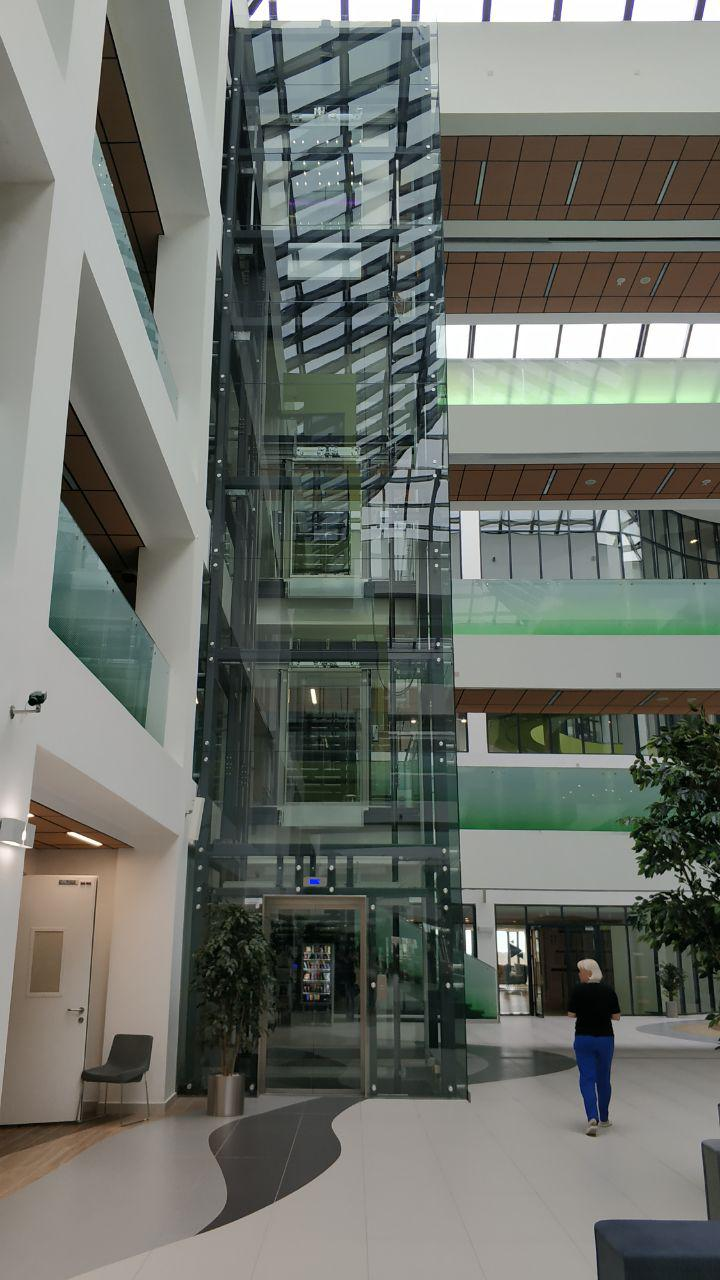
\includegraphics[width=5cm]{history/info/fintex/i3}
        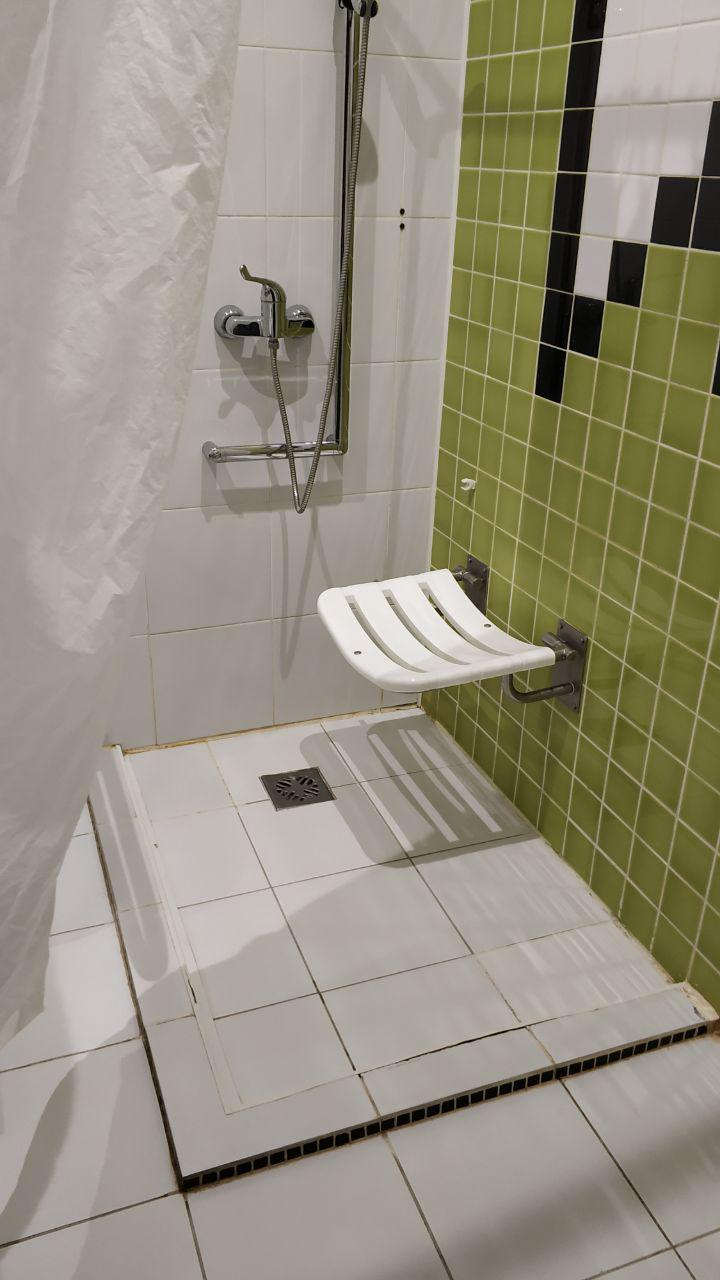
\includegraphics[width=5cm]{history/info/fintex/i4}
    \end{center}
\end{figure}

\section*{Подготовка участников}

Для вовлечения участников в олимпиаду были разработаны «Урок НТИ» и «Демо-этап» олимпиады, благодаря чему участники могли определиться с выбором профилей и попробовать свои силы.

«Урок НТИ» (\url{http://nti-contest.ru/ntilessonteacher/}) – это инициатива Олимпиады НТИ, проходившая в сентябре 2018 года и направленная на распространение информации об НТИ среди школьников и привлечение их к Олимпиаде НТИ через проведение уроков и занятий в школах и учреждениях дополнительного образования. Учебный материал для проведения «Урока НТИ» сформирован в виде конструктора, с помощью которого учителя могли собрать урок по теме НТИ. Урок позволяет познакомить учащихся НТИ и  с профилями Олимпиады НТИ, организовать практическую работу по решению задач в рамках выбранного профиля. Для участия в проекте «Урок НТИ» зарегистрировалось 2185 педагогов.

Демо-этап Олимпиады НТИ (\url{https://stepik.org/course/24389/syllabus}) – это публикация задач олимпиады в открытом доступе. Демо-этап создан для знакомства с задачами по профилям олимпиады, тренировки и испытания собственных знаний и умений решать непростые инженерные задачи.  Прежде чем определиться с участием в олимпиаде и выбором профиля,  потенциальные участники и их наставники могут познакомиться с задачами и выбрать наиболее интересный для себя профиль.

Чтобы участники могли восполнить недостаток практических компетенций и изучить оборудование, на котором им предстоит работать на заключительном этапе Олимпиады НТИ, разработчики направлений представляют методические материалы для самостоятельной практики и самоподготовки, проводят вебинары для участников и педагогов с ответами на вопросы и подбирают подготовительные курсы, совместно с площадками подготовки проводят хакатоны для участников с возможностью попробовать на практике фрагменты финальной задачи. 

Команды разработчиков профилей с целью эффективной подготовки к Олимпиаде НТИ создали видео разборы задач 2 этапа, которые доступны на канале Олимпиады НТИ, \url{https://www.youtube.com/channel/UCZV1CNpOrDNj7tuWuf35lgw/playlists} в 2018 году разработан курс (веб-сайт: \url{https://stepik.org/course/15697/syllabus}) по подготовке школьников к Олимпиаде НТИ на основе контента олимпиады 2017/2018 учебного года. Курс содержит задачи предметных треков 1 и 3 этапа по предметам: математика, физика, информатика, химия и биология и задачи 2 этапа по профилям олимпиады. Курс может использоваться наставниками и самими участниками для подготовки к олимпиаде следующего года. Формат курса максимально приближает участников к реальным условиям олимпиады.

Все указанные материалы находятся в свободном доступе и размещены на официальном сайте олимпиады, на страницах профилей в разделе «Материалы для участников». 

Материалы по профилю «Программная инженерия финансовых технологий»: \url{http://nti-contest.ru/profiles/fintech/}

Олимпиада НТИ является промежуточным итогом работы по реализации дорожной карты НТИ «Кружковое движение»: подготовка к ней велась в фаблабах, ЦМИТах, детских технопарках, на базе активных школ и лицеев, центров дополнительного образования по всей России. Рабочая группа «Кружковое движение» НТИ направлена на развитие технологического сообщества, объединяющего школьников и студентов, ориентированных на инженерную деятельность на рынках НТИ, самодеятельных технических энтузиастов, лидеров технологических кружков, разработчиков педагогических технологий, технологических предпринимателей, популяризаторов науки и технологий.

\section*{Популяризация Олимпиады НТИ}

Олимпиада НТИ широко освещается в различных средствах массовой информации (телевидение, печатные издания, электронные издания). В период с 15 августа 2018 года (начало подготовки к регистрациям) до 3 апреля 2019 года, по данным Медиалогии, Олимпиада НТИ упоминалась в СМИ 2 301 раз, из них 633 раза на федеральном уровне, 1655 на региональном уровне, 13 на зарубежном уровне. 

Во время проведения отборочных этапов Олимпиада НТИ освещалась в федеральных, массовых, родительских, образовательных и иных медиа («ИТАР-ТАСС», «РИА-Новости», «Интерфакс», «Такие Дела», «Летидор», «Дети.Мэйл.ру», «Индикатор», «Занимательная робототехника», «Чердак.Ру», «Habrahabr», «Rusbase», \linebreak «Учёба.Ру»), официальных образовательных порталах и порталах органов государственности власти в регионах  (Новосибирск, Санкт-Петербург, Великий Новгород, Иннополис, Томск, Владивосток, Калининград, Тюмень, Курск, Курган, Тамбов, Мурманск, Новогород, Вологда и т.д.), в печатных изданиях («Российская газета», «Известия»). Радио «Медиаметрикс», программа «Выбор Родителей» под руководством автора самого большого блога для родителей в России.  Кампания по привлечению шла также в научно-популярных группах и группах вузов и площадок партнеров (МАИ, НГУ, Абитуриент НГУ,  ДВФУ, Школьники ДВФУ, Абитуриенты ДВФУ, Мурманский Арктический государственный университет, СибГУ им. М.Ф. Решетнева, Кванториум, АНО ДТ Красноярский кванториум,  НовГУ, ТПУ, абитуриенты ТПУ, МГППУ, Московский Политех, школа Летово, технопарк Академгородка, Сколтех, Иннополис, группы довузовского управления университета Иннополис, Политех Петра, ИТМО, ИРНИТУ, студенты ИРНИТУ, АУ УР РЦИиОКО, Детский технопарк INGENERIKA, Инкубатор Профи, Центр компетенций для детей Поколение 2035, Лаборатория НГУ Инжевика, Чеченский государственный университет, Айти школа Орбита, Фонд Книту, Фонд Золотое сечение, ЦМИТЫ Коптер, Ноосфера, Рекорд, Уникум, Stem-Байкал, Роболатория, Академия Технолаб, Образовательный проект для подростков Tula Teens ,  Проектория, ЯКласс, Фаблаб Политех и другие).  Заключительный этап Олимпиады НТИ в 2018/2019 учебном году проходил при участии журналистов таких печатных изданий, как «Российская газета», «Известия»; федеральных телевизионных каналов («Россия 24» (6 репортажей), «Общественное телевидение России»), федеральных новостных агентств («РИА-Новости», «ИТАР-ТАСС», «Интерфакс») научно-популярных порталов  «Rusbase», «Habrahabr», «Индикатор», «Такие Дела», радиостанций («Радио России», «МедиаМетрикс») Профильные издания освещали соответствующие направления Олимпиады НТИ («Крылья Родины» – «Беспилотные авиационные системы»). В ходе финалов Олимпиады НТИ были инициированы события, вызывающие дополнительный интерес как со стороны участников, так и со стороны СМИ. Так, например в рамках финала в Новосибирском государственном университете, участники встретились с Нобелевским лауреатом Хироси Амано, информация об этом событии была распространена ведущими федеральными агентствами и телеканалами. Разработка победителей профиля «Нейротехнологии», привлекла внимание известной актрисы Екатерины Варнавы, которая написала о своих впечатлениях в блоге с аудиторией 5 млн. 400 тысяч человек, позитивную реакцию на ее пост о победителях олимпиады продемонстрировали больше 75 тысяч пользователей. 

Широкое освещение мероприятий заключительного этапа имеет своей целью распространение информации среди потенциальных участников Олимпиады НТИ будущего года – учеников 7-11 классов и направлено на привлечение талантливых школьников со всей России и активное участие их родителей. В минувшем году была проведена большая работа с целевой аудиторией родителей, чьи дети учатся в 7-11 классах (появилась собственная передача «Выше среднего» на радио Медиаметрикс, регулярно выходят материалы на портале для активных родителей «Летидор», были инициированы эфиры в передача автора самого большого блога для родителей в России (1,6 млн.человек). 

Для привлечения внимания участников к конкретным профилям Олимпиады НТИ ведется точечная работа по освещению их разработок и задач. Инициированы эфиры на радио «Медиаметрикс», тексты в таких медиа как «Rusbase», «Понедельник», «Executive», «БОСС».

В отдельное направление выделена работа с финалистами Олимпиады НТИ с особенными достижениями. Регулярно, а не только в период проведения финалов, инициируются и выходят публикации в таких медиа как: «Российская Газета», «Известия», «Такие Дела», «Индикатор», «RusBase», «Летидор», «Дети Мэйл ру», радио «Медиаметрикс», запущен сервис подкасты в социальной сети ВК, его героями становятся как финалисты, так и разработчики профилей, партнеры, учредители и организаторы Олимпиады НТИ. 
Список лучших материалов об Олимпиаде: \url{http://nti-contest.ru/publications/}.

\chapter{Профиль <<Программная
инженерия финансовых технологий>>}

Профиль для Олимпиады НТИ 2018-2019 учебного года ''Программная
инженерия финансовых технологий'' знакомил школьников с подходами,
использующимися для биометрической идентификации человека по лицу. А
поскольку задачи, лежащие перед специалистами в финансовом секторе
гораздо шире, то начиная со второго отборочного этапа участники
профиля знакомились не только математическими и алгоритмическими
основами технологий сбора, обработки и анализа биометрической
информации с помощью изображений, обеспечения безопасности при
идентификации человека по лицу, но и изучали язык структурированных
запросов SQL и приемы использования технологии распределенного реестра
в качестве платежной системы. В результате учащиеся 9-11 классов,
прошедшие все этапы олимпиады демонстрировали понимание основных
операций, необходимых для создания простых приложений, использующих
биометрическую идентификацию: выделение из видео-потока, обработка и
хранение биометрической информации, идентификация человека по лицу при
схеме один из многих, защита процесса идентификации от мошенничества,
использование результатов идентификации для авторизации пользователя в
информационной системе на выполение определенных операций. Для того,
чтобы сделать это возможным в течение олимпиады проводилась цикл
образовательных и отборочных мероприятий. 

Первый отборочный дистанционный этап (индивидуальный) определял общий
уровень подготовки школьников по предметам математика и информатика. 
Решая задачи по программированию, школьники должны были
продемонстрировать простейшие навыки составления и отладки программ,
обрабатывающих  массивы данных, и понимание таких тем, как
комбинаторика, операции со строками, вычислительная геометрия, теория
графов. Задачи по математике проверяли у участников  знания по
алгебре, комбинаторике, геометрии. Количество попыток сдачи решения
задач не ограничивалось. Таким образом, задачи первого этапа выявляли
наличие у участников знаний необходимых не только для решения задач
следующего этапа, но и финальной задачи.

Логика составления задач второго отборочного этапа требовала от
участников объединения в команды, поскольку их было сложно в сроки
второго этапа решить индивидуальному участнику. Несмотря на то, что
для решения всех задач этапа необходимо было писать программы,
школьники для некоторых задач должны были изучить базовые темы из
''Линейной алгебры''. Перед решением задач командам также было
предложен набор видео-лекций ''Введение в блокчейн технологии'' и
конспект занятий по теме ''Введение в идентификацию человека с
использованием биометрических методов'', подготовленными Университетом
Иннополис. Эти и дополнительные знания позволяли во втором этапе
проводить базовую обработку изображений и видео-потока, анализ
информации с изображения, поиск изображения по заданным критериям,
определять характер изменения элементов изображения в видео-потоке, а
также продемонстрировать базовые навыки работы с реляционными базами
данных и понимание приниципов работы Ethereum-контрактов.

После второго этапа команды, прошедшие в финал профиля, участвовали в
трех дистанционных хакатонах.

\begin{itemize}
    \item В ходе первого хакатона каждый школьник индивидуально должен был
    закрепить свои навыки в написании простейшего приложения для блокчейн
    сети, технологически совместимой с блокчейн Ethereum, а именно
    подготовить программное обеспечение для выполнения функционала
    простого кошелька.
    
    \item Второй хакатон был также направлен на разработку для блокчейн
    платформы --- участникам, объединившись в команды, предлагалось
    разработать простое децентрализованное приложение - адресную книгу, в
    которой можно было бы управлять регистрациями между именами
    пользователей их Ethereum адресами. Дополнительными заданием было
    подумать над оптимизацией хранения и обработки данных так, чтобы эти
    операции потребляли минимальное количество вычислительных ресурсов.
    
    \item Перед третьим хакатоном участники должны были зарегистрироваться
    в платформе \textit{Microsoft Azure} для доступа к сервису
    \textit{Microsoft Face API}. Заданием хакатона было написать
    минимально работающее приложение для индетификации человека по лицу с
    использованием вышеперечисленного сервиса. Кадры с лицом человека
    участники должны были находить в видео-потоке.
    
\end{itemize}
    
Данные хакатоны позволили командам получить все нобходимые навыки для
решения задачи в заключительном этапе, поскольку полностью повторяли
(но в более коротком промежутке времени) процесс проведения
заключительного этапа: задания для школьников были сформулированы в
виде пользовательских историй (User Stories), в качестве хранилища
для кода решения необходимо было использовать систему ведения версий
Git, а правильность решения проверять в автоматической системе
тестирования, основанной на GitLab CI/CD.

Командная задача заключительно этапа была логическим заверешением той
работы, которую проделали участники на отборочных этапах. Школьники
должны были написать приложение для идентификации человека по лицу,
что позволяло получить пользователю доступ к платежным операциям,
реализованными на платформы Ethereum: перевод средств другому
пользователю по его номеру телефона, заранее зарегистрированному в
общем реестре адресов, получение баланса и истории переводов,
геренерация платежных чеков на предъвителя. Также в заключительный
этап входил индивидуальный тур, в ходе которого участники решали
задачи по математике и информатике. Задачи по математике покрывали
следующие области математики: оптимизация, комбинаторика, алгебра и
геометрия. А темы задач по информатике перекликались с классическими
темами всероссийской олимпиады школьников.

\part{Первый этап}

\newpage

\section*{Описание этапа}

Первый отборочный тур проводится индивидуально в сети Интернет, работы оцениваются автоматически средствами системы онлайн-тестирования.

Для каждой из параллелей (9 класс или 10-11 класс) предлагается свой набор задач по математике, задачи по информатике общие для всех участников. Решение задач по информатике предполагало написание программ. Участники не были ограничены в выборе языка программирования для решения задач. На решение задач каждого предмета первого отборочного этапа участникам давалось 2 дня. У участников было три временных слота по 2 дня каждый, когда они могли решать задачи по предмету. Решение каждой задачи дает определенное количество баллов.

Участники получают оценку за решение задач в совокупности по всем предметам данного профиля (математика и информатика) --- суммарно от 0 до 200 баллов.
  
\chapter{Задачи первого этапа. Математика.}

\section{Первая попытка. Задачи 9 класса.}

\subimport{1st_tour/math/try_1/}{math_try_1_9.tex}

\section{Первая попытка. Задачи 10-11 класса.}

\subimport{1st_tour/math/try_1/}{math_try_1_10_11.tex}

\section{Вторая попытка. Задачи 9 класса.}

\subimport{1st_tour/math/try_2/}{math_try_2_9.tex}

\section{Вторая попытка. Задачи 10-11 класса.}

\subimport{1st_tour/math/try_2/}{math_try_2_10_11.tex}

\section{Третья попытка. Задачи 9 класса.}

\subimport{1st_tour/math/try_3/}{math_try_3_9.tex}

\section{Третья попытка. Задачи 10-11 класса.}

\subimport{1st_tour/math/try_3/}{math_try_3_10_11.tex}

\chapter{Задачи первого этапа. Углубленная информатика.}

\section{Первая попытка.}

\subimport{1st_tour/inf2/try_1/}{inf2_try_1.tex}

\section{Вторая попытка.}

\subimport{1st_tour/inf2/try_2/}{inf2_try_2.tex}

\section{Третья попытка.}

\subimport{1st_tour/inf2/try_3/}{inf2_try_3.tex}
 
\part{Второй этап}
\newpage

\section*{Описание этапа}

Второй отборочный этап проводится в командном формате в сети Интернет, работы оцениваются автоматически средствами системы онлайн-тестирования.

Продолжительность второго этапа составляет 52 дня. Задачи требуют от участников наличие навыков программирования, носят междисциплинарный характер и помогают отработать те навыки, которые потребуются для решения командной задачи заключительного этапа.

Участники не были ограничены в выборе языка программирования для решения задач.

Объем и сложность задач этого этапа подобраны таким образом, чтобы решение всех задач одним человеком было маловероятно. Это призвано обеспечить включение командной работы и распределения обязанностей. Решение каждой задачи дает определенное количество баллов. В части задач баллы зачисляются в полном объеме за правильное решение задачи, в другой части задач баллы начислялись за частичное решени. В данном этапе можно получить суммарно от 0 до 105 баллов.

Задачи выкладывались партиями: в начале второго этапа и затем через каждую неделю.

Команды могут выполнять задачи в любом порядке. Задачи допускают неограниченное число попыток сдать решение.

\clearpage
\chapter{Задачи второго этапа}
\chapter{Финансовые технологии.}

\section{Блок задач 1.}

\subimport{2nd_tour/fintex/task_01/}{statement}
\subimport{2nd_tour/fintex/task_02/}{statement}
\subimport{2nd_tour/fintex/task_03/}{statement}
\subimport{2nd_tour/fintex/task_04/}{statement}

\section{Блок задач 2.}

\subimport{2nd_tour/fintex/task_05/}{statement}
\subimport{2nd_tour/fintex/task_06/}{statement}

\section{Блок задач 3.}

\subimport{2nd_tour/fintex/task_07/}{statement}
\subimport{2nd_tour/fintex/task_08/}{statement}
\subimport{2nd_tour/fintex/task_09/}{statement}

\section{Блок задач 4.}

\subimport{2nd_tour/fintex/task_10/}{statement}
\subimport{2nd_tour/fintex/task_11/}{statement}

\section{Блок задач 5.}

\subimport{2nd_tour/fintex/task_12/}{statement}
\subimport{2nd_tour/fintex/task_13/}{statement}


\part{Заключительный этап}
 
\clearpage
\chapter{Предметный тур}

На индивидуальное решение задач дается по 2 часа на один предмет.
Для каждой из параллелей (9 класс или 10-11 класс) предлагается свой
набор задач по математике, задачи по информатике - общие для всех
участников.

Решение каждой задачи по математике дает определенное количество
баллов (см. критерии оценки). При этом некоторые задачи делятся на
подзадачи. За каждую подзадачу можно получить от 0 до указанного
количества баллов.

Решение задач по информатике предполагало написание программ.
Ограничения по используемым языкам программирования не было.
Проверочные тесты для каждой задачи по информатике делились на
несколько групп. Прохождение всех тестов в группе тестов дает
определенное количество баллов за решение задачи.

Участники получают оценку за решение задач в совокупности по
всем предметам данного профиля (математика и информатика) ---
суммарно от 0 до 200 баллов:

\begin{itemize}
    \item {\bf Математика 9 класс} количество набранных баллов
    (от 0 до 100);
    \item {\bf Математика 10-11 класс} количество набранных баллов
    (от 0 до 100);
    \item {\bf Информатика} количество набранных баллов (от 0 до
    300) делится на коэффициент 3.
\end{itemize}


\section{Математика. 9 класс}

\subimport{final/subject_tour/math0903_irs_9/task_01/}{statement}
\subimport{final/subject_tour/math0903_irs_9/task_01/}{solution}

\subimport{final/subject_tour/math0903_irs_9/task_02/}{statement}
\subimport{final/subject_tour/math0903_irs_9/task_02/}{solution}

\subimport{final/subject_tour/math0903_irs_9/task_03/}{statement}
\subimport{final/subject_tour/math0903_irs_9/task_03/}{solution}


\section{Математика. 10-11 класс}

\subimport{final/subject_tour/math0903_irs_10/task_01/}{statement}
\subimport{final/subject_tour/math0903_irs_10/task_01/}{solution}

\subimport{final/subject_tour/math0903_irs_10/task_02/}{statement}
\subimport{final/subject_tour/math0903_irs_10/task_02/}{solution}

\subimport{final/subject_tour/math0903_irs_10/task_03/}{statement}
\subimport{final/subject_tour/math0903_irs_10/task_03/}{solution}


\section{Информатика}

\subimport{final/subject_tour/inf0903_irs/task_01/}{statement.tex}
\subimport{final/subject_tour/inf0903_irs/task_02/}{statement.tex}
\subimport{final/subject_tour/inf0903_irs/task_03/}{statement.tex}


\chapter{Командный тур}

\section{Легенда}
Современные банки в погоне за привлечением клиентов разрабатывают и вводят в
эксплуатацию все более комфортные сервисы. 

\twoitems{Например, российские банки Сбербанк и
Тинькофф-банк вводят в строй банкоматы, способные идентифицировать человека по 
лицу}{\url{https://tass.ru/ekonomika/4402287}}
{\url{https://www.banki.ru/news/lenta/?id=10740603}}

Банк ''Ак Барс'' планирует использовать технологию \textit{Face2Pay} в
образовательных учреждениях для оплаты школьниками питания:
\url{https://tass.ru/ekonomika/5607346}.

Не только в России (\url{https://www.banki.ru/news/lenta/?id=10670764}), но и в других
странах мира (\url{https://www.vesti.ru/doc.html?id=3126288}) разрабатываются системы
для оплаты общественного транспорта с помощью технологий распознавания человека по лицу.

Также стремясь увеличить скорость перемещения денежных средств (в частности для
межбанковских и международных переводов) банки рассматривают альтернативные платежные
системы, основанные на технологии блокчейн:
\begin{itemize}
  \item \url{https://www.jpmorgan.com/global/news/digital-coin-payments}
  \item \url{http://coinlog.ru/6-mirovyh-bankov-zapuskayut-stejblkoiny-v-obshhej-blokchejn-seti-ibm/}
  \item \url{https://bits.media/pyat-bankov-yaponii-obedinilis-dlya-sozdaniya-blokcheyn-resheniy/}
  \item \url{https://cryptoratings.ru/news/alfa-bank-podklyuchilsya-k-blokchejn-seti-marco-polo/}
\end{itemize}

Поскольку перечисленные выше технологии становятся трендом в современном финансовом
секторе, то участниками профиля ''Программная инженерия финансовых технологий''
предлагается разработать прототип программного обеспечения банкомата, проводящего операции
в блокчейн сети, и идентифицирующего пользователя по лицу.

При этом разработка модели машинного обучения для распознавания и идентификации человека по лицу
остается за рамками данного прототипа. Как и в реальных индустриальных проектах, на стадии
прототипа вместо разработки собственной модели будет применяться уже готовое решение, а именно
сервис \textit{Microsoft Face API}, наиболее удовлетворяющий нужды данного проекта.

В общих чертах работа банкомата описывается следующим образом:
\begin{itemize}
  \item Пользователь идентифицируется банкоматом по лицу.
  \item В качестве дополнительной меры безопасности банкомат может запросить от пользователя выполнить определенные действия, для проверки, что перед камерой банкомата не ''плоское'' изображение пользователя и не маникен.
  \item Поскольку блокчейн сеть авторизует пользовательские операции посредством приватного ключа пользователя, ключ генерируется на основании идентификатора пользователя, возвращенного сервисом идентификации человека по лицу, и PIN-кодом, введенным человеком. Таким образом, происходит защита от перехвата индентификатора человека.
  \item После получения приватного ключа возможны операции получения баланса, проведение платежей, получения истории платежей.
  \item Платежи другим пользователям осуществляются по их номеру телефона  
\end{itemize}

Следовательно, чтобы ПО банкомата могло работать необходимо реализовать дополнительные сервисные функции, осуществляемые при регистрации нового пользователя в систему (например, в офисе банка):
\begin{itemize}
  \item Управление пользователями в сервисе распознования по лицу: добавление и удаление пользователя и изображений его лица.
  \item Управление соответствями между пользователем и его номером телефона: регистрация и удаление соответствия.
  \item Для избежания мошенничеств регистрация и удаление соответствия должны подтверждаться авторизованным лицом (администратором в банке).
\end{itemize}


\section{Набор заданий}
Решение командной задачи разбито на подзадачи, сгруппированные в 3 набора.

Каждая подзадача (\textit{user story}) формулирует необходимый функционал,
который должен быть реализован командой, а также набор приемочных
тестов (\textit{acceptance criteria}), позволяющих проверить в полном ли
объеме решена данная подзадача.

Каждый набор подзадач предлагается решать в отдельном этапе (\textit{итерации}).
Подзадачи в первом наборе позволяют школьникам продемонстрировать базовое понимание
принципов решения данной задачи. Они могут быть решены с использованием тех разработок,
котороые были реализованы участниками финала на учебно-тренировочных сборах.
Поздадачи второй итерации позволяют реализовать минимально рабочий продукт.
Третья итерация состоит из подзадач повышенной сложности, которые требуют от
старшеклассников продемонстрировать более глубокое понимание принципов написания
контрактов для сети блокчейн, а также использовать знания из олимпиады по
программированию для оптимизации работы с видео-потоком.

На каждом этапе решение подзадач проверялось с помощью системы автоматической
системы оценивания, которая запускала решение участников с теми или иными
параметрами в соответствии с приемочными тестами. 

\subsection*{Первая итерация}

Участникам необходимо разработать базовый функционал для скриптов \texttt{setup.py}, 
\texttt{face-management.py} и \texttt{faceid.py}, реализовать соответствующие
Ethereum-контракты, тем самым решая следующие подзадачи:

\footnotesize
\begin{center}
\begin{tabular}{ |l|c|  }
 \hline
  \thead{user story (*)} & \thead{acceptance \\ criteria} \\
 \hline

US-001 Регистрация контракта & все \\
US-004 Простое добавление пользователя в сервис индентификации & все \\
US-013 Получение баланса идентифицированного пользователя & все \\

 \hline
\end{tabular}
\end{center}
\begin{flushright}
\textit{(*) формулировки задач приведены в разделе ''Подробное описание подзадач''.}
\end{flushright}
\normalsize

Решение подзадач было направлено на проверку следующих компетенций:
\begin{itemize}
    \item инициализация аккаунтов тестовой публичной сети Ethereum для тестирования
    решения в ходе процесса разработки;
    \item настройка окружения разработки программного обеспечения для использования
    системы ведения версий \textit{Git}, Python-библиотек для взаимодействия с
    узлами блокчейн платформы Ethereum и \textit{Microsoft Face API};
    \item написание и отладка программ на языке Python, работающих с параметрами
    командной строки;
    \item обеспечение отправки JSON-RPC запросов (платежные операции) из программ
    на языке Python к провайдерам \texttt{Web3};
    \item написание и отладка Ethereum контрактов на языке Solidity;
    \item подготовка тестовых данных --- видео-файлов для работы с сервисом
    распознавания человека по лицу;
    \item получение отдельных кадров из видео-потока; 
    \item обеспечение отправки REST запросов к сервису \textit{Microsoft Face API}
    из программ на языке Python.
\end{itemize}

\subsection*{Вторая итерация}

Участникам необходимо завершить работу над минимально достаточным прототипом
программного обеспечения банкомата, который бы позволял
\begin{itemize}
    \item идентифицировать человека по лицу;
    \item управлять соответствиями между аккаунтом пользователя и его телефонным номером;
    \item отправлять средства другому зарегистрированному в системе пользователю.
\end{itemize}
Данный функционал покрывался следующими подзадачами:

\footnotesize
\begin{center}
\begin{tabular}{ |l|c|  }
 \hline
  \thead{user story (*)} & \thead{acceptance \\ criteria} \\
 \hline

US-002 Вывод владельца контракта регистра соответствий & все \\
US-003 Изменение владельца контракта регистра соответствий & все \\
US-006 Получение всех пользователей из сервиса идентификации & все \\
US-007 Удаление пользователя из сервиса идентификации & все \\
US-008 Запуск обучения сервиса индентификации & \makecell{все, кроме \\ AC-008-04} \\
US-010 Идентификация пользователя & \makecell{все, кроме \\ AC-010-04} \\
US-014 Отправка запроса на регистрацию соответствия & все \\
US-015 Отправка запроса на удаление соответствия & все \\
US-016 Отмена запроса на регистрацию или удаление соответствия & все \\
US-017 Отправка средств & все \\
US-021 Получение истории платежей & все \\
US-023 Получение всех запросов на регистрацию соответствий & все \\
US-024 Получение всех запросов на удаление соответствий & все \\
US-025 Подтверждение запросов на регистрацию или удаление соответствий & все \\
US-026 Получение аккаунта по номеру телефона & все \\

 \hline
\end{tabular}
\end{center}
\begin{flushright}
\textit{(*) формулировки задач приведены в разделе ''Подробное описание подзадач''.}
\end{flushright}
\normalsize

Решение подзадач было направлено на проверку следующих компетенций:
\begin{itemize}
    \item взаимодействие с сервисом распознавания человека по лицу для наполнения
    его необходимыми данными, обучения и выполнения операций распознавания; 
    \item разработка контракта с простейшей моделью разграничения доступа;
    \item разработка схемы взаимодействия структур данных для контракта с
    заданными характеристиками;
    \item обеспечение отправки JSON-RPC запросов (транзакции на вызов методов
    Ethereum контрактов, получение данных из блокчейн сети) из программ на языке Python
    к провайдерам \texttt{Web3};
    \item выстраивание процесса интеграционного тестирования компонент приложения,
    работающего с сервисом распознавания лица и узлами блокчейн сети.
\end{itemize}

\subsection*{Третья итерация}

Работа участников должна быть направлена на наращивание функционала прототипа
программного обеспечения банкомата. В ходе третьей итерации должна была появиться
защита от мошенничества при операциях распознавания по лицу и возможность
формировать отложенные платежи.
После заверешения итерации у участников должно быть 3 Python-скрипта и
2 Ethereum-контракта, закрывающие последнии набор подзадач:

\footnotesize
\begin{center}
\begin{tabular}{ |l|  }
 \hline
  \thead{user story (*), все acceptance criteria} \\
 \hline

US-005 Улучшенное добавление пользователя в сервис индентификации \\
US-008 Запуск обучения сервиса индентификации \\
US-009 Обнаружение уже добавленного пользователя \\
US-010 Идентификация пользователя \\
US-011 Запрос действий на безопасную идентификацию пользователя \\
US-012 Безопасная идентификация пользователя \\
US-018 Генерация сертификата на получение средств \\
US-019 Использование сертификата на получение средств \\
US-020 Вернуть средства из неиспользованных сертификатов \\
US-022 Получение истории платежей, включая использование сертификатов \\

 \hline
\end{tabular}
\end{center}
\begin{flushright}
\textit{(*) формулировки задач приведены в разделе ''Подробное описание подзадач''.}
\end{flushright}
\normalsize

Решение подзадач было направлено на проверку следующих компетенций:
\begin{itemize}
    \item оптимизация работы c видео-потоком для уменьшения количества
    обрабатываемых кадров;
    \item проверки истинности информации с использованием цифровой подписи.
\end{itemize}



\section{Условия проведения}
\begin{itemize}
    \item В первые день соревнований все члены команд получают ноутбук со следующим набором
    установленного программного обеспечения:
    \begin{itemize}
        \item набор Python инструментария Anaconda c установленными библиотеками \texttt{web3} (\texttt{v5.0.0a3}), \texttt{cognitive\_face}, \texttt{opencv-python};
        \item среды разработки PyCharm и WingIDE;
        \item компилятор языка Solidity \texttt{solc} (\texttt{v0.5.4});
        \item клиент системы ведения версий \texttt{git};
        \item Интернет-браузер Chrome.
    \end{itemize}
    Каждый ноутбук имеет возможность выхода в сеть Интернет. Команды могут использовать
    собственные ноутбуки.

    \item Команды могут устанавливать дополнительное программное обеспечение, но после
    согласования с членами жюри.

    \item Участники во время командного этапа финального тура могут использовать интернет
    и заранее подготовленные библиотеки для решения задачи.

    \item Участники должны использовать язык программирования Python для написания
    программ, использующих командную строку. Для написания Ethereum контрактов
    участники могут использовать любой язык программирования.

    \item Для работы с сервисом \textit{Microsoft Face API} участникам предоставляется
    один ключ подписки на команду, а также базовый URL для доступа к REST API. При
    доступе к сервису с помощью данного ключа действует ограничение на 10 запросов в
    секунду. Участники одной команды должны сами заботиться о том, чтобы держать ключ
    в тайне от других команд. Ключ не должен передаваться третьим лицам. Если ресурс
    ключа подписки (примерно 60000 запросов) полностью используется командой, то
    организаторы вправе не предоставлять команде другой ключ.

    \item Участники не могут использовать помощь тренера, сопровождающего лица или
    привлекать третьих лиц для решения задачи.

    \item Финальная задача формулируется участникам в первый день финального тура,
    но участники выполняют решение  задачи поэтапно. Критерии прохождения каждого
    этапа формулируются для каждого дня финального тура. За подзадачи, решенные в
    конкретном этапе начисляются, баллы. Баллы за подзадачи можно получить только
    в день, закрепленный за конкретным этапом.

    \item В начале первого дня состязаний участники каждой команды получают доступ 
    к репозиторию на серверах GitLab.com. Каждая команда имеет свой собственный 
    репозиторий. Члены других команд не имеют доступ к чужим репозиториям.

    \item В течение дня не ведется учет количества изменений, которые команды
    регистрируют в Git-репозитории.

    \item В конце каждого дня финального этапа жюри проверяет решение участников
    на соответствие приемочным тестам для каждой подзадачи, входящей в набор
    для соответствующей итерации.

    \item Баллы за все подзадачи, для которых прошло приемочное тестирование,
    определяют баллы, набранные командой в данный день соревнований.

    \item Система автоматического тестирования имеет следующую конфигурацию:
    \begin{itemize}
        \item OS Linux
        \item Python \texttt{v3.6}
        \item Python модули (перечислены) и соответствующие зависимости
        (не перечислены): \texttt{web3} (\texttt{v5.0.0a3}), \texttt{opencv-python}, 
        \texttt{cognitive\_face}, \texttt{dlib},  \texttt{imutils}, 
        \texttt{ethereum}
        \item \texttt{/usr/local/bin/solc} (\texttt{v0.5.4})
        \item \texttt{/opt/shape\_predictor\_68\_face\_landmarks.dat}
    \end{itemize}

    \item После выставления баллов, командам предоставляется доступ к системе
    автоматического тестирования, ответственной за проведение приемочных тестов в
    конкретный день состязаний, так что члены команды могут ознакомиться с 
    логикой проверки и подать апелляцию, если не согласны с корректностью проведения
    тестов.

    \item После рассмотрения сути апелляции, жюри вправе провести тестирование
    вручную и назначить команде баллы за соответствующие подзадачи.

    \item В начале следующего дня состязаний жюри выдает всем командам свое решение
    подзадач предыдущего дня, которое команды могут использовать для того, чтобы
    решать следующий набор подзадач.

    \item Описанные выше условия могут быть изменены членами жюри. Все изменения в
    условиях объявляются участникам перед началом каждого дня состязаний.
\end{itemize}

\section{Процедура проведения приемочного тестирования и критерии оценки}
Для каждого дня соревнований (для каждой итерации) справедлива следующая процедура
приемочного тестирования:
\begin{itemize}
    \item В конце каждого дня финального этапа команды должны сформировать запрос
    на слияние (\textit{Merge Request}) из своей ветки исходного кода в основную ветку
    (\textit{master}) в Git-репозитории.
    \item Команда ответственна за то, чтобы в запросе на слияние не должно быть
    конфликтов. Запрос на слияние с конфликтами может не рассматриваться жюри для
    выполнения приемочного тестирования.
    \item После того, как все команды отправили запросы на слияние, жюри одобряет
    все запросы и приступает к приемочному тестированию, для тех подзадач, которые
    входят в соответствующую итерацию. Для этого исходный код приложения команды
    загружается в систему автоматического тестирования (поддержка которой осуществляется
    функциональность GitLab CI/CD), где запускаются автоматические тесты на соответствие
    решения участников требованиям к приемочным тестам (\textit{acceptance criteria}).
    \item Если все приемочные тесты для данной подзадачи пройдены успешно,
    команда получает баллы за данную подзадачу. Если хотя бы один тест не проходит,
    то баллы за данное подзадачу не начисляются.
\end{itemize}

Приемочные тесты для каждой подзадачи описаны в разделе ''Подробное описание подзадач''.

Дальше перечислены баллы, которые получает команда за решение подзадач в каждой итерации.

Максимальное количество баллов, которое может набрать команда за решение всех 
подзадач --- 400. 

\subsection*{Первая итерация}

\footnotesize
\begin{center}
\begin{tabular}{ |l|c|  }
 \hline
  \thead{user story} & \thead{баллы} \\
 \hline

US-001 Регистрация контракта & 10 \\
US-004 Простое добавление пользователя в сервис индентификации & 20 \\
US-013 Получение баланса идентифицированного пользователя & 10 \\

 \hline
\end{tabular}
\end{center}
\normalsize

Максимальное количество баллов за итерацию --- 40.

\subsection*{Вторая итерация}

\footnotesize
\begin{center}
\begin{tabular}{ |l|c|  }
 \hline
  \thead{user story} & \thead{баллы} \\
 \hline

US-002 Вывод владельца контракта регистра соответствий & 10 \\
US-003 Изменение владельца контракта регистра соответствий & 10 \\
US-006 Получение всех пользователей из сервиса идентификации & 10 \\
US-007 Удаление пользователя из сервиса идентификации & 10 \\
US-008 Запуск обучения сервиса индентификации (кроме AC-008-04) & 18 \\
US-010 Идентификация пользователя (кроме AC-010-04) & 23 \\
US-014 Отправка запроса на регистрацию соответствия & 10 \\
US-015 Отправка запроса на удаление соответствия & 10 \\
US-016 Отмена запроса на регистрацию или удаление соответствия & 15 \\
US-017 Отправка средств & 10 \\
US-021 Получение истории платежей & 20 \\
US-023 Получение всех запросов на регистрацию соответствий & 10 \\
US-024 Получение всех запросов на удаление соответствий & 10 \\
US-025 Подтверждение запросов на регистрацию или удаление соответствий & 15 \\
US-026 Получение аккаунта по номеру телефона & 10 \\

 \hline
\end{tabular}
\end{center}
\normalsize

Максимальное количество баллов за итерацию --- 191.

\subsection*{Третья итерация}

\footnotesize
\begin{center}
\begin{tabular}{ |l|c|  }
 \hline
  \thead{user story} & \thead{баллы} \\
 \hline

US-005 Улучшенное добавление пользователя в сервис индентификации & 50 \\
US-008 Запуск обучения сервиса индентификации (полностью) & 2 \\
US-009 Обнаружение уже добавленного пользователя & 20 \\
US-010 Идентификация пользователя (полностью) & 2 \\
US-011 Запрос действий на безопасную идентификацию пользователя & 5 \\
US-012 Безопасная идентификация пользователя & 35 \\
US-018 Генерация сертификата на получение средств & 10 \\
US-019 Использование сертификата на получение средств & 15 \\
US-020 Вернуть средства из неиспользованных сертификатов & 20 \\
US-022 Получение истории платежей, включая использование сертификатов & 10 \\

 \hline
\end{tabular}
\end{center}
\normalsize

Максимальное количество баллов за итерацию --- 169.

\subsection*{Критерии определения команды-победителя командного тура}

\begin{itemize}
    \item Сумма баллов, набранных за решения подзадач командного тура финального этапа, определяет итоговую результативность команды (измеряемую в баллах).
    \item Команды ранжируются по результативности.
    \item Команда победитель определяется, как команда с максимальной результативностью.
\end{itemize}


\section{Подробное описание подзадач}
Решение представляет из себя набор python скриптов (компонент), каждый
из который ответственен за определенный функционал. 

Управление скриптами происходит через параметры командной строки и
через конфигурационные файлы. Параметры командной строки описываются 
тдельно в разделах, где описывается функциональность каждого скрипта.

\twoitems{Конфигурационные файлы - файлы в формате JSON, должны читаться
из текущей директории, где происходит вызов скрипта и могут быть двух типов}
{конфигурационный файл с настройками для работы с \textit{Microsoft Face API}}
{конфигурационный файл с настройками для работы с Ethereum узлом}

\subsubsection*{Конфигурационный файл с настройками для MS Face API}

Имя: \texttt{faceapi.json}

\threeitems{Содержит следующую информацию}
{\texttt{key} --- ключ подписки для использования сервиса}
{\texttt{serviceUrl} --- URL для доступа к сервису}
{\texttt{groupId} -- группа пользователей (в терминах \textit{MS Face API}),
с которой работает в данный момент скрипт}

Пример файла:
\begin{minted}[fontsize=\footnotesize]{json}
{"key": "563879b61984550e40cbbe8d3039523c",
 "serviceUrl": "https://westeurope.api.cognitive.microsoft.com/face/v1.0/",
 "groupId": "fintech-01"}
\end{minted}

\subsubsection*{Конфигурационный файл с настройками для работы с узлом Ethereum}

Имя: \texttt{network.json}

Содержит следующую информацию:
\begin{itemize}
  \item \texttt{rpcUrl} --- URL для доступа к узлу по JSON RPC;
  
  \item \texttt{privKey} --- приватный ключ аккаунта для подписи транзакций,
  отправляемых на узел Ethereum, и для локальных вызовов;
  
  \item \texttt{gasPriceUrl} --- URL для доступа к сервису, предоставляющему
  цену за газ. Данный сервис возвращает JSON, из которого нужно взять
  значение (в \textit{gwei}) из поля \texttt{fast}:
    \begin{minted}[fontsize=\footnotesize]{json}
{"block_time":19.91, "fast":10.0, "instant":25.0, "block_number":7240426,
 "standard":5.0, "health":true, "slow":3.0}
    \end{minted}
  
  \item \texttt{defaultGasPrice} --- цена за газ в wei, использующаяся,
  если нельзя получить цену за газ из сервиса.

\end{itemize}

Пример файла:
\begin{minted}[fontsize=\footnotesize]{json}
{"rpcUrl": "https://sokol.poa.network", 
 "privKey": "c5d2460186f7233c927e7db2dcc703c0e500b653ca82273b7bfad8045d85a470", 
 "gasPriceUrl": "https://gasprice.poa.network/", 
 "defaultGasPrice": 2000000000}
\end{minted}

Если это явно не прописано в описании функционала соответствующей компоненты,
она не должна оставлять после себя никаких файлов-данных. Аналогично с
получением данных - чтение данных из файла должно происходить только в
нескольких случаях:
\begin{itemize}
  \item для получения настроек для работы с \textit{MS Face API};
  
  \item для получения видеопотока, эмулирующего камеру;
  
  \item для получения настроек для работы с Ethereum узлом;
  
  \item для получения Application Binary Interface контракта или его байткода;
  
  \item или если это явно указано в описании компоненты.

\end{itemize}
в остальных случаях данные должны быть получены из сервиса
\textit{MS Face API} или блокчейн сети. 

Все компоненты, работающие с сервисом \textit{MS Face API},
должны уметь обрабатывать ситуации, когда:
\begin{itemize}
  \item недоступно подключение к сервису (сообщение об ошибке
  \texttt{''No connection to MS Face API provider''});

  \item используется некорректный ключ подписки (сообщение об
  ошибке \texttt{''Incorrect subscription key''}).

\end{itemize}

Компоненты, отправляющие транзакции в блокчейн, должны уметь обрабатывать
ситуации, когда:
\begin{itemize}
  \item недоступно подключение к узлу Ethereum (сообщение об ошибке
  \texttt{''No connection to node''});

  \item на счету аккаунта, от чьего имени выполняется транзакция,
  недостаточно средств, чтобы покрыть все затраты по использованному
  газу (сообщение об ошибке \texttt{''No enough funds to send transaction''});

  \item транзакция может не включаться в блок продолжительное время в
  зависимости от нагрузки на сеть (сообщение об ошибке
  \texttt{''Transaction is not validated too long''}).

\end{itemize}

При возникновении данных событий в терминал должно выдаваться сообщение
понятное пользователю, а не stack trace.

Возможны также другие конфигурационные файлы, необходимые для работы
тех или иных подсистем решения. Данные файлы будут отдельно описываться
в соответствующих разделах. 

\subsection*{Настройка сервиса KYC}


Развертывание и настройка в блокечейн сети регистра соответствий аккаунтов и телефонных номеров (Know Your Customer, KYC) выполняется компанией производителем программного обеспечения (тем, кто разрабатывает данный сервис). Тоже самое относится к обработчику сертификатов на получение средств. Предполагается, что в потенциальные пользователи сервиса (пользователи, регистрирующие соответствия, владельцы платежных терминалов) могут ознакомиться с опубликованным в открытом доступе исходным кодом контрактов, принять решение на основе этого, доверять ли этому разработчику и начать пользоваться сервисом.

Фиксация контрактов в блокчейн гарантирует, что приозводитель не сможет изменить логику работы приложения позднее, т.е. условия участия в системе, с которыми ознакомились пользователи, не поменяется.

Функционал сервиса KYC должен быть доступен сразу, минуя фазы настройки, когда контракт зарегистрирован в блокчейн, но еще находится в нерабочем состоянии. Поэтому первичная настройка базовых параметров по максимуму должна выполняться вовремя инициализации контракта во время его регистрации (deploy).

\begin{myverbbox}{\scriptFile}
setup.py <command> [options]
\end{myverbbox}
\scriptTitle


%-----------------------------------------------------
%US-001
\newuserstory{Регистрация контракта}



\begin{myverbbox}[\small]{\cmdLine}
$ setup.py --deploy
\end{myverbbox}
\scriptExample{
Подключается к узлу Ethereum и регистрирует следующие контракты
\begin{itemize}
  \item регистр соответствий аккаунтов и телефонных номеров в сети блокчейн. 
  \item обработчик сертификатов на получение средств.
\end{itemize}

На терминал выводятся адреса зарегистрованных контрактов. В текущей рабочей директории создается JSON файл \texttt{registrar.json}, содержащий адреса зарегистрированных контрактов.

}

% AC-001-01
\begin{myverbbox}[\small]{\output}
$ cat registrar.json
cat: registrar.json: No such file or directory
$ setup.py --deploy
KYC Registrar: 0x00360d2b7D240Ec0643B6D819ba81A09e40E5bCd
Payment Handler: 0x95426f2bC716022fCF1dEf006dbC4bB81f5B5164
$ cat registrar.json
{"registrar": {"address": "0x00360d2b7D240Ec0643B6D819ba81A09e40E5bCd", "
startBlock": 123456}, "payments": {"address": "0x95426f2bC716022fCF1dEf00
6dbC4bB81f5B5164", "startBlock": 123457}}
\end{myverbbox}
\acceptanceCriteria{В блокчейн сеть отправляются транзакции для регистрации и первичной настройке контрактов. Транзакции успешно включены в один
или несколько блоков. Для проведения транзакции выбрана цена из значения \texttt{fast}, возвращенного сервисом \texttt{https://gasprice.poa.network}. Контракты по адресу, выведенным в терминале, созданы одной из отправленных транзакций, и могут быть просмотрены с помощью браузера блоков.
}

% AC-001-02
\begin{myverbbox}[\small]{\output}
$ cat registrar.json
{"registrar": {"address": "0x00360d2b7D240Ec0643B6D819ba81A09e40E5bCd", "
startBlock": 123456}, "payments": {"address": "0x95426f2bC716022fCF1dEf00
6dbC4bB81f5B5164", "startBlock": 123457}}
$ setup.py --deploy
KYC Registrar: 0x23B40E5bCd06D819ba81A09e0340Ec06460d2b7D
Payment Handler: 0xE797A1da01eb0F951E0E400f9343De9d17A06bac
$ cat registrar.json
{"registrar": {"address": "0x23B40E5bCd06D819ba81A09e0340Ec06460d2b7D", "
startBlock": 456123}, "payments": {"address": "0xE797A1da01eb0F951E0E400f
9343De9d17A06bac", "startBlock": 456125}}
\end{myverbbox}
\acceptanceCriteria{В блокчейн сеть отправляются транзакции для регистрации и первичной настройке контрактов. Транзакции успешно включены в один
или несколько блоков. Для проведения транзакции выбрана цена из значения \texttt{defaultGasPrice} из файла \texttt{network.json}.
}

%-----------------------------------------------------
%US-002
\newuserstory{Вывод владельца контракта регистра соответствий}



\begin{myverbbox}[\small]{\cmdLine}
$ setup.py --owner registrar
\end{myverbbox}
\scriptExample{
Подключается к узлу Ethereum и получает адрес аккаунта, имеющего полномочия выполнять действия по подверждению запросов на регистрацию и удалению соответствий аккаунтов и телефонных номеров в сети блокчейн. 

На терминал выводится адрес аккаунта.

}

% AC-002-01
\begin{myverbbox}[\small]{\output}
$ cat network.json | python -mjson.tool | grep privKey 
    "privKey": "c5d2460186f7233c927e7db2dcc703c0e500b653ca82273b7bfad8045
d85a470",
$ setup.py --deploy
KYC Registrar: 0x9FdddF5bf10c65221da0a78ADAFec1D8E9EF0A7D
Payment Handler: 0xD79A8FDB771Ea12359270aD7020bcCB328C9f5f7
$ setup.py --owner registrar
Admin account: 0x9cce34F7aB185c7ABA1b7C8140d620B4BDA941d6
\end{myverbbox}
\acceptanceCriteria{Транзакции в блокчейн сеть не отправляются.
}

% AC-002-02
\begin{myverbbox}[\small]{\output}
$ cat network.json | python -mjson.tool | grep privKey 
    "privKey": "64e604787cbf194841e7b68d7cd28786f6c9a0a3ab9f8b0a0e87cb438
7ab0107",
$ cat registrar.json
{"registrar": {"address": "0x9FdddF5bf10c65221da0a78ADAFec1D8E9EF0A7D", "
startBlock": 234156}, "payments": {"address": "0xD79A8FDB771Ea12359270aD7
020bcCB328C9f5f7", "startBlock": 451247}}
$ setup.py --owner registrar
Admin account: 0x9cce34F7aB185c7ABA1b7C8140d620B4BDA941d6
\end{myverbbox}
\acceptanceCriteria{Транзакции в блокчейн сеть не отправляются.
}

%-----------------------------------------------------
%US-003
\newuserstory{Изменение владельца контракта регистра соответствий}



\begin{myverbbox}[\small]{\cmdLine}
$ setup.py --chown registrar <address>
\end{myverbbox}
\scriptExample{
Подключается к узлу Ethereum и отправляет транзакцию на изменение аккаунта, имеющего полномочия выполнять действия по подверждению запросов на регистрацию и удалению соответствий аккаунтов и телефонных номеров в сети блокчейн. Только аккаунт, в текущее время обладающий полномочиями на выполнение вышеуказанных действий, имеет возможность производить данное изменение.

На терминал выводится адрес нового аккаунта.

}

% AC-003-01
\begin{myverbbox}[\small]{\output}
$ cat network.json | python -mjson.tool | grep privKey 
    "privKey": "c5d2460186f7233c927e7db2dcc703c0e500b653ca82273b7bfad8045
d85a470",
$ setup.py --owner registrar
Admin account: 0x9cce34F7aB185c7ABA1b7C8140d620B4BDA941d6
$ setup.py --chown registrar 0x6455f1445c72ba9460c6f6ab364d3935a0ad4559
New admin account: 0x6455F1445c72BA9460C6f6AB364d3935a0AD4559
$ setup.py --owner registrar
Admin account: 0x6455F1445c72BA9460C6f6AB364d3935a0AD4559
\end{myverbbox}
\acceptanceCriteria{В блокчейн сеть отправляется транзакция для изменения аккаунта. Транзакция успешно верифицирована и включена в блок. Для проведения транзакции выбрана цена из значения \texttt{fast}, возвращенного сервисом \texttt{https://gasprice.poa.network}.
}

% AC-003-02
\begin{myverbbox}[\small]{\output}
$ cat network.json | python -mjson.tool | grep privKey 
    "privKey": "c5d2460186f7233c927e7db2dcc703c0e500b653ca82273b7bfad8045
d85a470",
$ setup.py --owner registrar
Admin account: 0x6455F1445c72BA9460C6f6AB364d3935a0AD4559
$ setup.py --chown registrar 0x11460ff94ca4212d9d02b5bea1766dd099e0a9df
Request cannot be executed
$ setup.py --owner registrar
Admin account: 0x6455F1445c72BA9460C6f6AB364d3935a0AD4559
\end{myverbbox}
\acceptanceCriteria{Транзакции в блокчейн сеть не отправляются.
}

% AC-003-03
\begin{myverbbox}[\small]{\output}
$ cat network.json | python -mjson.tool | grep gasPriceUrl 
    "gasPriceUrl": "https://gasprice.poa.network/",
$ curl https://gasprice.poa.network/
curl: (6) Could not resolve host: gasprice.poa.network
$ setup.py --chown registrar 0x11460ff94ca4212d9d02b5bea1766dd099e0a9df
New admin account: 0x11460ff94cA4212d9D02b5bEA1766Dd099E0A9DF
\end{myverbbox}
\acceptanceCriteria{В блокчейн сеть отправляется транзакция для изменения аккаунта. Транзакция успешно верифицирована и включена в блок. Для проведения транзакции выбрана цена из значения \texttt{defaultGasPrice} из файла \texttt{network.json}.
}

% AC-003-04
\begin{myverbbox}[\small]{\output}
$ cat network.json | python -mjson.tool | grep privKey 
    "privKey": "c5d2460186f7233c927e7db2dcc703c0e500b653ca82273b7bfad8045
d85a470",
$ setup.py --owner registrar
Admin account: 0x9cce34F7aB185c7ABA1b7C8140d620B4BDA941d6
$ setup.py --chown registrar 0x6455f1445c72ba9460c6f6ab364d3935a0ad4559
New admin account: 0x6455F1445c72BA9460C6f6AB364d3935a0AD4559
$ setup.py --owner registrar
Admin account: 0x6455F1445c72BA9460C6f6AB364d3935a0AD4559
\end{myverbbox}
\acceptanceCriteria{Если из транзакции, которая была отправлена в результате команды \texttt{setup.py --chown}, извлечь поле \texttt{input} и отправить его в новой транзакции снова в поле \texttt{input} на адрес контракта регистра соответствий, то эта транзакция будет включена в блок, но статус ее исполнения будет - ошибка, поскольку новый аккаунт, обладающий полномочиями, был изменен транзакцией, посланной командо \texttt{setup.py --chown}. Следовательно, изменение аккаунта с полномочиями выполнять действия по подверждению запросов на регистрацию и удалению соответствий аккаунтов и телефонных номеров не происходит. Статус можно подтвердить для данной транзакции в браузере блоков.
}


\subsection*{Подотовка сервиса идентификации}


Сервис идентификации человека по лицу перед полноценной работой требует предварительной настройки. Первое, что должно быть сделано - в сервис необходимо добавить лица людей, которых в дальнейшем необходимо идентифицировать. Поскольку система автоматического тестирования не может работать с камерой, то изображения человека будут передаваться через видео-файл, передаваемый в сервис через параметры командной строки.

Администратор свервиса должен иметь возможность просматривать список добавленных пользователей, удалять пользователя (и его изображения) из системы. 

Как только необходимое количество лиц зарегистрировано в сервисе, администратор может запустить обучение нейронной сети.

\begin{myverbbox}{\scriptFile}
face-management.py <command> [options]
\end{myverbbox}
\scriptTitle


%-----------------------------------------------------
%US-004
\newuserstory{Простое добавление пользователя в сервис индентификации}


Сервис должен быть устроен так, что добавление изображений человека в систему происходит анонимно, т.е. имя при добавлении не указывается. 


\begin{myverbbox}[\small]{\cmdLine}
$ face-management.py --simple-add <path to video file>
\end{myverbbox}
\scriptExample{
При использовании команды простого добавления пользователя из видео-потока извлекается 5 кадров с изображением лица человека. При этом подразумевается, что все кадры в видео приндалежат одному и тому же человеку. 

Если в видео-потоке недостаточно кадров с изображением человека, то обработка такого видео должно приводить к ошибке.

}

% AC-004-01
\begin{myverbbox}[\small]{\output}
$ cat faceapi.json | python -mjson.tool | grep groupId
    "groupId": "fintech-01",
$ curl -X GET "https://<datacenter url>/face/v1.0/persongroups/fintech-01
" -H "Content-Type: application/json" -H "Ocp-Apim-Subscription-Key: 0000
00000000000000000000000000000" 
{"error":{"code":"PersonGroupNotFound","message":"Person group is not fou
nd.\r\nParameter name: personGroupId"}}
$ face-management.py --simple-add /path/to/video.avi
5 frames extracted
PersonId: 419e345a-e6d6-4d9c-953d-667787b8d52e
FaceIds
=======
e27558b9-812d-41c3-b114-8e434b8f4602
44c350f2-6653-4616-a1b7-e0fe9b481b6b
f945a3be-4b20-4049-b080-4142a55e4f93
855ab7c2-9bb3-49ed-8cac-1366c0274b08
9c4af288-54cd-4375-8eef-f8c29ed56685
\end{myverbbox}
\acceptanceCriteria{Требуемый \texttt{personGroupId} не существовал до этого в сервисе \textit{Microsoft Face API}. После добавления \texttt{personGroupId} добавляется новый \texttt{personId}, с которым ассоциируется 5 изображений лица (\texttt{persistedFaceId}).
}

% AC-004-02
\begin{myverbbox}[\small]{\output}
$ cat faceapi.json | python -mjson.tool | grep groupId
    "groupId": "fintech-01",
$ curl -X GET "https://<datacenter url>/face/v1.0/persongroups" -H "Conte
nt-Type: application/json" -H "OcApim-Subscription-Key: 00000000000000000
0000000000000000" 
[{"personGroupId":"fintech-01","name":"fintech-01","userData":null}]
$ face-management.py --simple-add /path/to/video1.avi
5 frames extracted
PersonId: 37da04e7-f471-49c7-a54c-a08f05950fc5
FaceIds
=======
1d499868-3d01-487c-8bab-626dc562e4e8
27dadf08-bc60-4a29-82a7-7d21ea7f40af
b8cf9c2f-a606-4f21-851d-26e0a0dc8a74
bf4806de-8c4b-4a12-8495-002f43dba797
ff79486f-15ac-43be-9c6c-b2840f8c8d22
\end{myverbbox}
\acceptanceCriteria{Требуемый \texttt{personGroupId} существует в \textit{Microsoft Face API}. В данную группу добавляется новый \texttt{personId}, с которым ассоциируется 5 изображений лица (\texttt{persistedFaceId}).
}

% AC-004-03
\begin{myverbbox}[\small]{\output}
face-management.py --simple-add /path/to/video2.avi
Video does not contain any face
\end{myverbbox}
\acceptanceCriteria{Выдается ошибка при попытке обработать видео, в котором либо нет кадров с лицом пользователя, либо в видео содержится меньше 5 кадров. Группа с \texttt{personGroupId} не создается, новый \texttt{personId} не добавляется.
}

% AC-004-04
\begin{myverbbox}[\small]{\output}
$ face-management.py --simple-add /path/to/video1.avi
5 frames extracted
PersonId: 52865cde-3af8-443d-b260-9319c2cb1788
FaceIds
=======
cdb6227e-7453-4057-b4fa-79660914e597
6976d3c2-dee5-4f24-8950-f38ff10c70ad
fae15e55-6639-42a4-a954-731c33310e41
15092567-5765-49ed-ac63-94bc5fa08d17
a77f1f0a-aa95-4bd1-9826-6b453aec42b2
$ face-management.py --simple-add /path/to/video31.avi
5 frames extracted
PersonId: 9fa0a99b-8e76-474d-8223-dea217c2c19b
FaceIds
=======
b552ef11-a162-4a7d-9047-ccfc84a07043
90c0815a-ecce-45c6-8107-ced7ef29a249
fde35dba-505d-4a62-ac5a-c6ae4c89128e
6c6910b4-0ab5-4eb4-9e53-95b1929f9867
fdb9d352-65b0-41a2-a1be-03ea5b543160
$ face-management.py --simple-add /path/to/video41.avi
5 frames extracted
PersonId: f290ecb9-bfab-46f7-b623-45140d730628
FaceIds
=======
e5735ecd-ca09-4fd4-bfd3-8ace67702ab0
9e1bbdee-5981-4f6b-aba5-03be57e5e910
3120ef58-8d53-4558-8b84-784ba338f621
8fceb9c7-f029-4326-9703-6749005674fa
8ea02a3b-7dc0-455a-858c-67251b0ca3b4
\end{myverbbox}
\acceptanceCriteria{Несколько добавлений пользователя проходят успешно. Для каждого видео добавляется новый \texttt{personId} добавляется.
}

%-----------------------------------------------------
%US-005
\newuserstory{Улучшенное добавление пользователя в сервис индентификации}


Наличие в наборе изображений одного и того же человека, но у которых есть различия в мимике, положении головы и освещенности, влияет на качество обучения нейронной сети сервиса, поэтому при сборе данных для сервиса идентификации важно собирать разные изображения.


\begin{myverbbox}[\small]{\cmdLine}
$ face-management.py --add <path to video file 1> [ <path to video file 2
> [ <path to video file 3> [ <path to video file 4> [ <path to video file
 5> ] ] ] ]
\end{myverbbox}
\scriptExample{
Команда ожидает 5 видео файлов. Требования к каждому из видео файлов:
\begin{itemize}
  \item В первом по списку видеофайле лицо человека должно быть неподвижно (допускаются небольшие повороты)
  \item Во втором по списку видеофайле должны быть зафиксированы наклоны головы влево и вправо (\textit{roll})
  \item В третьем по списку видеофайле должны быть зафиксированы повороты головы влево и вправо (\textit{yaw})
  \item В четвертом видеофайле должен быть зафиксирован открытый рот
  \item В пятом - должно быть зафиксировано закрытие глаз
\end{itemize}

}

% AC-005-01
\begin{myverbbox}[\small]{\output}
$ cat faceapi.json | python -mjson.tool | grep groupId
    "groupId": "fintech-01",
$ curl -X GET "https://<datacenter url>/face/v1.0/persongroups/fintech-01
" -H "Content-Type: application/json" -H "Ocp-Apim-Subscription-Key: 0000
00000000000000000000000000000" 
{"error":{"code":"PersonGroupNotFound","message":"Person group is not fou
nd.\r\nParameter name: personGroupId"}}
$ face-management.py --add /path/to/video1.avi
5 frames extracted
PersonId: ddaa7036-cab0-4d8f-9b36-18f20e294c51
FaceIds
=======
5754a049-0de7-4ee5-99ba-45d0d3398645
56c0aa34-50c4-4d0b-bcf0-c86e9c9dec52
f626c3d7-1126-401c-b125-16b6c65e6ed8
6d617030-941d-4f6c-9d05-b714b4e2b504
1087c13c-09d7-4053-8bc6-9381c48081e2
\end{myverbbox}
\acceptanceCriteria{Требуемый \texttt{personGroupId} не существовал до этого в сервисе \textit{Microsoft Face API}. После добавления \texttt{personGroupId} добавляется новый \texttt{personId}, с которым ассоциируется 5 изображений лица (\texttt{persistedFaceId}). Изображение лица человека не должно значительно отличаться от кадра к кадру (допускаются повороты до 5 градусов).
}

% AC-005-02
\begin{myverbbox}[\small]{\output}
$ cat faceapi.json | python -mjson.tool | grep groupId
    "groupId": "fintech-01",
$ curl -X GET "https://<datacenter url>/face/v1.0/persongroups" -H "Conte
nt-Type: application/json" -H "OcApim-Subscription-Key: 00000000000000000
0000000000000000" 
[{"personGroupId":"fintech-01","name":"fintech-01","userData":null}]
$ face-management.py --add /path/to/video1.avi
5 frames extracted
PersonId: 6dc70d27-3bad-400a-983f-fec6591cff6b
FaceIds
=======
08609f0a-55ee-46ed-899b-5f7d66f62cce
2bb6d3a9-1c52-4a70-ac62-44881f2aed29
4309d3b7-5250-47e3-bc7e-f3d1da8badd1
76b6a516-c378-4d86-b4cc-03b60b5c2d2c
85f2af43-ca0e-4dd1-a400-9780d7b7a8f5
\end{myverbbox}
\acceptanceCriteria{В требуемую \texttt{personGroupId} добавляется новый \texttt{personId}, с которым ассоциируется 5 изображений лица (\texttt{persistedFaceId}). Изображение лица человека не должно значительно отличаться от кадра к кадру (допускаются повороты до 5 градусов).
}

% AC-005-03
\begin{myverbbox}[\small]{\output}
$ face-management.py --add /path/to/video2.avi
Base video does not follow requirements
\end{myverbbox}
\acceptanceCriteria{Изображение лица человека в видео значительно отличаться от кадра к кадру (повороты больше чем на 5 градусов либо есть открый рот, либо есть закрытые глаза). Группа с \texttt{personGroupId} не создается, новый \texttt{personId} не добавляется.
}

% AC-005-04
\begin{myverbbox}[\small]{\output}
$ face-management.py --add /path/to/video1.avi /path/to/video2.avi
10 frames extracted
PersonId: 8d0b7195-c172-4d1a-8588-063f3e64c0c0
FaceIds
=======
08609f0a-55ee-46ed-899b-5f7d66f62cce
2bb6d3a9-1c52-4a70-ac62-44881f2aed29
4309d3b7-5250-47e3-bc7e-f3d1da8badd1
76b6a516-c378-4d86-b4cc-03b60b5c2d2c
85f2af43-ca0e-4dd1-a400-9780d7b7a8f5
300c161f-7154-43c4-80bc-34d1fd9ffb1d
4f57f616-23ea-4be7-b977-8e9b14a192b4
52c9b5c4-6cb7-4aae-b9d0-206d6db90510
8f9a5e7f-c2c4-4d92-908b-6f220b4d3b32
d45f9324-a845-4db6-abc6-88214726bdcc
\end{myverbbox}
\acceptanceCriteria{В требуемую \texttt{personGroupId} добавляется новый \texttt{personId}, с которым ассоциируется 10 изображений лица (\texttt{persistedFaceId}). Помимо 5 изображений лиц из первого видео, добавляется 5 - из второго.

Лицо человека во втором видео должно наклонятся из крайнего положения влево к крайнему положению вправо. Зафиксирован максимальный наклон в каждую из сторон не меньше 30 градусов. Из второго видео выбрано 5 кадров с наклонами головы из следующего списка: 30 градусов влево, 15 градусов влево, 0 градусов, 15 градусов вправо, 30 градусов вправо. Допускается отклонение от перечисленных значений +/- 3 градуса.
}

% AC-005-05
\begin{myverbbox}[\small]{\output}
$ face-management.py --add /path/to/video1.avi /path/to/video3.avi
Roll video does not follow requirements
\end{myverbbox}
\acceptanceCriteria{Во втором по счету видео лицо человека не доходит до крайних положений. Т.е. нельзя зафиксировать максимальный наклон в каждую из сторон от 30 градусов и более. Группа с \texttt{personGroupId} не создается, новый \texttt{personId} не добавляется.
}

% AC-005-06
\begin{myverbbox}[\small]{\output}
$ face-management.py --add /path/to/video1.avi /path/to/video2.avi /path/
to/video3.avi
15 frames extracted
PersonId: a25ddbf2-aabf-41c7-b9a9-d69f1c055761
FaceIds
=======
0ca5925b-55eb-44fd-9624-39fbaa33a5c5
31091841-2e3c-43c2-a14c-497fd8137d25
3f46e69d-33d7-4474-97a1-230046dc9cfa
f1752749-f602-4151-b3bb-7cec627de3df
f556db9a-55cd-4542-bf0f-a5848376ba66
08609f0a-55ee-46ed-899b-5f7d66f62cce
2bb6d3a9-1c52-4a70-ac62-44881f2aed29
4309d3b7-5250-47e3-bc7e-f3d1da8badd1
76b6a516-c378-4d86-b4cc-03b60b5c2d2c
85f2af43-ca0e-4dd1-a400-9780d7b7a8f5
300c161f-7154-43c4-80bc-34d1fd9ffb1d
4f57f616-23ea-4be7-b977-8e9b14a192b4
52c9b5c4-6cb7-4aae-b9d0-206d6db90510
8f9a5e7f-c2c4-4d92-908b-6f220b4d3b32
d45f9324-a845-4db6-abc6-88214726bdcc
\end{myverbbox}
\acceptanceCriteria{В требуемую \texttt{personGroupId} добавляется новый \texttt{personId}, с которым ассоциируется 15 изображений лица (\texttt{persistedFaceId}). Помимо 10 изображений лиц из первого и второго видео, добавляется 5 - из третьего.

Лицо человека в третьем видео должно поворачиваться из крайнего положения влево к крайнему положению вправо. Зафиксирован максимальный поворот в каждую из сторон не меньше 20 градусов. Из третьего видео выбрано 5 кадров с наклонами головы из следующего списка: 20 градусов влево, 10 градусов влево, 0 градусов, 10 градусов вправо, 20 градусов вправо. Допускается отклонение от перечисленных значени +/- 3 градуса.
}

% AC-005-07
\begin{myverbbox}[\small]{\output}
$ face-management.py --add /path/to/video1.avi /path/to/video2.avi /path/
to/video4.avi
Yaw video does not follow requirements
\end{myverbbox}
\acceptanceCriteria{Во третьем по счету видео лицо человека не доходит до крайних положений. Т.е. нельзя зафиксировать максимальный поворот в каждую из сторон от 20 градусов и более. Группа с \texttt{personGroupId} не создается, новый \texttt{personId} не добавляется.
}

% AC-005-08
\begin{myverbbox}[\small]{\output}
$ face-management.py --add /path/to/video1.avi /path/to/video2.avi /path/
to/video3.avi /path/to/video4.avi
16 frames extracted
PersonId: e3152bc7-431c-4215-a19b-d128f2768438
FaceIds
=======
100d7ff0-0e95-4998-a385-d65a69cbbab4
1ca71243-1370-4c7f-b457-ac53ade0b59a
25f51952-880c-435e-9afb-3ca8b2b981d4
cf17ee9e-140b-444b-a87a-35209a631aa1
f0ae9fd1-81bd-4fcc-853c-107e228be383
2307cf52-687b-4d51-9861-728b6297aa7d
34ac19bb-4018-498b-bb13-02098aaac75c
7e01b585-78b1-42a0-8e48-4b1ef199dde7
99943bc7-f92e-49fb-91b4-06b123343982
ae8b5917-ee88-4499-b262-8bfbfda687ca
8195743c-ae84-48fe-b381-1eb73c82f5c1
87ad1c82-0ffd-4b39-8b72-fa6323257802
9cb6fc25-f32e-49d7-b6de-352bf2d911fc
bff40657-1ea4-4667-b2aa-d8b480f527be
d4b57970-6390-4c23-a366-0c51fdc17f9b
1f41144e-eee5-4210-8a7d-ffa4adc3ba21
\end{myverbbox}
\acceptanceCriteria{В требуемую \texttt{personGroupId} добавляется новый \texttt{personId}, с которым ассоциируется 16 изображений лица (\texttt{persistedFaceId}). Помимо 15 изображений лиц из первого-третьего видео, добавляется 1 изображение - из четвертого.

На серии кадров человека в четвертом видео рот человека должен быть открыт. Один из кадров с открытым ртом отправляется в \textit{Microsoft Face API}.
}

% AC-005-09
\begin{myverbbox}[\small]{\output}
$ face-management.py --add /path/to/video1.avi /path/to/video2.avi /path/
to/video3.avi /path/to/video5.avi
Video to detect open mouth does not follow requirements
\end{myverbbox}
\acceptanceCriteria{Во четвертом по счету видео не найдены кадры с открытым ртом. Группа с \texttt{personGroupId} не создается, новый \texttt{personId} не добавляется.
}

% AC-005-10
\begin{myverbbox}[\small]{\output}
$ face-management.py --add /path/to/video1.avi /path/to/video2.avi /path/
to/video3.avi /path/to/video4.avi /path/to/video5.avi
18 frames extracted
PersonId: 588e76bc-a0ce-4066-94d2-96620d105401
FaceIds
=======
220dd1ea-3392-466b-ab50-fbb465a513ff
4977b87d-3c36-45d7-b827-8907aa66b918
29e7d8fd-f065-41b6-9fd0-b191fb3dde78
d0e269f1-199a-459e-9fbf-1c24e015fdec
94d0887a-4e0a-4b86-9e6e-8f6fdd45f1ec
12938747-8530-4bcc-a811-b890aa852175
2d486b65-ed15-4313-836c-2cd4ca7e02cb
9a1ab5a7-9e46-4566-8d85-54bbcd021307
7a6f7afd-a1f6-4d7a-9e6f-c5e0daf1501a
105dfcaa-a25d-45ff-ba38-48de04a735e6
090707ff-91b8-4647-afbd-a80f1976c10d
65f53802-dfa0-46a0-b9e5-c4780f41d580
8c485998-ea43-439b-a84e-606433232133
7b0166db-f7a2-477c-b3f6-bbf3833ea770
191f33fc-501f-4d1a-8b5f-a4f9917f311a
44c79f24-5f87-48c6-af1f-f85e0fca521e
cdd4e100-217d-4163-8f51-4c8f82282f46
e417cb0c-ad18-47eb-8ffa-d850f3aaa8ec
\end{myverbbox}
\acceptanceCriteria{В требуемую \texttt{personGroupId} добавляется новый \texttt{personId}, с которым ассоциируется 18 изображений лица (\texttt{persistedFaceId}). Помимо 16 изображений лиц из первого-четвертого видео, добавляется два изображения - из пятого.

На серии кадров человека в пятом видео был закрыт сначала левый глаз, потом правый. По одному кадру с каждым из закрытых глаз отправляется в \textit{Microsoft Face API}.
}

% AC-005-11
\begin{myverbbox}[\small]{\output}
$ face-management.py --add /path/to/video1.avi /path/to/video2.avi /path/
to/video3.avi /path/to/video4.avi /path/to/video6.avi
18 frames extracted
PersonId: 5d5d6e92-f8f0-47cf-8e9b-b4455092603e
FaceIds
=======
0e5edd8e-7756-470e-a26c-f54ab70a5524
73b4caea-c85c-4594-9153-198351937d94
2ae3c850-190a-4cd0-afd2-8efa341767ba
adb7744e-b2fb-4a58-b3a8-f22c3143a8cd
7e0f87d6-14ad-4ec6-971f-e4c2771cc267
47c8c307-1f90-473c-b48c-792d5b5a1241
33e35a22-358a-4847-bcdd-4a5bdfd5eb69
2c7b951b-126a-4eec-9e22-1d9d65ece9e3
bcaf7f6a-1c44-476e-a51f-9dde2744ade0
1c9c0134-ada0-47c2-848c-d4424b232f04
b79945e1-de47-4011-98f2-e7e8f0d9f3ef
f972b6ac-078b-4e3d-a779-4cde8ea28f36
fbeb7aa1-f66e-4412-ad07-b61103e8af0b
9c762e64-075b-4fa4-8e39-0d83df86428b
9794e349-e4e4-44ad-951c-610b4890b16e
2e93da04-8f31-4a27-bd9e-5768335447a5
b9227512-dfa8-4a17-94e2-be520b8975a9
b67c1f86-2e3d-45a2-a7fb-57bbbff9cd8c
\end{myverbbox}
\acceptanceCriteria{В требуемую \texttt{personGroupId} добавляется новый \texttt{personId}, с которым ассоциируется 18 изображений лица (\texttt{persistedFaceId}). Помимо 16 изображений лиц из первого-четвертого видео, добавляется два изображения - из пятого.

На серии кадров человека в пятом видео был закрыт сначала правый глаз потом левый. По одному кадру с каждым из закрытых глаз отправляется в \textit{Microsoft Face API}.
}

% AC-005-12
\begin{myverbbox}[\small]{\output}
$ face-management.py --add /path/to/video1.avi /path/to/video2.avi /path/
to/video3.avi /path/to/video4.avi /path/to/video7.avi
Video to detect closed eyes does not follow requirements
\end{myverbbox}
\acceptanceCriteria{Во пятом по счету видео не найдены кадры с закрытыми глазами. Причем видео считается не удовлетворяющим требованиям, если только один глаз был закрыт. Группа с \texttt{personGroupId} не создается, новый \texttt{personId} не добавляется.
}

% AC-005-13
\begin{myverbbox}[\small]{\output}
$ face-management.py --add /path/to/video11.avi /path/to/video12.avi /pat
h/to/video13.avi /path/to/video14.avi /path/to/video15.avi
Roll video does not follow requirements
\end{myverbbox}
\acceptanceCriteria{В каком-то видео не найдены кадры, удовлетворяющие требованиям. Группа с \texttt{personGroupId} не создается, новый \texttt{personId} не добавляется.
}

%-----------------------------------------------------
%US-006
\newuserstory{Получение всех пользователей из сервиса идентификации}


Администратор сервиса может получить список всех добавленных пользователей. 


\begin{myverbbox}[\small]{\cmdLine}
$ face-management.py --list
\end{myverbbox}
\scriptExample{


}

% AC-006-01
\begin{myverbbox}[\small]{\output}
$ cat faceapi.json | python -mjson.tool | grep groupId
    "groupId": "fintech-01",
$ curl -X GET "https://<datacenter url>/face/v1.0/persongroups/fintech-01
" -H "Content-Type: application/json" -H "Ocp-Apim-Subscription-Key: 0000
00000000000000000000000000000" 
{"error":{"code":"PersonGroupNotFound","message":"Person group is not fou
nd.\r\nParameter name: personGroupId"}}
$ face-management.py --list
The group does not exist
\end{myverbbox}
\acceptanceCriteria{Требуемый \texttt{personGroupId} не существовует в сервисе \textit{Microsoft Face API} ни до, ни после выполнения команды.
}

% AC-006-02
\begin{myverbbox}[\small]{\output}
$ cat faceapi.json | python -mjson.tool | grep groupId
    "groupId": "fintech-01",
$ curl -X GET "https://<datacenter url>/face/v1.0/persongroups" -H "Conte
nt-Type: application/json" -H "OcApim-Subscription-Key: 00000000000000000
0000000000000000" 
[{"personGroupId":"fintech-01","name":"fintech-01","userData":null}]
$ face-management.py --list
Persons IDs:
27dadf08-bc60-4a29-82a7-7d21ea7f40af
b8cf9c2f-a606-4f21-851d-26e0a0dc8a74
bf4806de-8c4b-4a12-8495-002f43dba797
ff79486f-15ac-43be-9c6c-b2840f8c8d22
\end{myverbbox}
\acceptanceCriteria{Требуемый \texttt{personGroupId} существует в \textit{Microsoft Face API}.
}

% AC-006-03
\begin{myverbbox}[\small]{\output}
$ cat faceapi.json | python -mjson.tool | grep groupId
    "groupId": "fintech-01",
$ curl -X GET "https://<datacenter url>/face/v1.0/persongroups" -H "Conte
nt-Type: application/json" -H "OcApim-Subscription-Key: 00000000000000000
0000000000000000" 
[{"personGroupId":"fintech-01","name":"fintech-01","userData":null}]
$ face-management.py --list
No persons found
\end{myverbbox}
\acceptanceCriteria{Требуемый \texttt{personGroupId} существует в \textit{Microsoft Face API}, но в ней нет пользователей.
}

%-----------------------------------------------------
%US-007
\newuserstory{Удаление пользователя из сервиса идентификации}


Администратор сервиса может удалить пользователя сервиса по его идентификатору. 


\begin{myverbbox}[\small]{\cmdLine}
$ face-management.py --del <person id>
\end{myverbbox}
\scriptExample{


}

% AC-007-01
\begin{myverbbox}[\small]{\output}
$ cat faceapi.json | python -mjson.tool | grep groupId
    "groupId": "fintech-01",
$ curl -X GET "https://<datacenter url>/face/v1.0/persongroups/fintech-01
" -H "Content-Type: application/json" -H "Ocp-Apim-Subscription-Key: 0000
00000000000000000000000000000" 
{"error":{"code":"PersonGroupNotFound","message":"Person group is not fou
nd.\r\nParameter name: personGroupId"}}
$ face-management.py --del 27dadf08-bc60-4a29-82a7-7d21ea7f40af
The group does not exist
\end{myverbbox}
\acceptanceCriteria{Требуемый \texttt{personGroupId} не существовует в сервисе \textit{Microsoft Face API} ни до, ни после выполнения команды.
}

% AC-007-02
\begin{myverbbox}[\small]{\output}
$ cat faceapi.json | python -mjson.tool | grep groupId
    "groupId": "fintech-01",
$ curl -X GET "https://<datacenter url>/face/v1.0/persongroups" -H "Conte
nt-Type: application/json" -H "OcApim-Subscription-Key: 00000000000000000
0000000000000000" 
[{"personGroupId":"fintech-01","name":"fintech-01","userData":null}]
$ face-management.py --del 27dadf08-bc60-4a29-82a7-7d21ea7f40af
Person deleted
\end{myverbbox}
\acceptanceCriteria{Требуемый \texttt{personGroupId} существует в \textit{Microsoft Face API}. Пользователь с заданным ID удаляется из сервиса.
}

% AC-007-03
\begin{myverbbox}[\small]{\output}
$ face-management.py --del bdaf190a-4805-4e2c-95af-1afa8b2623df
The person does not exist
\end{myverbbox}
\acceptanceCriteria{Пользователь с данным ID не существет в требуемой \texttt{personGroupId}.
}

%-----------------------------------------------------
%US-008
\newuserstory{Запуск обучения сервиса индентификации }


Администратор сервиса может запустить обучение нейронной сети сервиса \textit{Microsoft Face API} для возможности дальнейшего распознавания человека по лицу.

Обучение должно запускаться только если до этого происходило добавление или удаление нового человека.


\begin{myverbbox}[\small]{\cmdLine}
$ face-management.py --train
\end{myverbbox}
\scriptExample{


}

% AC-008-01
\begin{myverbbox}[\small]{\output}
$ cat faceapi.json | python -mjson.tool | grep groupId
    "groupId": "fintech-01",
$ curl -X GET "https://<datacenter url>/face/v1.0/persongroups/fintech-01
" -H "Content-Type: application/json" -H "Ocp-Apim-Subscription-Key: 0000
00000000000000000000000000000" 
{"error":{"code":"PersonGroupNotFound","message":"Person group is not fou
nd.\r\nParameter name: personGroupId"}}
$ face-management.py --train
There is nothing to train
\end{myverbbox}
\acceptanceCriteria{Требуемый \texttt{personGroupId} не существовует в сервисе \textit{Microsoft Face API} ни до, ни после выполнения команды. Тренировка сервиса не запускается.
}

% AC-008-02
\begin{myverbbox}[\small]{\output}
$ cat faceapi.json | python -mjson.tool | grep groupId
    "groupId": "fintech-01",
$ curl -X GET "https://<datacenter url>/face/v1.0/persongroups" -H "Conte
nt-Type: application/json" -H "OcApim-Subscription-Key: 00000000000000000
0000000000000000" 
[{"personGroupId":"fintech-01","name":"fintech-01","userData":null}]
$ face-management.py --train
There is nothing to train
\end{myverbbox}
\acceptanceCriteria{Требуемый \texttt{personGroupId} существует в \textit{Microsoft Face API}, но в группе нет ни одного добавленного пользователя. Тренировка сервиса не запускается.
}

% AC-008-03
\begin{myverbbox}[\small]{\output}
$ cat faceapi.json | python -mjson.tool | grep groupId
    "groupId": "fintech-01",
$ curl -X GET "https://<datacenter url>/face/v1.0/persongroups" -H "Conte
nt-Type: application/json" -H "OcApim-Subscription-Key: 00000000000000000
0000000000000000" 
[{"personGroupId":"fintech-01","name":"fintech-01","userData":null}]
$ face-management.py --simple-add /path/to/video1.avi
5 frames extracted
PersonId: 37da04e7-f471-49c7-a54c-a08f05950fc5
FaceIds
=======
1d499868-3d01-487c-8bab-626dc562e4e8
27dadf08-bc60-4a29-82a7-7d21ea7f40af
b8cf9c2f-a606-4f21-851d-26e0a0dc8a74
bf4806de-8c4b-4a12-8495-002f43dba797
ff79486f-15ac-43be-9c6c-b2840f8c8d22
$ face-management.py --train
Training successfully started
\end{myverbbox}
\acceptanceCriteria{Требуемый \texttt{personGroupId} существует в \textit{Microsoft Face API}. Поскольку запуску команды тренировки сервиса предшествует команда добавления пользователя, то обучение запускается.
}

% AC-008-04
\begin{myverbbox}[\small]{\output}
$ face-management.py --add /path/to/video1.avi /path/to/video2.avi /path/
to/video3.avi /path/to/video4.avi /path/to/video6.avi
18 frames extracted
PersonId: 5d5d6e92-f8f0-47cf-8e9b-b4455092603e
FaceIds
=======
0e5edd8e-7756-470e-a26c-f54ab70a5524
73b4caea-c85c-4594-9153-198351937d94
2ae3c850-190a-4cd0-afd2-8efa341767ba
adb7744e-b2fb-4a58-b3a8-f22c3143a8cd
7e0f87d6-14ad-4ec6-971f-e4c2771cc267
47c8c307-1f90-473c-b48c-792d5b5a1241
33e35a22-358a-4847-bcdd-4a5bdfd5eb69
2c7b951b-126a-4eec-9e22-1d9d65ece9e3
bcaf7f6a-1c44-476e-a51f-9dde2744ade0
1c9c0134-ada0-47c2-848c-d4424b232f04
b79945e1-de47-4011-98f2-e7e8f0d9f3ef
f972b6ac-078b-4e3d-a779-4cde8ea28f36
fbeb7aa1-f66e-4412-ad07-b61103e8af0b
9c762e64-075b-4fa4-8e39-0d83df86428b
9794e349-e4e4-44ad-951c-610b4890b16e
2e93da04-8f31-4a27-bd9e-5768335447a5
b9227512-dfa8-4a17-94e2-be520b8975a9
b67c1f86-2e3d-45a2-a7fb-57bbbff9cd8c
$ face-management.py --train
Training successfully started
\end{myverbbox}
\acceptanceCriteria{Поскольку запуску команды тренировки сервиса предшествует команда добавления пользователя, то обучение запускается.
}

% AC-008-05
\begin{myverbbox}[\small]{\output}
$ face-management.py --del 27dadf08-bc60-4a29-82a7-7d21ea7f40af
Person deleted
$ face-management.py --train
Training successfully started
\end{myverbbox}
\acceptanceCriteria{Поскольку запуску команды тренировки сервиса предшествует команда удаления пользователя, то обучение запускается.
}

% AC-008-06
\begin{myverbbox}[\small]{\output}
$ face-management.py --train
Training successfully started
$ face-management.py --del bdaf190a-4805-4e2c-95af-1afa8b2623df
The person does not exist
$ face-management.py --train
Already trained
\end{myverbbox}
\acceptanceCriteria{Поскольку после предыдущего запуска команды тренировки сервиса изменений в списке пользователей не происходило, то обучение не запускается.
}

%-----------------------------------------------------
%US-009
\newuserstory{Обнаружение уже добавленного пользователя }


Администратор сервиса не сможет добавить пользователя в сервис \textit{Microsoft Face API}, если изображения лица данного пользователя уже были добавлены в систему, и эти изображения были использованы для обучения сервиса.


% AC-009-01
\begin{myverbbox}[\small]{\output}
$ face-management.py --simple-add /path/to/video1.avi
5 frames extracted
PersonId: 37da04e7-f471-49c7-a54c-a08f05950fc5
FaceIds
=======
1d499868-3d01-487c-8bab-626dc562e4e8
27dadf08-bc60-4a29-82a7-7d21ea7f40af
b8cf9c2f-a606-4f21-851d-26e0a0dc8a74
bf4806de-8c4b-4a12-8495-002f43dba797
ff79486f-15ac-43be-9c6c-b2840f8c8d22
$ face-management.py --train
Training successfully started
$ face-management.py --simple-add /path/to/video21.avi
The same person already exists.
\end{myverbbox}
\acceptanceCriteria{Первое и второе видео содержат кадры лица одного и того же человека. Идентификация человека на втором видео происходит успешно, поскольку пять разных кадров из видео указывают на одного и того же человека с высокой степенью (не менее 50\%) уверенности определения. Добавление пользователя в систему не происходит.
}

% AC-009-02
\begin{myverbbox}[\small]{\output}
$ face-management.py --add /path/to/video1.avi /path/to/video2.avi /path/
to/video3.avi /path/to/video4.avi /path/to/video6.avi
18 frames extracted
PersonId: 5d5d6e92-f8f0-47cf-8e9b-b4455092603e
FaceIds
=======
0e5edd8e-7756-470e-a26c-f54ab70a5524
73b4caea-c85c-4594-9153-198351937d94
2ae3c850-190a-4cd0-afd2-8efa341767ba
adb7744e-b2fb-4a58-b3a8-f22c3143a8cd
7e0f87d6-14ad-4ec6-971f-e4c2771cc267
47c8c307-1f90-473c-b48c-792d5b5a1241
33e35a22-358a-4847-bcdd-4a5bdfd5eb69
2c7b951b-126a-4eec-9e22-1d9d65ece9e3
bcaf7f6a-1c44-476e-a51f-9dde2744ade0
1c9c0134-ada0-47c2-848c-d4424b232f04
b79945e1-de47-4011-98f2-e7e8f0d9f3ef
f972b6ac-078b-4e3d-a779-4cde8ea28f36
fbeb7aa1-f66e-4412-ad07-b61103e8af0b
9c762e64-075b-4fa4-8e39-0d83df86428b
9794e349-e4e4-44ad-951c-610b4890b16e
2e93da04-8f31-4a27-bd9e-5768335447a5
b9227512-dfa8-4a17-94e2-be520b8975a9
b67c1f86-2e3d-45a2-a7fb-57bbbff9cd8c
$ face-management.py --train
Training successfully started
$ face-management.py --add /path/to/video1.avi /path/to/video2.avi /path/
to/video3.avi /path/to/video4.avi /path/to/video6.avi
The same person already exists.
\end{myverbbox}
\acceptanceCriteria{Поскольку для добавления пользователя использовалось одно и то же видео, то повторное добавление пользователя в систему не происходит.
}

% AC-009-03
\begin{myverbbox}[\small]{\output}
$ face-management.py --simple-add /path/to/video1.avi
5 frames extracted
PersonId: 37da04e7-f471-49c7-a54c-a08f05950fc5
FaceIds
=======
1d499868-3d01-487c-8bab-626dc562e4e8
27dadf08-bc60-4a29-82a7-7d21ea7f40af
b8cf9c2f-a606-4f21-851d-26e0a0dc8a74
bf4806de-8c4b-4a12-8495-002f43dba797
ff79486f-15ac-43be-9c6c-b2840f8c8d22
$ face-management.py --train
Training successfully started
$ face-management.py --simple-add /path/to/video22.avi
5 frames extracted
PersonId: 31e1fc90-84ff-498a-833c-1730aa00a310
FaceIds
=======
21a12afe-6aab-4593-ac77-d20d2bea7e8b
e2f4e1d8-ba2d-4c13-80b7-791f10949143
8c366814-3e8a-441e-86f2-c9edf967c04e
8510de4b-9a70-4d62-823d-471107f838da
c159bd2e-2f71-4c0d-8c85-179d76d96953
\end{myverbbox}
\acceptanceCriteria{Первое и второе видео содержат кадры лица разных людей. Человек из второго видео не был добавлен до этого в сервис \textit{Microsoft Face API}. Кадры лица человека из второго видео добавляются в сервис.
}

% AC-009-04
\begin{myverbbox}[\small]{\output}
$ face-management.py --simple-add /path/to/video1.avi
5 frames extracted
PersonId: 52865cde-3af8-443d-b260-9319c2cb1788
FaceIds
=======
cdb6227e-7453-4057-b4fa-79660914e597
6976d3c2-dee5-4f24-8950-f38ff10c70ad
fae15e55-6639-42a4-a954-731c33310e41
15092567-5765-49ed-ac63-94bc5fa08d17
a77f1f0a-aa95-4bd1-9826-6b453aec42b2
$ face-management.py --simple-add /path/to/video31.avi
5 frames extracted
PersonId: 9fa0a99b-8e76-474d-8223-dea217c2c19b
FaceIds
=======
b552ef11-a162-4a7d-9047-ccfc84a07043
90c0815a-ecce-45c6-8107-ced7ef29a249
fde35dba-505d-4a62-ac5a-c6ae4c89128e
6c6910b4-0ab5-4eb4-9e53-95b1929f9867
fdb9d352-65b0-41a2-a1be-03ea5b543160
$ face-management.py --simple-add /path/to/video41.avi
5 frames extracted
PersonId: f290ecb9-bfab-46f7-b623-45140d730628
FaceIds
=======
e5735ecd-ca09-4fd4-bfd3-8ace67702ab0
9e1bbdee-5981-4f6b-aba5-03be57e5e910
3120ef58-8d53-4558-8b84-784ba338f621
8fceb9c7-f029-4326-9703-6749005674fa
8ea02a3b-7dc0-455a-858c-67251b0ca3b4
$ face-management.py --train
Training successfully started
$ face-management.py --simple-add /path/to/video22.avi
5 frames extracted
PersonId: 31e1fc90-84ff-498a-833c-1730aa00a310
FaceIds
=======
21a12afe-6aab-4593-ac77-d20d2bea7e8b
e2f4e1d8-ba2d-4c13-80b7-791f10949143
8c366814-3e8a-441e-86f2-c9edf967c04e
8510de4b-9a70-4d62-823d-471107f838da
c159bd2e-2f71-4c0d-8c85-179d76d96953
\end{myverbbox}
\acceptanceCriteria{Даже если обучение сервиса не происходило возможно добавлять несколько разных пользователей в сервис.
}


\subsection*{Взаимодействие с пользователем}


%-----------------------------------------------------
%US-010
\newuserstory{Идентификация пользователя}


Для идентификации пользователя, компонента использует кадры с лицом из видео-потока и отправляет их в сервис \textit{Microsoft Face API}. 


\begin{myverbbox}[\small]{\cmdLine}
$ faceid.py --find <path to video file>
\end{myverbbox}
\scriptExample{
В случае, когда в текущей директории нет файла \texttt{actions.json}, то запускается простой (небезопасный) способ аутентификации. При этом из видео-потока извлекается 5 кадров с изображением лица человека. Подразумевается, что все кадры в видео приндалежат одному и тому же человеку. Идентификация человека происходит успешно, если кадры из видео указывают на одного и того же человека с высокой степенью (не менее 50\%) уверенности определения.

Если в видео-потоке недостаточно кадров с изображением человека или на изображении невозможно определить лицо, то обработка такого видео должно приводить к ошибке. 

После успешной идентификации в текущей директории создается (если файл уже существовал, то он пересоздается) файл \texttt{person.json}, в котором указывается идентификатор, возвращенный сервисом \textit{Microsoft Face API}. Пример файла:
\texttt{\string{"id": "37da04e7-f471-49c7-a54c-a08f05950fc5"\string}}

}

% AC-010-01
\begin{myverbbox}[\small]{\output}
$ face-management.py --simple-add /path/to/video1.avi
5 frames extracted
PersonId: 37da04e7-f471-49c7-a54c-a08f05950fc5
FaceIds
=======
1d499868-3d01-487c-8bab-626dc562e4e8
27dadf08-bc60-4a29-82a7-7d21ea7f40af
b8cf9c2f-a606-4f21-851d-26e0a0dc8a74
bf4806de-8c4b-4a12-8495-002f43dba797
ff79486f-15ac-43be-9c6c-b2840f8c8d22
$ face-management.py --train
Training successfully started
$ cat person.json
cat: person.json: No such file or directory
$ faceid.py --find /path/to/video21.avi
37da04e7-f471-49c7-a54c-a08f05950fc5 identified
$ cat person.json
{"id": "37da04e7-f471-49c7-a54c-a08f05950fc5"}
\end{myverbbox}
\acceptanceCriteria{Первое и второе видео содержат кадры лица одного и того же человека. Идентификация человека на втором видео происходит успешно, поскольку пять разных кадров из видео указывают на одного и того же человека с высокой степенью (не менее 50\%) уверенности определения. В текущей директории создан файл \texttt{person.json}
}

% AC-010-02
\begin{myverbbox}[\small]{\output}
$ face-management.py --simple-add /path/to/video1.avi
5 frames extracted
PersonId: 37da04e7-f471-49c7-a54c-a08f05950fc5
FaceIds
=======
1d499868-3d01-487c-8bab-626dc562e4e8
27dadf08-bc60-4a29-82a7-7d21ea7f40af
b8cf9c2f-a606-4f21-851d-26e0a0dc8a74
bf4806de-8c4b-4a12-8495-002f43dba797
ff79486f-15ac-43be-9c6c-b2840f8c8d22
$ face-management.py --train
Training successfully started
$ face-management.py --simple-add /path/to/video2.avi
5 frames extracted
PersonId: d9e01953-7bc1-4079-96af-3f3a26cf4b1d
FaceIds
=======
3c8195bb-49e7-4b45-b7ae-d44e60310599
d01523ce-cd83-4605-8298-afd4bb8d9e81
c0facdb1-704f-44f2-b76f-4e7298c476be
dcfa8e7b-f8d4-4567-80c5-55f3c5e13d85
a6872fc7-e45b-467f-b9a7-e18935d057da
$ cat person.json
{"id": "33fc4c4a-911a-4ab0-9535-f588d47c3a60"}
$ faceid.py --find /path/to/video21.avi
The service is not ready
$ cat person.json
cat: person.json: No such file or directory
\end{myverbbox}
\acceptanceCriteria{Первое и третье видео содержат кадры лица одного и того же человека. Но поскольку после добавления нового пользователя не происходило повторное обучение сервиса, идентификация человека невозможна. Существовавший в текущей директории файл \texttt{person.json} удаляется.
}

% AC-010-03
\begin{myverbbox}[\small]{\output}
$ cat faceapi.json | python -mjson.tool | grep groupId
    "groupId": "fintech-01",
$ curl -X GET "https://<datacenter url>/face/v1.0/persongroups/fintech-01
" -H "Content-Type: application/json" -H "Ocp-Apim-Subscription-Key: 0000
00000000000000000000000000000" 
{"error":{"code":"PersonGroupNotFound","message":"Person group is not fou
nd.\r\nParameter name: personGroupId"}}
$ faceid.py --find /path/to/video21.avi
The service is not ready
$ cat person.json
cat: person.json: No such file or directory
\end{myverbbox}
\acceptanceCriteria{Поскольку не существует группы на момент запуска команды идентификации пользователя, то идентификация человека невозможна. Файл \texttt{person.json} не создается.
}

% AC-010-04
\begin{myverbbox}[\small]{\output}
$ face-management.py --add /path/to/video1.avi /path/to/video2.avi /path/
to/video3.avi /path/to/video4.avi /path/to/video5.avi
18 frames extracted
PersonId: 5d5d6e92-f8f0-47cf-8e9b-b4455092603e
FaceIds
=======
0e5edd8e-7756-470e-a26c-f54ab70a5524
73b4caea-c85c-4594-9153-198351937d94
2ae3c850-190a-4cd0-afd2-8efa341767ba
adb7744e-b2fb-4a58-b3a8-f22c3143a8cd
7e0f87d6-14ad-4ec6-971f-e4c2771cc267
47c8c307-1f90-473c-b48c-792d5b5a1241
33e35a22-358a-4847-bcdd-4a5bdfd5eb69
2c7b951b-126a-4eec-9e22-1d9d65ece9e3
bcaf7f6a-1c44-476e-a51f-9dde2744ade0
1c9c0134-ada0-47c2-848c-d4424b232f04
b79945e1-de47-4011-98f2-e7e8f0d9f3ef
f972b6ac-078b-4e3d-a779-4cde8ea28f36
fbeb7aa1-f66e-4412-ad07-b61103e8af0b
9c762e64-075b-4fa4-8e39-0d83df86428b
9794e349-e4e4-44ad-951c-610b4890b16e
2e93da04-8f31-4a27-bd9e-5768335447a5
b9227512-dfa8-4a17-94e2-be520b8975a9
b67c1f86-2e3d-45a2-a7fb-57bbbff9cd8c
$ face-management.py --train
Training successfully started
$ faceid.py --find /path/to/video22.avi
The person was not found
$ cat person.json
cat: person.json: No such file or directory
\end{myverbbox}
\acceptanceCriteria{Видео, использовавшееся при добавлении человека, и видео, использующееся при распознавании, содержат кадры лица разных людей. Человек, чье лицо изображено на видео, использующееся при распозновании, не был добавлен до этого в сервис \textit{Microsoft Face API}. Кадры лица человека из второго видео не добавляются в сервис \textit{Microsoft Face API}. Файл \texttt{person.json} не создается.
}

% AC-010-05
\begin{myverbbox}[\small]{\output}
$ cat faceapi.json | python -mjson.tool | grep groupId
    "groupId": "fintech-01",
$ curl -X GET "https://<datacenter url>/face/v1.0/persongroups/fintech-01
" -H "Content-Type: application/json" -H "Ocp-Apim-Subscription-Key: 0000
00000000000000000000000000000" 
{"error":{"code":"PersonGroupNotFound","message":"Person group is not fou
nd.\r\nParameter name: personGroupId"}}
$ faceid.py --find /path/to/video100.avi
The video does not follow requirements
$ cat person.json
cat: person.json: No such file or directory
$ face-management.py --simple-add /path/to/video1.avi
5 frames extracted
PersonId: 37da04e7-f471-49c7-a54c-a08f05950fc5
FaceIds
=======
1d499868-3d01-487c-8bab-626dc562e4e8
27dadf08-bc60-4a29-82a7-7d21ea7f40af
b8cf9c2f-a606-4f21-851d-26e0a0dc8a74
bf4806de-8c4b-4a12-8495-002f43dba797
ff79486f-15ac-43be-9c6c-b2840f8c8d22
$ face-management.py --train
Training successfully started
$ faceid.py --find /path/to/video100.avi
The video does not follow requirements
$ cat person.json
cat: person.json: No such file or directory
\end{myverbbox}
\acceptanceCriteria{Видео, использующееся при распознавании, либо содержит меньше 5 кадров, либо не содержит кадров с лицом пользователя. Файл \texttt{person.json} не создается.
}

% AC-010-06
\begin{myverbbox}[\small]{\output}
$ faceid.py --find /path/to/video101.avi
The person was not found
$ cat person.json
cat: person.json: No such file or directory
\end{myverbbox}
\acceptanceCriteria{На видео, использующееся при распознавании, как минимум один из пяти разных кадров указывает на человека, отличающегося от человека в других кадрах. Степень уверенности определения не менее 50\%. Файл \texttt{person.json} не создается.
}

%-----------------------------------------------------
%US-011
\newuserstory{Запроса действий на безопасную идентификацию пользователя}


Для обеспечения безопасной идентфикации сервис может сформировать запрос к пользователю на выполнение определенных действий. Совершив данные действия пользователь продемонстрирует, что является живым человеком. Таким образом достигается дополнительная безопасность.


\begin{myverbbox}[\small]{\cmdLine}
$ faceid.py --actions
\end{myverbbox}
\scriptExample{
Команда генерирует JSON \texttt{actions.json}, содержащий описание набора действий, которые должен совершить пользователь.

Действия выбираются из следующего списка:
\begin{itemize}
  \item YawRight - поворот головы направо на 15 градусов
  \item YawLeft - поворот головы налево на 15 градусов
  \item RollRight - наклон головы вправо на 20 градусов
  \item RollLeft - наклон головы влево на 20 градусов
  \item CloseRightEye - прищурить правый глаз на 2 секунды
  \item CloseLeftEye - прищурить левый глаз на 2 секунды
  \item OpenMouth - открыть широко рот
\end{itemize}

В сформированных действиях не должно быть 2 поворота и/или наклона. Всего действий должно быть 3 или 4.

}

% AC-011-01
\begin{myverbbox}[\small]{\output}
$ faceid.py --actions
$ cat actions.json
{"actions": ["OpenMouth", "YawLeft", "CloseLeftEye"]}
\end{myverbbox}
\acceptanceCriteria{Сформирован файл \texttt{actions.json} c тремя действиями. В сформированных действиях - один запрос на открытие рта, один запрос на закрытие глаза, один запрос на изменение положения головы.
}

% AC-011-02
\begin{myverbbox}[\small]{\output}
$ faceid.py --actions
$ cat actions.json
{"actions": ["CloseRightEye", "RollRight", "OpenMouth", "CloseLeftEye"]}
\end{myverbbox}
\acceptanceCriteria{Сформирован файл \texttt{actions.json} c тремя действиями. В сформированных действиях - один запрос на открытие рта, два запроса (разные глаза) на закрытие глаза, один запрос на изменение положения головы.
}

% AC-011-03
\begin{myverbbox}[\small]{\output}
$ faceid.py --actions
$ cat actions.json
{"actions": ["CloseLeftEye", "CloseRightEye", "RollRight"]}
\end{myverbbox}
\acceptanceCriteria{Сформирован файл \texttt{actions.json} c тремя действиями. В сформированных действиях - два запроса на закрытие глаз (разные глаза), один запрос на изменение положения головы.
}

%-----------------------------------------------------
%US-012
\newuserstory{Безопасная идентификация пользователя}


Должен быть action JSON, сохраняет PersonId в person JSON.


\begin{myverbbox}[\small]{\cmdLine}
$ faceid.py --find /path/to/video.avi
\end{myverbbox}
\scriptExample{


}

%-----------------------------------------------------
%US-013
\newuserstory{Получение баланса идентифицированного пользователя}


После идентификации пользователь может получить баланс на соответствующем данному пользователю аккаунте в сети блокчейн.


\begin{myverbbox}[\small]{\cmdLine}
$ faceid.py <PIN code>
\end{myverbbox}
\scriptExample{
Используя идентификатор, содержащийся в \texttt{person.json}, и PIN-код скрипт генерирует приватный ключ пользователя. В блокчейн сеть отправляется запрос на баланс аккаунта, полученного из приватного ключа.

Приватный ключ генерируется по правилу:

$$K = keccak256(keccak256(keccak256(keccak256(keccak256(''), I, P_1), I, P_2), I,$$
$$P_3), I, P_4)$$

где $''$ - 'пустая' последовательность байт, $I$ - это идентификатор, который возвращает система распознавания по лицу, приведенный к длине в 16 байт, а ($P_1$, $P_2$, $P_3$, $P_4$) - четыре цифры PIN-кода, где каждая цифра представлена целым числом длиной 1 байт, $P_1$ - цифра самого старшего разряда в PIN-коде (первая цифра), а $P_4$ - цифра самого младшего разряда в PIN-коде (последняя цифра).

Например, идентификатору \texttt{37da04e7-f471-49c7-a54c-a08f05950fc5} при применении PIN-кода \texttt{1234} соответствует приватный ключ \texttt{6be7217f318a6409ba8e87e42ce600e14153647a816f7f2d43d244d1a00ed3df}.

При выводе баланса должно быть автомтическое масштабирование суммы - нормализация к одному из возможных значений: \textit{poa}, \textit{finney}, \textit{szabo}, \textit{gwei}, \textit{mwei}, \textit{kwei}, \textit{wei}. Происходит следующим образом:
\begin{itemize}
  \item Используется минимально возможное нормализованное значение, чья целая часть больше ноля;
  \item Дробная часть записывается с округлением до $10^{-6}$;
  \item Завершающие нули в дробной части, полученные полсе округления, не записываются (например, 1.3, но не 1.300000).
\end{itemize}

}

% AC-013-01
\begin{myverbbox}[\small]{\output}
$ cat person.json
{"id": "37da04e7-f471-49c7-a54c-a08f05950fc5"}
$ faceid.py --balance 4590
Your balance is 2.5 poa
\end{myverbbox}
\acceptanceCriteria{Баланс пользователя получен от узла блокчейн сети, доступ к которому получен через JSON RPC.
}

% AC-013-02
\begin{myverbbox}[\small]{\output}
$ cat person.json
{"id": "a9d0f1d5-1359-43ca-bcc3-cc7c1e314b86"}
$ faceid.py --balance 1864
Your balance is 84.000138 szabo
\end{myverbbox}
\acceptanceCriteria{Баланс пользователя получен от узла блокчейн сети, доступ к которому получен через JSON RPC.
}

% AC-013-03
\begin{myverbbox}[\small]{\output}
$ cat person.json
{"id": "37da04e7-f471-49c7-a54c-a08f05950fc5"}
$ faceid.py --balance 6879
Your balance is 0 poa
\end{myverbbox}
\acceptanceCriteria{Неправильно задан PIN-код, поэтому баланс запрашивается у несуществующего аккаунта.
}

% AC-013-04
\begin{myverbbox}[\small]{\output}
$ cat person.json
cat: person.json: No such file or directory
$ faceid.py --balance 6879
ID is not found
\end{myverbbox}
\acceptanceCriteria{Выдается ошибка, если в текущей директории не существует файл \texttt{person.json}.
}

%-----------------------------------------------------
%US-014
\newuserstory{Отправка запроса на регистрацию соответствия}


После идентификации пользователь может отправить запрос на регистрацию соответствия между телефоном и своим аккаунтом.


\begin{myverbbox}[\small]{\cmdLine}
$ faceid.py --add <pin code> <phone number>
\end{myverbbox}
\scriptExample{
Используя идентификатор, содержащийся в \texttt{person.json}, и PIN-код скрипт генерирует приватный ключ пользователя. В блокчейн сеть отправляется транзакция к контракту регистра соответствий с запросом регистрации. В терминал выводится хэш транзакции, в рамках которой в контракт добавлен запрос регистрации.

}

% AC-014-01
\begin{myverbbox}[\small]{\output}
$ cat network.json
{"rpcUrl": "https://sokol.poa.network", "gasPriceUrl": "https://gasprice.
poa.network/", "defaultGasPrice": 2000000000}
$ cat person.json
{"id": "37da04e7-f471-49c7-a54c-a08f05950fc5"}
$ faceid.py --add 4590 +79991234567
Registration request sent by 0xa7f3239715ff731a3d6fc477b18e35b9b0a9e1ede8
4bca5e91517e8e5bf1cc69
\end{myverbbox}
\acceptanceCriteria{В блокчейн сеть отправляется транзакция с запросом регистрации соответствия аккаунта, ассоциированного с аккаунтом, указанным в файле \texttt{person.json} и номером телефона, указанным в параметре командной строки. При обработке запроса, контракт производить событие (\texttt{event}) \texttt{RegistrationRequest}, в с указанием аккаунта, отправившего запрос:

\texttt{event RegistrationRequest(address indexed sender);}


Для проведения транзакции выбрана цена из значения \texttt{fast}, возвращенного сервисом \texttt{https://gasprice.poa.network}.
}

% AC-014-02
\begin{myverbbox}[\small]{\output}
$ cat person.json
{"id": "37da04e7-f471-49c7-a54c-a08f05950fc5"}
$ faceid.py --add 4590 +79991234567
Registration request sent by 0xa7f3239715ff731a3d6fc477b18e35b9b0a9e1ede8
4bca5e91517e8e5bf1cc69
$ faceid.py --add 4590 +79991234567
Registration request already sent
$ faceid.py --add 4590 +79991239812
Registration request already sent
\end{myverbbox}
\acceptanceCriteria{Повторный запрос на регистрацию соответствия аккаунта не отправляется в блокчейн сеть, поскольку данный аккаунт уже посылал запрос на регистрацию соответствий. Первичный запрос еще не был обработан. В терминал выводится сообщение об ошибке. Транзакция в блокчейн сеть не отправляется.
}

% AC-014-03
\begin{myverbbox}[\small]{\output}
$ cat person.json
cat: person.json: No such file or directory
$ faceid.py --add 4590 +79991234567
ID is not found
\end{myverbbox}
\acceptanceCriteria{Выдается ошибка, если в текущей директории не существует файл \texttt{person.json}. Транзакция в блокчейн сеть не отправляется.
}

% AC-014-04
\begin{myverbbox}[\small]{\output}
$ cat person.json
{"id": "37da04e7-f471-49c7-a54c-a08f05950fc5"}
$ faceid.py --add 1234 +79991234567
No funds to send the request
\end{myverbbox}
\acceptanceCriteria{Поскольку ситуация, когда неправильный приватный ключ сформирован из-за некорретного PIN-кода, неотличима от ситуации, когда на аккаунте нет средств для оплаты комиссии на обработку транзакции, в терминал выводится сообщение об ошибке. Транзакция в блокчейн сеть не отправляется.
}

% AC-014-05
\begin{myverbbox}[\small]{\output}
$ cat registrar.json
cat: registrar.json: No such file or directory
$ faceid.py --add 4590 +79122229016
No contract address
\end{myverbbox}
\acceptanceCriteria{Выдается сообщение об ошибке, если в текущей директории нет файла \texttt{registrar.json}, содержащего адрес контракта регистра соответствий. Транзакция в блокчейн сеть не отправляется.
}

% AC-014-06
\begin{myverbbox}[\small]{\output}
$ cat registrar.json
{"registrar": {"address": "0x340Ec06460d9b2b7D23B40E5bCd0a81A09e06D81", "
startBlock": 456123}, "payments": {"address": "0x81A09e06D81797AE2b7D23B4
0E5bCd0a1da01eb0F951x", "startBlock": 456125}}
$ faceid.py --add 4590 +79122229016
Seems that the contract address is not the registrar contract
\end{myverbbox}
\acceptanceCriteria{Выдается сообщение об ошибке, если в адрес контракта, указанного в файле \texttt{registrar.json}, не принадлежит контракту регистра соответствий.
}

% AC-014-07
\begin{myverbbox}[\small]{\output}
$ faceid.py --add 4590 +79122
Incorrect phone number
$ faceid.py --add 4590 adad
Incorrect phone number
$ faceid.py --add 4590 +73431231543543534653
Incorrect phone number
$ faceid.py --add 4590
Incorrect phone number
\end{myverbbox}
\acceptanceCriteria{Выдается сообщение об ошибке, если номер телефона указан некорректно. Корректный номер содержит 11 цифр и начинается со знака +.
}

% AC-014-08
\begin{myverbbox}[\small]{\output}
$ cat person.json
{"id": "37da04e7-f471-49c7-a54c-a08f05950fc5"}
$ faceid.py --add 4590 +79991234567
Registration request sent by 0xa7f3239715ff731a3d6fc477b18e35b9b0a9e1ede8
4bca5e91517e8e5bf1cc69
$ faceid.py --find /path/to/video23.avi
168f2e61-089f-88a9-53b2-3b3d0c497704 identified
$ faceid.py --add 5981 +79037518950
Registration request sent by 0x6a8a46c4e005b9e8bea97aa58c5839787b5689e9e8
785ea9e38330395582f78f
\end{myverbbox}
\acceptanceCriteria{В блокчейн сеть отправляется транзакция с запросом регистрации соответствия аккаунта даже если в контракте регистра уже учтены запросы на регистрацию соответствий других аккаунтов. При обработке запроса, контракт производит событие (\texttt{event}) \texttt{RegistrationRequest}.
}

% AC-014-09
\begin{myverbbox}[\small]{\output}
$ cat network.json | python -mjson.tool | grep gasPriceUrl 
    "gasPriceUrl": "https://gasprice.poa.network/",
$ curl https://gasprice.poa.network/
curl: (6) Could not resolve host: gasprice.poa.network
$ faceid.py --add 5981 +79037518950
Registration request sent by 0x6a8a46c4e005b9e8bea97aa58c5839787b5689e9e8
785ea9e38330395582f78f
\end{myverbbox}
\acceptanceCriteria{В блокчейн сеть отправляется транзакция c запросом регистрации соответствия аккаунта. Транзакция успешно верифицирована и включена в блок. Для проведения транзакции выбрана цена из значения \texttt{defaultGasPrice} из файла \texttt{network.json}.
}

% AC-014-10
\begin{myverbbox}[\small]{\output}
$ cat person.json
{"id": "37da04e7-f471-49c7-a54c-a08f05950fc5"}
$ faceid.py --add 4590 +79991234567
Registration request sent by 0x73aad4ff595a8813cc7d440d244545017c77098528
f010a7caaa7d74c382f6c5
\end{myverbbox}
\acceptanceCriteria{Если из транзакции c идентификатором \texttt{0x73aad4ff595a8813cc7d440d244545017c77098528f010a7caaa7d74c382f6c5} извлечь поле \texttt{input} и отправить его в новой транзакции с того же аккаунта снова в поле \texttt{input} на адрес контракта регистра соответствий, то эта транзакция будет включена в блок, но статус ее исполнения будет - ошибка, поскольку такой запрос регистрации соответствия уже был послан в контракт. Статус можно подтвердить для данной транзакции в браузере блоков.
}

% AC-014-11
\begin{myverbbox}[\small]{\output}
$ cat person.json
{"id": "37da04e7-f471-49c7-a54c-a08f05950fc5"}
$ faceid.py --add 4590 +79991234567
Registration request sent by 0xa7f3239715ff731a3d6fc477b18e35b9b0a9e1ede8
4bca5e91517e8e5bf1cc69
\end{myverbbox}
\acceptanceCriteria{Если из транзакции с идентификатором \texttt{0xa7f3239715ff731a3d6fc477b18e35b9b0a9e1ede84bca5e91517e8e5bf1cc69} извлечь поле \texttt{input}, изменить в нем те байты, которые кодируют номер телефона так, чтобы передаваемый номер телефона содержал количество цифр отличное от 11, либо содержал буквы, и отправить получившийся набор байт в новой транзакции с того же аккаунта снова в поле \texttt{input} на адрес контракта регистра соответствий, то эта транзакция будет включена в блок, но статус ее исполнения будет - ошибка, поскольку такой номер телефона некорректный. Статус можно подтвердить для данной транзакции в браузере блоков.
}

% AC-014-12
\begin{myverbbox}[\small]{\output}
$ cat person.json
{"id": "37da04e7-f471-49c7-a54c-a08f05950fc5"}
$ faceid.py --add 4590 +79991234567
Registration request sent by 0x73aad4ff595a8813cc7d440d244545017c77098528
f010a7caaa7d74c382f6c5
\end{myverbbox}
\acceptanceCriteria{Если из транзакции c идентификатором \texttt{0x73aad4ff595a8813cc7d440d244545017c77098528f010a7caaa7d74c382f6c5} извлечь поле \texttt{input} и отправить его в новой транзакции с аккаунта, отличающегося от \texttt{from} в упомянутой выше транзакции, на адрес контракта регистра соответствий, то эта транзакция будет включена в блок, но статус ее исполнения будет - успешно, поскольку такой изначальный запрос регистрации соответствия еще не был подтвержден. Статус транзакции можно подтвердить для данной транзакции в браузере блоков.
}

%-----------------------------------------------------
%US-015
\newuserstory{Отправка запроса на удаление соответствия}


После идентификации пользователь может отправить запрос на удаление соответствия между телефоном и своим аккаунтом.


\begin{myverbbox}[\small]{\cmdLine}
$ faceid.py --del <pin code>
\end{myverbbox}
\scriptExample{
Используя идентификатор, содержащийся в \texttt{person.json}, и PIN-код скрипт генерирует приватный ключ пользователя. В блокчейн сеть отправляется транзакция к контракту регистра соответствий с запросом удаления. В терминал выводится хэш транзакции, в рамках которой в контракт добавлен запрос удаления.

}

% AC-015-01
\begin{myverbbox}[\small]{\output}
$ cat network.json
{"rpcUrl": "https://sokol.poa.network", "gasPriceUrl": "https://gasprice.
poa.network/", "defaultGasPrice": 2000000000}
$ cat person.json
{"id": "37da04e7-f471-49c7-a54c-a08f05950fc5"}
$ faceid.py --del 4590
Unregistration request sent by 0x58aff6987a78c9109ff3b99b0e1cf333faba313b
c8002d4b333653be45d7e1d8
\end{myverbbox}
\acceptanceCriteria{В блокчейн сеть отправляется транзакция с запросом удаления ранее зарегистрированного соответствия аккаунта, ассоциированного с аккаунтом, указанным в файле \texttt{person.json} и номера телефона. При обработке запроса, контракт производить событие (\texttt{event}) \texttt{UnregistrationRequest}, в с указанием аккаунта, отправившего запрос:

\texttt{event UnregistrationRequest(address indexed sender);}


Для проведения транзакции выбрана цена из значения \texttt{fast}, возвращенного сервисом \texttt{https://gasprice.poa.network}.
}

% AC-015-02
\begin{myverbbox}[\small]{\output}
$ cat person.json
{"id": "37da04e7-f471-49c7-a54c-a08f05950fc5"}
$ faceid.py --del 4590
Unregistration request sent by 0x58aff6987a78c9109ff3b99b0e1cf333faba313b
c8002d4b333653be45d7e1d8
$ faceid.py --del 4590
Unregistration request already sent
\end{myverbbox}
\acceptanceCriteria{Повторный запрос на удаление соответствия аккаунта не отправляется в блокчейн сеть, поскольку данный аккаунт уже посылал запрос на удаление соответствий. Первичный запрос еще не был обработан. В терминал выводится сообщение об ошибке. Транзакция в блокчейн сеть не отправляется.
}

% AC-015-03
\begin{myverbbox}[\small]{\output}
$ cat person.json
{"id": "da04e377-47f1-c749-54ca-0fc5a08f0595"}
$ faceid.py --add 6104 +79220012534
Registration request sent by 0xc95d677eb6f3fcb55e08274ae0eed1970391e637f1
062426a3406fd7d4cfcfcb
$ faceid.py --del 6104
Account is not registered yet
\end{myverbbox}
\acceptanceCriteria{Запрос на удаление соответствия аккаунта не отправляется в блокчейн сеть, поскольку данный аккаунт не зарегистрирован в регистре соответствий. В терминал выводится сообщение об ошибке. Транзакция в блокчейн сеть не отправляется.
}

% AC-015-04
\begin{myverbbox}[\small]{\output}
$ cat person.json
cat: person.json: No such file or directory
$ faceid.py --del 4590
ID is not found
\end{myverbbox}
\acceptanceCriteria{Выдается ошибка, если в текущей директории не существует файл \texttt{person.json}. Транзакция в блокчейн сеть не отправляется.
}

% AC-015-05
\begin{myverbbox}[\small]{\output}
$ cat person.json
{"id": "37da04e7-f471-49c7-a54c-a08f05950fc5"}
$ faceid.py --del 1234
No funds to send the request
\end{myverbbox}
\acceptanceCriteria{Поскольку ситуация, когда неправильный приватный ключ сформирован из-за некорретного PIN-кода, неотличима от ситуации, когда на аккаунте нет средств для оплаты комиссии на обработку транзакции, в терминал выводится сообщение об ошибке. Транзакция в блокчейн сеть не отправляется.
}

% AC-015-06
\begin{myverbbox}[\small]{\output}
$ cat registrar.json
cat: registrar.json: No such file or directory
$ faceid.py --del 4590
No contract address
\end{myverbbox}
\acceptanceCriteria{Выдается сообщение об ошибке, если в текущей директории нет файла \texttt{registrar.json}, содержащего адрес контракта регистра соответствий. Транзакция в блокчейн сеть не отправляется.
}

% AC-015-07
\begin{myverbbox}[\small]{\output}
$ cat registrar.json
{"registrar": {"address": "0x340Ec06460d9b2b7D23B40E5bCd0a81A09e06D81", "
startBlock": 456123}, "payments": {"address": "0x81A09e06D81797AE2b7D23B4
0E5bCd0a1da01eb0F951x", "startBlock": 456125}}
$ faceid.py --del 4590
Seems that the contract address is not the registrar contract.
\end{myverbbox}
\acceptanceCriteria{Выдается сообщение об ошибке, если в адрес контракта, указанного в файле \texttt{registrar.json}, не принадлежит контракту регистра соответствий.
}

% AC-015-08
\begin{myverbbox}[\small]{\output}
$ cat person.json
{"id": "37da04e7-f471-49c7-a54c-a08f05950fc5"}
$ faceid.py --del 4590
Unregistration request sent by 0x58aff6987a78c9109ff3b99b0e1cf333faba313b
c8002d4b333653be45d7e1d8
$ faceid.py --find /path/to/video23.avi
168f2e61-089f-88a9-53b2-3b3d0c497704 identified
$ faceid.py --del 5981
Unregistration request sent by 0xda0e2a124e6d37080b539f1bb0dc4c698b8025b6
2dcc56d75efc1115d87381aa
\end{myverbbox}
\acceptanceCriteria{В блокчейн сеть отправляется транзакция с запросом удаления ранее зарегистрированного соответствия аккаунта даже если в контракте регистра уже учтены запросы на удаление соответствий других аккаунтов. При обработке запроса, контракт производить событие (\texttt{event}) \texttt{UnregistrationRequest}.
}

% AC-015-09
\begin{myverbbox}[\small]{\output}
$ cat network.json | python -mjson.tool | grep gasPriceUrl 
    "gasPriceUrl": "https://gasprice.poa.network/",
$ curl https://gasprice.poa.network/
curl: (6) Could not resolve host: gasprice.poa.network
$ faceid.py --del 5981
Unregistration request sent by 0xda0e2a124e6d37080b539f1bb0dc4c698b8025b6
2dcc56d75efc1115d87381aa
\end{myverbbox}
\acceptanceCriteria{В блокчейн сеть отправляется транзакция c запросом удаления соответствия аккаунта. Транзакция успешно верифицирована и включена в блок. Для проведения транзакции выбрана цена из значения \texttt{defaultGasPrice} из файла \texttt{network.json}.
}

% AC-015-10
\begin{myverbbox}[\small]{\output}
$ cat person.json
{"id": "37da04e7-f471-49c7-a54c-a08f05950fc5"}
$ faceid.py --del 4590
Unregistration request sent by 0x58aff6987a78c9109ff3b99b0e1cf333faba313b
c8002d4b333653be45d7e1d8
\end{myverbbox}
\acceptanceCriteria{Если из транзакции с идентификатором \texttt{0x58aff6987a78c9109ff3b99b0e1cf333faba313bc8002d4b333653be45d7e1d8} извлечь поле \texttt{input} и отправить его в новой транзакции с того же аккаунта снова в поле \texttt{input} на адрес контракта регистра соответствий, то эта транзакция будет включена в блок, но статус ее исполнения будет - ошибка, поскольку такой запрос удаления соответствия уже был послан в контракт. Статус можно подтвердить для данной транзакции в браузере блоков.
}

%-----------------------------------------------------
%US-016
\newuserstory{Отмена запроса на регистрацию или удаление соответствия}


После идентификации пользователь может отправить отмену для запроса на добавление или удаление соответствия между телефоном и своим аккаунтом.


\begin{myverbbox}[\small]{\cmdLine}
$ faceid.py --cancel <pin code>
\end{myverbbox}
\scriptExample{
Используя идентификатор, содержащийся в \texttt{person.json}, и PIN-код скрипт генерирует приватный ключ пользователя. В блокчейн сеть отправляется транзакция к контракту регистра соответствий на отмену запроса добавления или удаления соответствия. В терминал выводится хэш транзакции, в рамках которой просиходит отмена.

}

% AC-016-01
\begin{myverbbox}[\small]{\output}
$ cat network.json
{"rpcUrl": "https://sokol.poa.network", "gasPriceUrl": "https://gasprice.
poa.network/", "defaultGasPrice": 2000000000}
$ cat person.json
{"id": "37da04e7-f471-49c7-a54c-a08f05950fc5"}
$ faceid.py --add 4590 +79991234567
Registration request sent by 0xa7f3239715ff731a3d6fc477b18e35b9b0a9e1ede8
4bca5e91517e8e5bf1cc69
$ faceid.py --cancel 4590
Registration canceled by 0x99a7e5f28b653d63b5c0bbddebc91678530ee461e4fa21
c9ab2f281d28b8da5e
\end{myverbbox}
\acceptanceCriteria{В блокчейн сеть отправляется транзакция с отменой запроса регистрации соответствия аккаунта, ассоциированного с аккаунтом, указанным в файле \texttt{person.json}. При обработке запроса, контракт производить событие (\texttt{event}) \texttt{RegistrationСanceled}, в с указанием аккаунта, отправившего запрос:

\texttt{event RegistrationСanceled(address indexed sender);}


Для проведения транзакции выбрана цена из значения \texttt{fast}, возвращенного сервисом \texttt{https://gasprice.poa.network}.
}

% AC-016-02
\begin{myverbbox}[\small]{\output}
$ cat network.json
{"rpcUrl": "https://sokol.poa.network", "gasPriceUrl": "https://gasprice.
poa.network/", "defaultGasPrice": 2000000000}
$ cat person.json
{"id": "37da04e7-f471-49c7-a54c-a08f05950fc5"}
$ faceid.py --add 4590 +79991234567
Registration request sent by 0x20d2ac2a28641786ba03eff53facea687b35e08e68
0a1b71922c6fc1ed1f2735
$ faceid.py --cancel 4590
Registration canceled by 0x566674f71911cd3b7cbc2fd66353711d31aaa96f269440
d186374a017f53f324
\end{myverbbox}
\acceptanceCriteria{
}

% AC-016-03
\begin{myverbbox}[\small]{\output}
$ cat person.json
{"id": "37da04e7-f471-49c7-a54c-a08f05950fc5"}
$ faceid.py --del 4590
Unregistration request sent by 0x58aff6987a78c9109ff3b99b0e1cf333faba313b
c8002d4b333653be45d7e1d8
$ faceid.py --cancel 4590
Unregistration canceled by 0x84a9548edfa9ce5d05bb7c88702873196f7537e06061
9d4238e7f23ba8dfe3bd
\end{myverbbox}
\acceptanceCriteria{В блокчейн сеть отправляется транзакция с отменой запроса удаления ранее зарегистрированного соответствия аккаунта, ассоциированного с аккаунтом, указанным в файле \texttt{person.json}. При обработке запроса, контракт производить событие (\texttt{event}) \texttt{UnregistrationCanceled}, в с указанием аккаунта, отправившего запрос:

\texttt{event UnregistrationCanceled(address indexed sender);}
}

% AC-016-04
\begin{myverbbox}[\small]{\output}
$ cat person.json
{"id": "37da04e7-f471-49c7-a54c-a08f05950fc5"}
$ faceid.py --del 4590
Unregistration request sent by 0xbf08d8a2d7c7780024ba6e6dbe12d3d5a5a747ea
3071fca63d8a2ede50d3472a
$ faceid.py --cancel 4590
Registration canceled by 0x2946d6e84f7bc52619746d71da01ef04a31855a8deb6db
ea29310ab3b0f6201e
\end{myverbbox}
\acceptanceCriteria{
}

% AC-016-05
\begin{myverbbox}[\small]{\output}
$ faceid.py --add 4590 +79991234567
Registration request sent by 0xa7f3239715ff731a3d6fc477b18e35b9b0a9e1ede8
4bca5e91517e8e5bf1cc69
$ faceid.py --cancel 4590
Registration canceled by 0x99a7e5f28b653d63b5c0bbddebc91678530ee461e4fa21
c9ab2f281d28b8da5e
$ faceid.py --add 4590 +79991234567
Registration request sent by 0x4ae610dabaaddd16fe0097641e0e78b5423f891083
bb81266b228a49db54e2ff
\end{myverbbox}
\acceptanceCriteria{После отмены запроса регистрации соответствия, в блокчейн сеть снова можно отправить запрос на регистрацию соответствия для того же аккаунта.
}

% AC-016-06
\begin{myverbbox}[\small]{\output}
$ faceid.py --del 4590
Unregistration request sent by 0x58aff6987a78c9109ff3b99b0e1cf333faba313b
c8002d4b333653be45d7e1d8
$ faceid.py --cancel 4590
Unregistration canceled by 0x84a9548edfa9ce5d05bb7c88702873196f7537e06061
9d4238e7f23ba8dfe3bd
$ faceid.py --del 4590
Unregistration request sent by 0x03a8233da62730a9e5ac69d78c3fc3cf02b04ecb
995f5a9f9eb3b17c01692824
\end{myverbbox}
\acceptanceCriteria{После отмены запроса на удаление соответствия, в блокчейн сеть снова можно отправить отмену запроса удаления ранее зарегистрированного соответствия аккаунта.
}

% AC-016-07
\begin{myverbbox}[\small]{\output}
$ faceid.py --add 4590 +79991234567
Registration request sent by 0x4ae610dabaaddd16fe0097641e0e78b5423f891083
bb81266b228a49db54e2ff
$ faceid.py --cancel 4590
Registration canceled by 0x3d61f45ffa5ac772fc53d36fcc89bacaee425152d65c7f
d9a506ba40aa0ed6e1
$ faceid.py --cancel 4590
No requests found
\end{myverbbox}
\acceptanceCriteria{Выдается ошибка, если нет активных запросов на регистрацию или удаления соответствия.
}

% AC-016-08
\begin{myverbbox}[\small]{\output}
$ faceid.py --del 4590
Unregistration request sent by 0x03a8233da62730a9e5ac69d78c3fc3cf02b04ecb
995f5a9f9eb3b17c01692824
$ faceid.py --cancel 4590
Unregistration canceled by 0x41c2cd6cce43fddcd3c1489e1b2f40ad13b635bb0fce
22f2ea66a97f15b6c84b
$ faceid.py --cancel 4590
No requests found
\end{myverbbox}
\acceptanceCriteria{Выдается ошибка, если нет активных запросов на регистрацию или удаления соответствия.
}

% AC-016-09
\begin{myverbbox}[\small]{\output}
$ cat person.json
{"id": "37da04e7-f471-49c7-a54c-a08f05950fc5"}
$ faceid.py --cancel 4590
Registration canceled by 0x41c2cd6cce43fddcd3c1489e1b2f40ad13b635bb0fce22
f2ea66a97f15b6c84b
$ faceid.py --find /path/to/video23.avi
168f2e61-089f-88a9-53b2-3b3d0c497704 identified
$ faceid.py --cancel 5981
No requests found
\end{myverbbox}
\acceptanceCriteria{Выдается ошибка, если нет активных запросов на регистрацию или удаления соответствия.
}

% AC-016-10
\begin{myverbbox}[\small]{\output}
$ cat person.json
cat: person.json: No such file or directory
$ faceid.py --cancel 4590
ID is not found
\end{myverbbox}
\acceptanceCriteria{Выдается ошибка, если в текущей директории не существует файл \texttt{person.json}. Транзакция в блокчейн сеть не отправляется.
}

% AC-016-11
\begin{myverbbox}[\small]{\output}
$ cat person.json
{"id": "37da04e7-f471-49c7-a54c-a08f05950fc5"}
$ faceid.py --cancel 1234
No funds to send the request
\end{myverbbox}
\acceptanceCriteria{Поскольку ситуация, когда неправильный приватный ключ сформирован из-за некорретного PIN-кода, неотличима от ситуации, когда на аккаунте нет средств для оплаты комиссии на обработку транзакции, в терминал выводится сообщение об ошибке. Транзакция в блокчейн сеть не отправляется.
}

% AC-016-12
\begin{myverbbox}[\small]{\output}
$ cat registrar.json
cat: registrar.json: No such file or directory
$ faceid.py --cancel 4590
No contract address
\end{myverbbox}
\acceptanceCriteria{Выдается сообщение об ошибке, если в текущей директории нет файла \texttt{registrar.json}, содержащего адрес контракта регистра соответствий. Транзакция в блокчейн сеть не отправляется.
}

% AC-016-13
\begin{myverbbox}[\small]{\output}
$ cat registrar.json
{"registrar": {"address": "0x340Ec06460d9b2b7D23B40E5bCd0a81A09e06D81", "
startBlock": 456123}, "payments": {"address": "0x81A09e06D81797AE2b7D23B4
0E5bCd0a1da01eb0F951x", "startBlock": 456125}}
$ faceid.py --cancel 4590
Seems that the contract address is not the registrar contract.
\end{myverbbox}
\acceptanceCriteria{Выдается сообщение об ошибке, если в адрес контракта, указанного в файле \texttt{registrar.json}, не принадлежит контракту регистра соответствий.
}

% AC-016-14
\begin{myverbbox}[\small]{\output}
$ cat network.json | python -mjson.tool | grep gasPriceUrl 
    "gasPriceUrl": "https://gasprice.poa.network/",
$ curl https://gasprice.poa.network/
curl: (6) Could not resolve host: gasprice.poa.network
$ faceid.py --cancel 4590
Registration canceled by 0x41c2cd6cce43fddcd3c1489e1b2f40ad13b635bb0fce22
f2ea66a97f15b6c84b
\end{myverbbox}
\acceptanceCriteria{В блокчейн сеть отправляется транзакция c отменой запросом регистрации или удаления соответствия аккаунта. Транзакция успешно верифицирована и включена в блок. Для проведения транзакции выбрана цена из значения \texttt{defaultGasPrice} из файла \texttt{network.json}.
}

%-----------------------------------------------------
%US-017
\newuserstory{Отправка средств }


После идентификации пользователь может отправить часть средств, которые числятся на его балансе другому пользователю системы, указав его номер телефона.


\begin{myverbbox}[\small]{\cmdLine}
$ faceid.py --send <pin code> <phone number> <value>
\end{myverbbox}
\scriptExample{
Через RPC узел блокчейн сети происходит обращение к контракту регистрации соответствий на получение аккаунта соответствующего данному номеру телефона. После этого используя идентификатор, содержащийся в \texttt{person.json}, и PIN-код скрипт генерирует приватный ключ пользователя, в блокчейн сеть отправляется транзакция на перевод средств с баланса пользователя на аккаунт пользователя, ассоциированного с номером телефона.

}

% AC-017-01
\begin{myverbbox}[\small]{\output}
$ cat network.json | python -mjson.tool | grep gasPriceUrl 
    "gasPriceUrl": "https://gasprice.poa.network/",
$ cat person.json
{"id": "37da04e7-f471-49c7-a54c-a08f05950fc5"}
$ faceid.py --balance 1234
Your balance is 500 finney
$ faceid.py --send 1234 +79873344556 10000000000000000
Payment of 10 finney to +79873344556 scheduled
Transaction Hash: 0x27c9181caeb55d37e1105fa1a8648db7fe50f79064b98e56b8e85
4e3abb43728
$ faceid.py --balance 1234
Your balance is 489.860605 finney
\end{myverbbox}
\acceptanceCriteria{Средства успешно доставлены.
}

% AC-017-02
\begin{myverbbox}[\small]{\output}
$ cat person.json
{"id": "37da04e7-f471-49c7-a54c-a08f05950fc5"}
$ faceid.py --balance 1234
Your balance is 90 finney
$ faceid.py --send 1234 +79873344556 10000000000000000
No funds to send the payment
$ faceid.py --balance 1234
Your balance is 90 finney
\end{myverbbox}
\acceptanceCriteria{Транзакция в блокчейн сеть не отправляется.
}

% AC-017-03
\begin{myverbbox}[\small]{\output}
$ cat person.json
{"id": "37da04e7-f471-49c7-a54c-a08f05950fc5"}
$ faceid.py --send 1234 +79873312356 10000000000000000
No account with the phone number +79873312356
\end{myverbbox}
\acceptanceCriteria{Транзакция в блокчейн сеть не отправляется.
}

% AC-017-04
\begin{myverbbox}[\small]{\output}
$ cat person.json
{"id": "37da04e7-f471-49c7-a54c-a08f05950fc5"}
$ faceid.py --send 1114 +79873312356 10000000000000000
No funds to send the payment
\end{myverbbox}
\acceptanceCriteria{Поскольку ситуация, когда неправильный приватный ключ сформирован из-за некорретного PIN-кода, неотличима от ситуации, когда на аккаунте нет средств для перевода, в терминал выводится сообщение об ошибке. Транзакция в блокчейн сеть не отправляется.
}

% AC-017-05
\begin{myverbbox}[\small]{\output}
$ faceid.py --send 1234 +79122 10000000000000000
Incorrect phone number
$ faceid.py --send 1234 adad 10000000000000000
Incorrect phone number
$ faceid.py --send 1234 +73431231543543534653 10000000000000000
Incorrect phone number
\end{myverbbox}
\acceptanceCriteria{Выдается сообщение об ошибке, если номер телефона указан некорректно. Корректный номер содержит 11 цифр и начинается со знака +.
}

%-----------------------------------------------------
%US-018
\newuserstory{Генерация сертификата на получение средств}


После идентификации пользователь может отправить запрос на создание сертификата на получение определенного количества средств. Созданный сертификат впоследствии может быть использован любым пользователем до истечения срока действия. Сертификат имеет следующий формат: первые 32 байта - цифровой идентификатор сертификата, следующие 65 байт - цифровая подпись цифрового идентификатора (\texttt{r}, \texttt{s}, \texttt{v}).


\begin{myverbbox}[\small]{\cmdLine}
$ faceid.py --gift <pin code> <value> <expire date>
\end{myverbbox}
\scriptExample{
Используя идентификатор, содержащийся в \texttt{person.json}, и PIN-код скрипт генерирует приватный ключ пользователя, в блокчейн сеть отправляется транзакция к контракту управления сертификатами на создание нового сертификата на указанную сумму в \texttt{wei}, действующий до указанной даты в формате \texttt{HH:MM DD.MM.YYYY}. В терминал выводится созданный цифровой сертификат.

}

% AC-018-01
\begin{myverbbox}[\small]{\output}
$ cat network.json | python -mjson.tool | grep gasPriceUrl 
    "gasPriceUrl": "https://gasprice.poa.network/",
$ cat person.json
{"id": "37da04e7-f471-49c7-a54c-a08f05950fc5"}
$ faceid.py --balance
Your balance is 500 finney
$ faceid.py --gift 4590 10000000000000000 "15:40 08.03.2019"
aee79c36a8aff107f836a382d175b2e7cd86c34dae48a3288eb38b72da955d609e1c1f49a
a566e305bf444120af2f65923315026b0a03bcde4b139571752c0421a368cc1dc7171c6e8
08ba1fcb4cd7f3c034c64853dbd9a91bfc12ef9eece1e21c
$ faceid.py --balance
Your balance is 489.860605 finney
\end{myverbbox}
\acceptanceCriteria{В блокчейн сеть отправляется транзакция на создание сертификата. При обработке запроса, контракт производит событие (\texttt{event}) \texttt{CertificateCreated} c указанием идентификатора сертификата внутри контракта:

\texttt{event CertificateCreated(bytes32 indexed id);}


Для проведения транзакции выбрана цена из значения \texttt{fast}, возвращенного сервисом \texttt{https://gasprice.poa.network}. Баланс отправителя уменьшился на сумму указанную в сертификате.
}

% AC-018-02
\begin{myverbbox}[\small]{\output}
$ cat person.json
{"id": "37da04e7-f471-49c7-a54c-a08f05950fc5"}
$ faceid.py --balance
Your balance is 90 finney
$ faceid.py --gift 4590 100000000000000000 "15:40 08.03.2019"
No funds to create a certificate
$ faceid.py --balance
Your balance is 90 finney
\end{myverbbox}
\acceptanceCriteria{На балансе пользователя недостаточно средств чтобы создать сертификат с указанной суммой. Транзакция в блокчейн сеть не отправляется. Баланс пользователя не уменьшается. В терминал выводится сообщение об ошибке.
}

% AC-018-03
\begin{myverbbox}[\small]{\output}
$ cat person.json
{"id": "37da04e7-f471-49c7-a54c-a08f05950fc5"}
$ date
Wed Oct  21 07:28:00 MSK 2015
$ faceid.py --gift 4590 1000 "09:00 26.10.1985"
Expiration date is invalid
\end{myverbbox}
\acceptanceCriteria{Указанная дата годности сертификата уже истекла. Транзакция в блокчейн сеть не отправляется. Баланс пользователя не уменьшается. В терминал выводится сообщение об ошибке.
}

% AC-018-04
\begin{myverbbox}[\small]{\output}
$ cat person.json
cat: person.json: No such file or directory
$ faceid.py --gift 1234 1000 "15:40 08.03.2019"
ID is not found
\end{myverbbox}
\acceptanceCriteria{Выдается ошибка, если в текущей директории не существует файл \texttt{person.json}. Транзакция в блокчейн сеть не отправляется.
}

% AC-018-05
\begin{myverbbox}[\small]{\output}
$ cat person.json
{"id": "37da04e7-f471-49c7-a54c-a08f05950fc5"}
$ faceid.py --gift 1234 1000 "15:40 08.03.2019"
No funds to create a certificate
\end{myverbbox}
\acceptanceCriteria{Указан неверный пинкод. Поскольку ситуация, когда неправильный приватный ключ сформирован из-за некорретного PIN-кода, неотличима от ситуации, когда на аккаунте нет средств для оплаты транзакции, в терминал выводится сообщение об ошибке. Транзакция в блокчейн сеть не отправляется.
}

% AC-018-06
\begin{myverbbox}[\small]{\output}
$ cat network.json | python -mjson.tool | grep gasPriceUrl 
    "gasPriceUrl": "https://gasprice.poa.network/",
$ cat person.json
{"id": "37da04e7-f471-49c7-a54c-a08f05950fc5"}
$ faceid.py --balance
Your balance is 485.992209 finney
$ faceid.py --gift 4590 10000000000000000 "15:40 08.03.2019"
e4473f3c3e3f3803f5c640a93b44b9a35968df4e7d4a907cab99926f4af694a7053ac2253
149e7a5212f816cd367a471acc97c67cf38b7b3cf0d59ff8fbcf6d86a8d179e6e74d103f9
e7e423630454b06ffe5dd2806e3bc0551971675619b31a1b
$ faceid.py --balance
Your balance is 475.852814 poa
$ faceid.py --gift 4590 10000000000000000 "15:40 08.03.2019"
73bd8c3b60a59a3ccb37764f87e62dafab374d3c4885edd21192f060b83a47e616dcc4fd2
2eac78fdc3e023fa60ac7863a4111f245556b3966b2d960b104c53f5d7a2c67b787abdd86
2826708737d425a5d0e774d055a996cc853591113afc881c
$ faceid.py --balance
Your balance is 465.713419 poa
$ cat person.json
{"id": "da04e377-47f1-c749-54ca-0fc5a08f0595"}
$ faceid.py --balance
Your balance is 1.5 poa
$ faceid.py --gift 6104 10000000000000000 "15:40 08.03.2019"
b6f4176f9fe77211717fb3f7f41995b29cc04bd888d24eaa8d398fd57b8fc2153c352e75a
dbbb101570a58056ae00a0c6fb4c176f7e91f3489ae4bc1104f857e551bd96f1f7223ad9e
735f1544cc0eb89f2ed703dc4243cd1a2d96a47b91d0f41c
$ faceid.py --balance
Your balance is 1.48983 poa
\end{myverbbox}
\acceptanceCriteria{В блокчейн сеть отправляется несколько транзакции на создание сертификатов c нескольких аккаунтов. Для проведения транзакции выбрана цена из значения \texttt{fast}, возвращенного сервисом \texttt{https://gasprice.poa.network}. Баланс отправителей уменьшился на суммы указанные в сертификатах.
}

% AC-018-07
\begin{myverbbox}[\small]{\output}
$ cat network.json | python -mjson.tool | grep gasPriceUrl 
    "gasPriceUrl": "https://gasprice.poa.network/",
$ curl https://gasprice.poa.network/
curl: (6) Could not resolve host: gasprice.poa.network
$ cat person.json
{"id": "37da04e7-f471-49c7-a54c-a08f05950fc5"}
$ faceid.py --balance
Your balance is 500 finney
$ faceid.py --gift 4590 10000000000000000 "15:40 08.03.2019"
c265d15e7a89cab7a9e30a3287d0be6d8b2ab3e635ede29129514002b5bf4cdf7f880a32d
623da84c78d89b7814d5a0d41fc249d55902c7835c0cd2fa978cd077b4483d7d828a63d1c
bec57e5ebc65fb262c7d3c2fc3f3c7afc0b599fee1371b1c
$ faceid.py --balance
Your balance is 489.860605 finney
\end{myverbbox}
\acceptanceCriteria{В блокчейн сеть отправляется транзакция на создание сертификата. Транзакция успешно верифицирована и включена в блок. Для проведения транзакции выбрана цена из значения \texttt{defaultGasPrice} из файла \texttt{network.json}.
}

% AC-018-08
\begin{myverbbox}[\small]{\output}
$ cat registrar.json
cat: registrar.json: No such file or directory
$ faceid.py --gift 4590 10000000000000000 "15:40 08.03.2019"
No contract address
\end{myverbbox}
\acceptanceCriteria{Выдается сообщение об ошибке, если в текущей директории нет файла \texttt{registrar.json}, содержащего адрес контракта управления сертификатами. Транзакция в блокчейн сеть не отправляется.
}

% AC-018-09
\begin{myverbbox}[\small]{\output}
$ cat registrar.json
{"registrar": {"address": "0x340Ec06460d9b2b7D23B40E5bCd0a81A09e06D81", "
startBlock": 456123}, "payments": {"address": "0x81A09e06D81797AE2b7D23B4
0E5bCd0a1da01eb0F951x", "startBlock": 456125}}
$ faceid.py --gift 4590 10000000000000000 "15:40 08.03.2019"
Seems that the contract address is not the certificates contract.
\end{myverbbox}
\acceptanceCriteria{Выдается сообщение об ошибке, если в адрес контракта, указанного в файле \texttt{registrar.json}, не принадлежит контракту управления сертификатами.
}

%-----------------------------------------------------
%US-019
\newuserstory{Использование сертификата на получение средств }


После идентификации пользователь может отправить запрос на получение средств с уже созданного сертификата. Сертификат может быть использован только один раз и только до истечения указанного при создании срока годности.


\begin{myverbbox}[\small]{\cmdLine}
$ faceid.py --receive <pin code> <certificate>
\end{myverbbox}
\scriptExample{
Используя идентификатор, содержащийся в \texttt{person.json}, и PIN-код скрипт генерирует приватный ключ пользователя. В блокчейн сеть отправляется транзакция к контракту управления сертификатами на получение средств c сертификата.

}

% AC-019-01
\begin{myverbbox}[\small]{\output}
$ cat network.json | python -mjson.tool | grep gasPriceUrl 
    "gasPriceUrl": "https://gasprice.poa.network/",
$ cat person.json
{"id": "37da04e7-f471-49c7-a54c-a08f05950fc5"}
$ faceid.py --balance
Your balance is 500 finney
$ faceid.py --receive 4590 aee79c36a8aff107f836a382d175b2e7cd86c34dae48a3
288eb38b72da955d609e1c1f49aa566e305bf444120af2f65923315026b0a03bcde4b1395
71752c0421a368cc1dc7171c6e808ba1fcb4cd7f3c034c64853dbd9a91bfc12ef9eece1e2
1c
Received funds from the certificate
$ faceid.py --balance
Your balance is 510 finney
\end{myverbbox}
\acceptanceCriteria{В блокчейн сеть отправляется транзакция на получение средств. При обработке запроса, контракт производит событие (\texttt{event}) \texttt{CertificateUsed} с указанием идентификатора сертификата внутри контракта:

\texttt{event CertificateUsed(bytes32 indexed id);}


Для проведения транзакции выбрана цена из значения \texttt{fast}, возвращенного сервисом \texttt{https://gasprice.poa.network}. Баланс отправителя увеличился на сумму указанную в сертификате.
}

% AC-019-02
\begin{myverbbox}[\small]{\output}
$ cat person.json
{"id": "37da04e7-f471-49c7-a54c-a08f05950fc5"}
$ faceid.py --balance
Your balance is 510 finney
$ faceid.py --receive 4590 aee79c36a8aff107f836a382d175b2e7cd86c34dae48a3
288eb38b72da955d609e1c1f49aa566e305bf444120af2f65923315026b0a03bcde4b1395
71752c0421a368cc1dc7171c6e808ba1fcb4cd7f3c034c64853dbd9a91bfc12ef9eece1e2
1c
Cannot receive funds from the certificate
$ faceid.py --balance
Your balance is 510 finney
\end{myverbbox}
\acceptanceCriteria{Нельзя использовать сертификат, так как он уже был использован ранее. Транзакция в блокчейн сеть не отправляется. Баланс пользователя не изменяется. В терминал выводится сообщение об ошибке.
}

% AC-019-03
\begin{myverbbox}[\small]{\output}
$ cat person.json
{"id": "37da04e7-f471-49c7-a54c-a08f05950fc5"}
$ faceid.py --receive 4590 e4473f3c3e3f3803f5c640a93b44b9a35968df4e7d4a90
7cab99926f4af694a7053ac2253149e7a5212f816cd367a471acc97c67cf38b7b3cf0d59f
f8fbcf6d86a8d179e6e74d103f9e7e423630454b06ffe5dd2806e3bc0551971675619b31a
1b
Cannot receive funds from the certificate
\end{myverbbox}
\acceptanceCriteria{Нельзя использовать сертификат, так как указанная дата годности сертификата уже истекла. Транзакция в блокчейн сеть не отправляется. Баланс пользователя не изменяется. В терминал выводится сообщение об ошибке.
}

% AC-019-04
\begin{myverbbox}[\small]{\output}
$ cat person.json
cat: person.json: No such file or directory
$ faceid.py --receive 1234 e4473f3c3e3f3803f5c640a93b44b9a35968df4e7d4a90
7cab99926f4af694a7053ac2253149e7a5212f816cd367a471acc97c67cf38b7b3cf0d59f
f8fbcf6d86a8d179e6e74d103f9e7e423630454b06ffe5dd2806e3bc0551971675619b31a
1b
ID is not found
\end{myverbbox}
\acceptanceCriteria{Выдается ошибка, если в текущей директории не существует файл \texttt{person.json}. Транзакция в блокчейн сеть не отправляется.
}

% AC-019-05
\begin{myverbbox}[\small]{\output}
$ cat person.json
{"id": "37da04e7-f471-49c7-a54c-a08f05950fc5"}
$ faceid.py --receive 4590 0123456789abcdef0123456789abcdef0123456789abcd
ef0123456789abcdef0123456789abcdef0123456789abcdef0123456789abcdef0123456
789abcdef0123456789abcdef0123456789abcdef0123456789abcdef0123456789abcdef
01
Cannot receive funds from the certificate
\end{myverbbox}
\acceptanceCriteria{Указан несуществующий сертификат, который невозможно использовать. Транзакция в блокчейн сеть не отправляется. Баланс пользователя не изменяется. В терминал выводится сообщение об ошибке.
}

% AC-019-06
\begin{myverbbox}[\small]{\output}
$ cat network.json | python -mjson.tool | grep gasPriceUrl 
    "gasPriceUrl": "https://gasprice.poa.network/",
$ cat person.json
{"id": "37da04e7-f471-49c7-a54c-a08f05950fc5"}
$ faceid.py --gift 4590 1000000000000000 "15:40 08.03.2019"
e4473f3c3e3f3803f5c640a93b44b9a35968df4e7d4a907cab99926f4af694a7053ac2253
149e7a5212f816cd367a471acc97c67cf38b7b3cf0d59ff8fbcf6d86a8d179e6e74d103f9
e7e423630454b06ffe5dd2806e3bc0551971675619b31a1b
$ faceid.py --gift 4590 10000000000000000 "15:40 08.03.2019"
73bd8c3b60a59a3ccb37764f87e62dafab374d3c4885edd21192f060b83a47e616dcc4fd2
2eac78fdc3e023fa60ac7863a4111f245556b3966b2d960b104c53f5d7a2c67b787abdd86
2826708737d425a5d0e774d055a996cc853591113afc881c
$ faceid.py --balance
Your balance is 465.713419 poa
$ faceid.py --receive 4590 73bd8c3b60a59a3ccb37764f87e62dafab374d3c4885ed
d21192f060b83a47e616dcc4fd22eac78fdc3e023fa60ac7863a4111f245556b3966b2d96
0b104c53f5d7a2c67b787abdd862826708737d425a5d0e774d055a996cc853591113afc88
1c
Received funds from the certificate
$ faceid.py --balance
Your balance is 475.713419 poa
$ faceid.py --receive 4590 e4473f3c3e3f3803f5c640a93b44b9a35968df4e7d4a90
7cab99926f4af694a7053ac2253149e7a5212f816cd367a471acc97c67cf38b7b3cf0d59f
f8fbcf6d86a8d179e6e74d103f9e7e423630454b06ffe5dd2806e3bc0551971675619b31a
1b
Received funds from the certificate
$ faceid.py --balance
Your balance is 476.713419 poa
\end{myverbbox}
\acceptanceCriteria{В блокчейн сеть отправляется несколько транзакции на создание сертификатов c нескольких аккаунтов, а затем несколько транзакций на получение средств. Для проведения транзакций выбрана цена из значения \texttt{fast}, возвращенного сервисом \texttt{https://gasprice.poa.network}. Баланс отправителей корректно изменяется на суммы указанные в сертификатах.
}

% AC-019-07
\begin{myverbbox}[\small]{\output}
$ cat network.json | python -mjson.tool | grep gasPriceUrl 
    "gasPriceUrl": "https://gasprice.poa.network/",
$ curl https://gasprice.poa.network/
curl: (6) Could not resolve host: gasprice.poa.network
$ cat person.json
{"id": "37da04e7-f471-49c7-a54c-a08f05950fc5"}
$ faceid.py --balance
Your balance is 489.860605 finney
$ faceid.py --receive 4590 c265d15e7a89cab7a9e30a3287d0be6d8b2ab3e635ede2
9129514002b5bf4cdf7f880a32d623da84c78d89b7814d5a0d41fc249d55902c7835c0cd2
fa978cd077b4483d7d828a63d1cbec57e5ebc65fb262c7d3c2fc3f3c7afc0b599fee1371b
1c
Received funds from the certificate
$ faceid.py --balance
Your balance is 499.860605 finney
\end{myverbbox}
\acceptanceCriteria{В блокчейн сеть отправляется транзакция на получение средств с сертификата. Транзакция успешно верифицирована и включена в блок. Для проведения транзакции выбрана цена из значения \texttt{defaultGasPrice} из файла \texttt{network.json}.
}

% AC-019-08
\begin{myverbbox}[\small]{\output}
$ cat registrar.json
cat: registrar.json: No such file or directory
$ faceid.py --receive 4590 c265d15e7a89cab7a9e30a3287d0be6d8b2ab3e635ede2
9129514002b5bf4cdf7f880a32d623da84c78d89b7814d5a0d41fc249d55902c7835c0cd2
fa978cd077b4483d7d828a63d1cbec57e5ebc65fb262c7d3c2fc3f3c7afc0b599fee1371b
1c
No contract address
\end{myverbbox}
\acceptanceCriteria{Выдается сообщение об ошибке, если в текущей директории нет файла \texttt{registrar.json}, содержащего адрес контракта управления контрактами. Транзакция в блокчейн сеть не отправляется.
}

% AC-019-09
\begin{myverbbox}[\small]{\output}
$ cat registrar.json
{"registrar": {"address": "0x340Ec06460d9b2b7D23B40E5bCd0a81A09e06D81", "
startBlock": 456123}, "payments": {"address": "0x81A09e06D81797AE2b7D23B4
0E5bCd0a1da01eb0F951x", "startBlock": 456125}}
$ faceid.py --receive 4590 c265d15e7a89cab7a9e30a3287d0be6d8b2ab3e635ede2
9129514002b5bf4cdf7f880a32d623da84c78d89b7814d5a0d41fc249d55902c7835c0cd2
fa978cd077b4483d7d828a63d1cbec57e5ebc65fb262c7d3c2fc3f3c7afc0b599fee1371b
1c
Seems that the contract address is not the certificates contract.
\end{myverbbox}
\acceptanceCriteria{Выдается сообщение об ошибке, если в адрес контракта, указанного в файле \texttt{registrar.json}, не принадлежит контракту управления сертификатами.
}

% AC-019-10
\begin{myverbbox}[\small]{\output}
$ faceid.py --balance
Your balance is 500 finney
$ faceid.py --receive 4590 aee79c36a8aff107f836a382d175b2e7cd86c34dae48a3
288eb38b72da955d609e1c1f49aa566e305bf444120af2f65923315026b0a03bcde4b1395
71752c0421a368cc1dc7171c6e808ba1fcb4cd7f3c034c64853dbd9a91bfc12ef9eece1e2
1c
Received funds from the certificate
$ faceid.py --balance
Your balance is 510 finney
\end{myverbbox}
\acceptanceCriteria{Если из транзакции, которая была отправлена в результате команды \texttt{faceid.py --receive}, извлечь поле input и отправить его в новой транзакции снова в поле input на адрес контракта управления сертификатами, то эта транзакция будет включена в блок, но статус ее исполнения будет - ошибка по причине того, что сертификат уже был использован ранее. Следовательно, повторно сертификат не должен быть использован.
}

%-----------------------------------------------------
%US-020
\newuserstory{Вернуть средства из неиспользованных сертификатов }


После идентификации пользователь может отправить запрос на возврат средств с уже созданного сертификата после истечения срока годности. Возврат может быть осуществлен только один раз и только с аккаунта создателя сертификата. 


\begin{myverbbox}[\small]{\cmdLine}
$ faceid.py --withdraw <pin code>
\end{myverbbox}
\scriptExample{
Используя идентификатор, содержащийся в \texttt{person.json}, и PIN-код скрипт генерирует приватный ключ пользователя. В блокчейн сеть отправляется транзакция к контракту управления сертификатами на возврат средств c сертификата.

}

% AC-020-01
\begin{myverbbox}[\small]{\output}
$ cat network.json | python -mjson.tool | grep gasPriceUrl 
    "gasPriceUrl": "https://gasprice.poa.network/",
$ cat person.json
{"id": "37da04e7-f471-49c7-a54c-a08f05950fc5"}
$ faceid.py --balance
Your balance is 500 finney
$ faceid.py --withdraw 4590
Withdrew funds from the certificate
$ faceid.py --balance
Your balance is 510 finney
\end{myverbbox}
\acceptanceCriteria{В блокчейн сеть отправляется транзакция на возврат средств. При обработке запроса, контракт производит событие (\texttt{event}) \texttt{CertificateWithdrew} с указанием идентификатора сертификата внутри контракта:

\texttt{event CertificateWithdrew(bytes32 indexed id);}


Для проведения транзакции выбрана цена из значения \texttt{fast}, возвращенного сервисом \texttt{https://gasprice.poa.network}. Баланс отправителя увеличился на сумму указанную в сертификате.
}

% AC-020-02
\begin{myverbbox}[\small]{\output}
$ cat person.json
{"id": "37da04e7-f471-49c7-a54c-a08f05950fc5"}
$ faceid.py --balance
Your balance is 510 finney
$ faceid.py --withdraw 4590
Cannot withdraw funds from the certificate
$ faceid.py --balance
Your balance is 510 finney
\end{myverbbox}
\acceptanceCriteria{Нельзя вернуть средства, так как аналогичный запрос уже был выполнен. Транзакция в блокчейн сеть не отправляется. Баланс пользователя не изменяется. В терминал выводится сообщение об ошибке.
}

% AC-020-03
\begin{myverbbox}[\small]{\output}
$ cat person.json
{"id": "37da04e7-f471-49c7-a54c-a08f05950fc5"}
$ faceid.py --withdraw 4590
Cannot withdraw funds from the certificate
\end{myverbbox}
\acceptanceCriteria{Нельзя вернуть средства, так как указанная дата годности сертификата еще не истекла. Транзакция в блокчейн сеть не отправляется. Баланс пользователя не изменяется. В терминал выводится сообщение об ошибке.
}

% AC-020-04
\begin{myverbbox}[\small]{\output}
$ cat person.json
cat: person.json: No such file or directory
$ faceid.py --withdraw 1234
ID is not found
\end{myverbbox}
\acceptanceCriteria{Выдается ошибка, если в текущей директории не существует файл \texttt{person.json}. Транзакция в блокчейн сеть не отправляется.
}

% AC-020-05
\begin{myverbbox}[\small]{\output}
$ cat person.json
{"id": "37da04e7-f471-49c7-a54c-a08f05950fc5"}
$ faceid.py --withdraw 4590
Cannot withdraw funds from the certificate
\end{myverbbox}
\acceptanceCriteria{Указан несуществующий сертификат, который невозможно использовать. Транзакция в блокчейн сеть не отправляется. Баланс пользователя не изменяется. В терминал выводится сообщение об ошибке.
}

% AC-020-06
\begin{myverbbox}[\small]{\output}
$ cat network.json | python -mjson.tool | grep gasPriceUrl 
    "gasPriceUrl": "https://gasprice.poa.network/",
$ cat person.json
{"id": "37da04e7-f471-49c7-a54c-a08f05950fc5"}
$ faceid.py --gift 4590 1000000000000000 "15:40 08.03.2019"
e4473f3c3e3f3803f5c640a93b44b9a35968df4e7d4a907cab99926f4af694a7053ac2253
149e7a5212f816cd367a471acc97c67cf38b7b3cf0d59ff8fbcf6d86a8d179e6e74d103f9
e7e423630454b06ffe5dd2806e3bc0551971675619b31a1b
$ faceid.py --gift 4590 10000000000000000 "15:40 08.03.2019"
73bd8c3b60a59a3ccb37764f87e62dafab374d3c4885edd21192f060b83a47e616dcc4fd2
2eac78fdc3e023fa60ac7863a4111f245556b3966b2d960b104c53f5d7a2c67b787abdd86
2826708737d425a5d0e774d055a996cc853591113afc881c
$ faceid.py --balance
Your balance is 465.713419 poa
$ faceid.py --withdraw 4590
Withdrew funds from the certificate
$ faceid.py --balance
Your balance is 476.713419 poa
\end{myverbbox}
\acceptanceCriteria{В блокчейн сеть отправляется несколько транзакции на создание сертификатов c нескольких аккаунтов, а затем транзакция на возврат средств. Для проведения транзакций выбрана цена из значения \texttt{fast}, возвращенного сервисом \texttt{https://gasprice.poa.network}. Баланс отправителей корректно изменяется на суммы указанные в сертификатах.
}

% AC-020-07
\begin{myverbbox}[\small]{\output}
$ cat network.json | python -mjson.tool | grep gasPriceUrl 
    "gasPriceUrl": "https://gasprice.poa.network/",
$ curl https://gasprice.poa.network/
curl: (6) Could not resolve host: gasprice.poa.network
$ cat person.json
{"id": "37da04e7-f471-49c7-a54c-a08f05950fc5"}
$ faceid.py --balance
Your balance is 489.860605 finney
$ faceid.py --withdraw 4590
Withdrew funds from the certificate
$ faceid.py --balance
Your balance is 499.860605 finney
\end{myverbbox}
\acceptanceCriteria{В блокчейн сеть отправляется транзакция на получение средств с сертификата. Транзакция успешно верифицирована и включена в блок. Для проведения транзакции выбрана цена из значения \texttt{defaultGasPrice} из файла \texttt{network.json}.
}

% AC-020-08
\begin{myverbbox}[\small]{\output}
$ cat registrar.json
cat: registrar.json: No such file or directory
$ faceid.py --withdrew 4590
No contract address
\end{myverbbox}
\acceptanceCriteria{Выдается сообщение об ошибке, если в текущей директории нет файла \texttt{registrar.json}, содержащего адрес контракта управления контрактами. Транзакция в блокчейн сеть не отправляется.
}

% AC-020-09
\begin{myverbbox}[\small]{\output}
$ cat registrar.json
{"registrar": {"address": "0x340Ec06460d9b2b7D23B40E5bCd0a81A09e06D81", "
startBlock": 456123}, "payments": {"address": "0x81A09e06D81797AE2b7D23B4
0E5bCd0a1da01eb0F951x", "startBlock": 456125}}
$ faceid.py --withdrew 4590
Seems that the contract address is not the certificates contract.
\end{myverbbox}
\acceptanceCriteria{Выдается сообщение об ошибке, если в адрес контракта, указанного в файле \texttt{registrar.json}, не принадлежит контракту управления сертификатами.
}

% AC-020-10
\begin{myverbbox}[\small]{\output}
$ faceid.py --balance
Your balance is 500 finney
$ faceid.py --withdrew 4590
Withdrew funds from the certificate
$ faceid.py --balance
Your balance is 510 finney
\end{myverbbox}
\acceptanceCriteria{Если из транзакции, которая была отправлена в результате команды \texttt{faceid.py --receive}, извлечь поле input и отправить его в новой транзакции снова в поле input на адрес контракта управления сертификатами, то эта транзакция будет включена в блок, но статус ее исполнения будет - ошибка по причине того, что возврат средств уже был осуществлен ранее. Следовательно, повторно возврат не должен быть произведен.
}

%-----------------------------------------------------
%US-021
\newuserstory{Получение истории платежей }


После индентификации пользователь может получить список платежей, связанных с аккаунтом данного пользователя.


\begin{myverbbox}[\small]{\cmdLine}
$ faceid.py --ops 1234
\end{myverbbox}
\scriptExample{
Используя идентификатор, содержащийся в \texttt{person.json}, и PIN-код скрипт генерирует приватный ключ пользователя. В блокчейн сеть отправляется запрос на баланс аккаунта, полученного из приватного ключа.

История платежей отображается с момента первого подтверждения регистрации соответствия аккаунта, для которого отображаются платежи. В истории 

Сумма в каждой строчке, обозначающей платеж, всегда отображается в poa c точностью до 6 знака.

}

% AC-021-01
\begin{myverbbox}[\small]{\output}
$ cat person.json
{"id": "37da04e7-f471-49c7-a54c-a08f05950fc5"}
$ faceid.py --ops 1234
Operations:
13:01:42 04.03.2019 FROM: +79418552734 2.5 poa
18:31:52 08.03.2019 FROM: +79019594479 0.5 poa
18:32:02 08.03.2019   TO: +79418552734 0.15 poa
18:33:37 08.03.2019 FROM: +79114505724 0.3 poa
18:34:17 08.03.2019   TO: +79286975842 1.3 poa
$ faceid.py --balance 1234
Your balance is 2.349641 poa
\end{myverbbox}
\acceptanceCriteria{Поскольку на данном аккаунте был ненулевой баланс до подтверждения, поэтому итоговый баланс аккаунта больше суммы всех входящих платежей за вычетом всех исходящих платежей.
}

% AC-021-02
\begin{myverbbox}[\small]{\output}
$ cat person.json
{"id": "81e1dbe6-e0e0-4cf6-af4f-ff8341833b55"}
$ faceid.py --ops 6801
No operations found
$ faceid.py --balance 1234
Your balance is 598458 finney
\end{myverbbox}
\acceptanceCriteria{Поскольку на данном аккаунте не было операций, то выводится сообщение об ошибке.
}

% AC-021-03
\begin{myverbbox}[\small]{\output}
$ cat person.json
{"id": "37da04e7-f471-49c7-a54c-a08f05950fc5"}
$ faceid.py --ops 1234
Operations:
13:01:42 04.03.2019 FROM: +79010451275 2.5 poa
18:31:52 08.03.2019 FROM: +79019594479 0.5 poa
18:32:02 08.03.2019   TO: +79010451275 0.15 poa
18:33:37 08.03.2019 FROM: +79114505724 0.3 poa
18:34:17 08.03.2019   TO: +79286975842 1.3 poa
$ kyc.py --list del
0x32276b955E7dCBeA1C97fe8f06053E760E739e8d: +79010451275
$ kyc.py --confirm 0x32276b955E7dCBeA1C97fe8f06053E760E739e8d
Confirmed by 0xbdf07588e6652aaee28b29156c2ae266c9ba46e253ddd99b466cce31f7
7c51a3
$ faceid.py --ops 1234
Operations:
13:01:42 04.03.2019 FROM: +79010451275 2.5 poa
18:31:52 08.03.2019 FROM: +79019594479 0.5 poa
18:32:02 08.03.2019   TO: +79010451275 0.15 poa
18:33:37 08.03.2019 FROM: +79114505724 0.3 poa
18:34:17 08.03.2019   TO: +79286975842 1.3 poa
\end{myverbbox}
\acceptanceCriteria{Несмотря на то, что соответствие между аккаунтом и телефонным номером было удалено, в списке платежей выводится номер телефона, соответствовавший аккаунту в момент проведения конкретных платежей.
}

% AC-021-04
\begin{myverbbox}[\small]{\output}
$ cat person.json
{"id": "37da04e7-f471-49c7-a54c-a08f05950fc5"}
$ faceid.py --ops 1234
Operations:
13:01:42 04.03.2019 FROM: +79010451275 2.5 poa
18:31:52 08.03.2019 FROM: +79019594479 0.5 poa
18:32:02 08.03.2019   TO: +79010451275 0.15 poa
18:33:37 08.03.2019 FROM: +79114505724 0.3 poa
18:34:17 08.03.2019   TO: +79286975842 1.3 poa
$ kyc.py --list del
0xEF8eedf35C2D212bf70389ecA193622e833C3652: +79010451275
$ kyc.py --confirm 0xEF8eedf35C2D212bf70389ecA193622e833C3652
Confirmed by 0xbdf07588e6652aaee28b29156c2ae266c9ba46e253ddd99b466cce31f7
7c51a3
$ cat person.json
{"id": "81e1dbe6-e0e0-4cf6-af4f-ff8341833b55"}
$ faceid.py --add 6801 +79991234567
Registration request sent by 0xa7f3239715ff731a3d6fc477b18e35b9b0a9e1ede8
4bca5e91517e8e5bf1cc69
$ kyc.py --confirm 0xEF8eedf35C2D212bf70389ecA193622e833C3652
Confirmed by 0xbdf07588e6652aaee28b29156c2ae266c9ba46e253ddd99b466cce31f7
7c51a3
$ faceid.py --send 6801 +79873344556 15026871000000000000
Payment of 10 finney to +79873344556 scheduled
Transaction Hash: 0x27c9181caeb55d37e1105fa1a8648db7fe50f79064b98e56b8e85
4e3abb43728
$ cat person.json
{"id": "37da04e7-f471-49c7-a54c-a08f05950fc5"}
$ faceid.py --ops 1234
Operations:
13:01:42 04.03.2019 FROM: +79010451275 2.5 poa
18:31:52 08.03.2019 FROM: +79019594479 0.5 poa
18:32:02 08.03.2019   TO: +79010451275 0.15 poa
18:33:37 08.03.2019 FROM: +79114505724 0.3 poa
18:34:17 08.03.2019   TO: +79286975842 1.3 poa
18:39:34 08.03.2019 FROM: +79991234567 1.502687 poa
\end{myverbbox}
\acceptanceCriteria{Несмотря на то, что соответствие между аккаунтом и телефонным номером было изменено, в списке платежей выводятся оба номера телефона, соответствовавшие аккаунту в момент проведения конкретных платежей.
}

% AC-021-05
\begin{myverbbox}[\small]{\output}
$ cat person.json
{"id": "81e1dbe6-e0e0-4cf6-af4f-ff8341833b55"}
$ faceid.py --ops 1010
No operations found
\end{myverbbox}
\acceptanceCriteria{Поскольку ситуация, когда неправильный приватный ключ сформирован из-за некорретного PIN-кода, неотличима от ситуации, когда нет операций ассоциированных с аккаунтом, в терминал выводится сообщение об ошибке.
}

% AC-021-05
\begin{myverbbox}[\small]{\output}
$ cat registrar.json
cat: registrar.json: No such file or directory
$ faceid.py --ops 6801
No contract address
\end{myverbbox}
\acceptanceCriteria{Выдается сообщение об ошибке, если в текущей директории нет файла registrar.json, содержащего адрес контракта регистра соответствий.
}

% AC-021-06
\begin{myverbbox}[\small]{\output}
$ cat registrar.json
{"registrar": {"address": "0x340Ec06460d9b2b7D23B40E5bCd0a81A09e06D81", "
startBlock": 456123}, "payments": {"address": "0x81A09e06D81797AE2b7D23B4
0E5bCd0a1da01eb0F951x", "startBlock": 456125}}
$ faceid.py --ops 6801
Seems that the contract address is not the certificates contract.
\end{myverbbox}
\acceptanceCriteria{Выдается сообщение об ошибке, если в адрес контракта, указанного в файле registrar.json, не принадлежит контракту регистра соответствий.
}

%-----------------------------------------------------
%US-022
\newuserstory{Получение истории платежей, включая использование сертификатов}



\begin{myverbbox}[\small]{\cmdLine}
$ faceid.py --opsall 1234
\end{myverbbox}
\scriptExample{


}


\subsection*{Администрирование сервиса KYC}


Управление сервисом соответствий блокчейн аккаунтов и номеров телефонов происходить с использованием отдельной компоненты. Эта компонента позволяет администратору сервиса подтерждать запросы на регистрацию соответствий и запросы на удаление соответствий. 

\begin{myverbbox}{\scriptFile}
kyc.py <command> [options]
\end{myverbbox}
\scriptTitle


В зависимости от команды, через RPC узел блокчейн сети будет отправляться либо запрос на информацию, либо транзакция к контракту регистра соответствий. 

%-----------------------------------------------------
%US-023
\newuserstory{Получение всех запросов на регистрацию соответствий}


Любой пользователь сервиса,  может получить список всех запросов на регистрацию соответствий. 


\begin{myverbbox}[\small]{\cmdLine}
$ kyc.py --list add
\end{myverbbox}
\scriptExample{
Через RPC узел блокчейн сети отправляется запрос к контракту, адрес которого указан в поле \texttt{registrar} файла \texttt{registrar.json}, на получение всех неотменненных запросов на регистрацию соответствий. Запросы выводятся в формате \texttt{отправитель запроса: номер телефона}

}

% AC-023-01
\begin{myverbbox}[\small]{\output}
$ setup.py --deploy
KYC Registrar: 0x00360d2b7D240Ec0643B6D819ba81A09e40E5bCd
Payment Handler: 0x95426f2bC716022fCF1dEf006dbC4bB81f5B5164
$ cat registrar.json
{"registrar": {"address": "0x00360d2b7D240Ec0643B6D819ba81A09e40E5bCd", "
startBlock": 123456}, "payments": {"address": "0x95426f2bC716022fCF1dEf00
6dbC4bB81f5B5164", "startBlock": 123457}}
$ kyc.py --list add
No KYC registration requests found
\end{myverbbox}
\acceptanceCriteria{Поскольку в контракте, адрес которого указан в файле \texttt{registrar.json}, не было зарегистрировано ни одного запроса регистрации соответствия аккаунта, то выдается соответствующее сообщение. Транзакции в сеть не отправляются.
}

% AC-023-02
\begin{myverbbox}[\small]{\output}
$ cat network.json
{"rpcUrl": "https://sokol.poa.network", "gasPriceUrl": "https://gasprice.
poa.network/", "defaultGasPrice": 2000000000}
$ kyc.py --list add
No KYC registration requests found
$ cat person.json
{"id": "37da04e7-f471-49c7-a54c-a08f05950fc5"}
$ faceid.py --add 4590 +79991234567
Registration request sent by 0xa7f3239715ff731a3d6fc477b18e35b9b0a9e1ede8
4bca5e91517e8e5bf1cc69
$ cat person.json
{"id": "da04e377-47f1-c749-54ca-0fc5a08f0595"}
$ faceid.py --add 6104 +79220012534
Registration request sent by 0xc95d677eb6f3fcb55e08274ae0eed1970391e637f1
062426a3406fd7d4cfcfcb
$ rm person.json
$ kyc.py --list add
0x5bAD5c60781111094C247F81792eDDE9bb38818A: +79220012534
0xFCE1151f31065913F124917E0F2Ba5a6e29D6426: +79991234567
\end{myverbbox}
\acceptanceCriteria{Все два запроса на регистрацию соответствия, отправленные в контракт, адрес которого указан в файле \texttt{registrar.json}, отображены в выводе команды \texttt{kyc.py --list}. Сортировка вывода происходит по номеру телефона. Транзакции этой командой в сеть не отправляются.
}

% AC-023-03
\begin{myverbbox}[\small]{\output}
$ cat network.json
{"rpcUrl": "https://sokol.poa.network", "gasPriceUrl": "https://gasprice.
poa.network/", "defaultGasPrice": 2000000000}
$ kyc.py --list add
No KYC registration requests found
$ cat person.json
{"id": "37da04e7-f471-49c7-a54c-a08f05950fc5"}
$ faceid.py --add 4590 +79991234567
Registration request sent by 0xa7f3239715ff731a3d6fc477b18e35b9b0a9e1ede8
4bca5e91517e8e5bf1cc69
$ cat person.json
{"id": "da04e377-47f1-c749-54ca-0fc5a08f0595"}
$ faceid.py --add 6104 +79991234567
Registration request sent by 0xc95d677eb6f3fcb55e08274ae0eed1970391e637f1
062426a3406fd7d4cfcfcb
$ rm person.json
$ kyc.py --list add
0x5bAD5c60781111094C247F81792eDDE9bb38818A: +79991234567
0xFCE1151f31065913F124917E0F2Ba5a6e29D6426: +79991234567
\end{myverbbox}
\acceptanceCriteria{Два запроса на регистрацию соответствия, отправленные в контракт, адрес которого указан в файле \texttt{registrar.json}, приняты контрактом даже если они - для регистрации одного и того же номера телефона. Оба запроса отображены в выводе команды \texttt{kyc.py --list}. Сортировка вывода происходит сначала по номеру телефона, затем по адресу аккаунта. Транзакции этой командой в сеть не отправляются.
}

% AC-023-04
\begin{myverbbox}[\small]{\output}
$ cat network.json
{"rpcUrl": "https://sokol.poa.network", "gasPriceUrl": "https://gasprice.
poa.network/", "defaultGasPrice": 2000000000}
$ kyc.py --list add
No KYC registration requests found
$ cat person.json
{"id": "5069b18c-9f6d-42f9-aa5f-a5f6b924d87e"}
$ faceid.py --add 1096 +79125812224
Registration request sent by 0x01bef0afddd3ebc79e80c0385bf5e0bfea871b97d9
37c74462a3221094b44c1c
$ cat person.json
{"id": "37da04e7-f471-49c7-a54c-a08f05950fc5"}
$ faceid.py --add 4590 +79991234567
Registration request sent by 0xa7f3239715ff731a3d6fc477b18e35b9b0a9e1ede8
4bca5e91517e8e5bf1cc69
$ cat person.json
{"id": "da04e377-47f1-c749-54ca-0fc5a08f0595"}
$ faceid.py --add 6104 +79220012534
Registration request sent by 0xc95d677eb6f3fcb55e08274ae0eed1970391e637f1
062426a3406fd7d4cfcfcb
$ cat person.json
{"id": "5069b18c-9f6d-42f9-aa5f-a5f6b924d87e"}
$ faceid.py --cancel 1096
Registration canceled by 0x99a7e5f28b653d63b5c0bbddebc91678530ee461e4fa21
c9ab2f281d28b8da5e
$ rm person.json
$ kyc.py --list add
0x5bAD5c60781111094C247F81792eDDE9bb38818A: +79220012534
0xFCE1151f31065913F124917E0F2Ba5a6e29D6426: +79991234567
\end{myverbbox}
\acceptanceCriteria{Только два запроса на регистрацию соответствия, отправленные в контракт, адрес которого указан в файле \texttt{registrar.json}, отображены в выводе команды \texttt{kyc.py --list}. Отмененный запрос не отображается. Транзакции этой командой в сеть не отправляются.
}

% AC-023-05
\begin{myverbbox}[\small]{\output}
$ cat network.json
{"rpcUrl": "https://sokol.poa.network", "gasPriceUrl": "https://gasprice.
poa.network/", "defaultGasPrice": 2000000000}
$ kyc.py --list add
No KYC registration requests found
$ cat person.json
{"id": "37da04e7-f471-49c7-a54c-a08f05950fc5"}
$ faceid.py --add 4590 +79991234567
Registration request sent by 0xa7f3239715ff731a3d6fc477b18e35b9b0a9e1ede8
4bca5e91517e8e5bf1cc69
$ cat person.json
{"id": "da04e377-47f1-c749-54ca-0fc5a08f0595"}
$ faceid.py --add 6104 +79220012534
Registration request sent by 0xc95d677eb6f3fcb55e08274ae0eed1970391e637f1
062426a3406fd7d4cfcfcb
$ faceid.py --cancel 6104
Registration canceled by 0x99a7e5f28b653d63b5c0bbddebc91678530ee461e4fa21
c9ab2f281d28b8da5e
$ cat person.json
{"id": "37da04e7-f471-49c7-a54c-a08f05950fc5"}
$ faceid.py --cancel 4590
Registration canceled by 0xc90366c708b1c1e8462da76682338d5262a785d592918e
d915e1292ac0d6178a
$ rm person.json
$ kyc.py --list add
No KYC registration requests found
\end{myverbbox}
\acceptanceCriteria{Поскольку все запросы на регистрацию соответствий, оптравленные в контракт, адрес которого указан в файле \texttt{registrar.json}, были отменены, то в выводе команды \texttt{kyc.py --list} выдается соответствующее сообщение. Транзакции этой командой в сеть не отправляются.
}

% AC-023-06
\begin{myverbbox}[\small]{\output}
$ cat network.json
{"rpcUrl": "https://sokol.poa.network", "gasPriceUrl": "https://gasprice.
poa.network/", "defaultGasPrice": 2000000000}
$ kyc.py --list add
No KYC registration requests found
$ cat person.json
{"id": "37da04e7-f471-49c7-a54c-a08f05950fc5"}
$ faceid.py --add 4590 +79991234567
Registration request sent by 0xa7f3239715ff731a3d6fc477b18e35b9b0a9e1ede8
4bca5e91517e8e5bf1cc69
$ faceid.py --find /path/to/video23.avi
168f2e61-089f-88a9-53b2-3b3d0c497704 identified
$ faceid.py --del 5981
Unregistration request sent by 0xda0e2a124e6d37080b539f1bb0dc4c698b8025b6
2dcc56d75efc1115d87381aa
$ rm person.json
$ kyc.py --list add
0xFCE1151f31065913F124917E0F2Ba5a6e29D6426: +79991234567
\end{myverbbox}
\acceptanceCriteria{Только запросы на регистрацию соответствий, оптравленные в контракт, адрес которого указан в файле \texttt{registrar.json}, отображаются в выводе команды \texttt{kyc.py --list}. Транзакции этой командой в сеть не отправляются.
}

% AC-023-07
\begin{myverbbox}[\small]{\output}
$ cat registrar.json
cat: registrar.json: No such file or directory
$ kyc.py --list add
No contract address
\end{myverbbox}
\acceptanceCriteria{Выдается сообщение об ошибке, если в текущей директории нет файла \texttt{registrar.json}, содержащего адрес контракта регистра соответствий. Транзакция в блокчейн сеть не отправляется.
}

% AC-023-08
\begin{myverbbox}[\small]{\output}
$ cat registrar.json
{"registrar": {"address": "0x340Ec06460d9b2b7D23B40E5bCd0a81A09e06D81", "
startBlock": 456123}, "payments": {"address": "0x81A09e06D81797AE2b7D23B4
0E5bCd0a1da01eb0F951x", "startBlock": 456125}}
$ kyc.py --list add
Seems that the contract address is not the registrar contract
\end{myverbbox}
\acceptanceCriteria{Выдается сообщение об ошибке, если в адрес контракта, указанного в файле \texttt{registrar.json}, не принадлежит контракту регистра соответствий.
}

%-----------------------------------------------------
%US-024
\newuserstory{Получение всех запросов на удаление соответствий}


Любой пользователь сервиса,  может получить список всех запросов на удаление соответствий. 


\begin{myverbbox}[\small]{\cmdLine}
$ kyc.py --list del
\end{myverbbox}
\scriptExample{
Через RPC узел блокчейн сети отправляется запрос к контракту, адрес которого указан в поле \texttt{registrar} файла \texttt{registrar.json}, на получение всех неотменненных запросов на удаление соответствий. Запросы выводятся в формате \texttt{отправитель запроса: номер телефона}

}

% AC-024-01
\begin{myverbbox}[\small]{\output}
$ setup.py --deploy
KYC Registrar: 0x00360d2b7D240Ec0643B6D819ba81A09e40E5bCd
Payment Handler: 0x95426f2bC716022fCF1dEf006dbC4bB81f5B5164
$ cat registrar.json
{"registrar": {"address": "0x00360d2b7D240Ec0643B6D819ba81A09e40E5bCd", "
startBlock": 123456}, "payments": {"address": "0x95426f2bC716022fCF1dEf00
6dbC4bB81f5B5164", "startBlock": 123457}}
$ kyc.py --list del
No KYC unregistration requests found
\end{myverbbox}
\acceptanceCriteria{Поскольку в контракте, адрес которого указан в файле \texttt{registrar.json}, не было зарегистрировано ни одного запроса удаления соответствия аккаунта, то выдается соответствующее сообщение. Транзакции в сеть не отправляются.
}

% AC-024-02
\begin{myverbbox}[\small]{\output}
$ cat network.json
{"rpcUrl": "https://sokol.poa.network", "gasPriceUrl": "https://gasprice.
poa.network/", "defaultGasPrice": 2000000000}
$ kyc.py --list del
No KYC unregistration requests found
$ cat person.json
{"id": "37da04e7-f471-49c7-a54c-a08f05950fc5"}
$ faceid.py --del 4590
Unregistration request sent by 0x64e604787cbf194841e7b68d7cd28786f6c9a0a3
ab9f8b0a0e87cb4387ab0107
$ cat person.json
{"id": "da04e377-47f1-c749-54ca-0fc5a08f0595"}
$ faceid.py --del 6104
Unregistration request sent by 0xac09810740600c31fa69f9db79ed6fc3e3281f75
8a950fe1fb254a3a3ae571b6
$ rm person.json
$ kyc.py --list del
0x5bAD5c60781111094C247F81792eDDE9bb38818A: +79220012534
0xFCE1151f31065913F124917E0F2Ba5a6e29D6426: +79991234567
\end{myverbbox}
\acceptanceCriteria{Все два запроса на удаление соответствия, отправленные в контракт, адрес которого указан в файле \texttt{registrar.json}, отображены в выводе команды \texttt{kyc.py --list}. Сортировка вывода происходит по номеру телефона. Транзакции этой командой в сеть не отправляются.
}

% AC-024-03
\begin{myverbbox}[\small]{\output}
$ cat network.json
{"rpcUrl": "https://sokol.poa.network", "gasPriceUrl": "https://gasprice.
poa.network/", "defaultGasPrice": 2000000000}
$ kyc.py --list del
No KYC unregistration requests found
$ cat person.json
{"id": "5069b18c-9f6d-42f9-aa5f-a5f6b924d87e"}
$ faceid.py --del 1096
Unregistration request sent by 0x631897788617bc63fb0292c44f57a6c3824e4264
bc88fb4e3c08b910f3f417fc
$ cat person.json
{"id": "37da04e7-f471-49c7-a54c-a08f05950fc5"}
$ faceid.py --del 4590
Unregistration request sent by 0x7dbef654fd5c6145f82b72cd5dbbfc6d48fd276b
8a7a4371a61d55985b9d6d8b
$ cat person.json
{"id": "da04e377-47f1-c749-54ca-0fc5a08f0595"}
$ faceid.py --del 6104
Unregistration request sent by 0xf65e3ff0de05ca77aa8c820bd528facc139ee4b0
986f7c350f3198928bd2c72b
$ cat person.json
{"id": "5069b18c-9f6d-42f9-aa5f-a5f6b924d87e"}
$ faceid.py --cancel 1096
Unregistration canceled by 0x24036ccf201a67256250eabe66d3f9fd72f9c4d022f2
25a8ee964be060dcb993
$ rm person.json
$ kyc.py --list del
0x5bAD5c60781111094C247F81792eDDE9bb38818A: +79220012534
0xFCE1151f31065913F124917E0F2Ba5a6e29D6426: +79991234567
\end{myverbbox}
\acceptanceCriteria{Только два запроса на удаление соответствия, отправленные в контракт, адрес которого указан в файле \texttt{registrar.json}, отображены в выводе команды \texttt{kyc.py --list}. Отмененный запрос не отображается. Транзакции этой командой в сеть не отправляются.
}

% AC-024-04
\begin{myverbbox}[\small]{\output}
$ cat network.json
{"rpcUrl": "https://sokol.poa.network", "gasPriceUrl": "https://gasprice.
poa.network/", "defaultGasPrice": 2000000000}
$ kyc.py --list del
No KYC unregistration requests found
$ cat person.json
{"id": "37da04e7-f471-49c7-a54c-a08f05950fc5"}
$ faceid.py --del 4590
Unregistration request sent by 0x535306ee4b42c92aecd0e71fca98572064f049c2
babb2769faa3bbd87d67ec2d
$ cat person.json
{"id": "da04e377-47f1-c749-54ca-0fc5a08f0595"}
$ faceid.py --del 6104
Unregistration request sent by 0x425a3d65e6c6cbbf01507814af1ac7512f93cceb
8411381e1d5fb7adbfd44881
$ faceid.py --cancel 6104
Unregistration canceled by 0xd772c1d26a64e4114af99655ec353dc3dba1b12ba483
c0fc852e01d0432d3aa1
$ cat person.json
{"id": "37da04e7-f471-49c7-a54c-a08f05950fc5"}
$ faceid.py --cancel 4590
Unregistration canceled by 0xe7fcf89c34605f23590ff58513f1080dc375dd06cc5e
256320151057827a258a
$ rm person.json
$ kyc.py --list del
No KYC unregistration requests found
\end{myverbbox}
\acceptanceCriteria{Поскольку все запросы на удаление соответствий, оптравленные в контракт, адрес которого указан в файле \texttt{registrar.json}, были отменены, то в выводе команды \texttt{kyc.py --list} выдается соответствующее сообщение. Транзакции этой командой в сеть не отправляются.
}

% AC-024-05
\begin{myverbbox}[\small]{\output}
$ cat network.json
{"rpcUrl": "https://sokol.poa.network", "gasPriceUrl": "https://gasprice.
poa.network/", "defaultGasPrice": 2000000000}
$ kyc.py --list del
No KYC unregistration requests found
$ faceid.py --find /path/to/video23.avi
168f2e61-089f-88a9-53b2-3b3d0c497704 identified
$ faceid.py --del 5981
Unregistration request sent by 0xa413d075ec804ca282f1637fedbe82ecda199209
7d14e4d900d254e0f5fe523d
$ faceid.py --find /path/to/video24.avi
37da04e7-f471-49c7-a54c-a08f05950fc5 identified
$ faceid.py --add 4590 +79991234567
Registration request sent by 0x2f5ccb30fa919306cd2899a81c7670a9b1be09e8c1
5a0b78b0fbbc777d15e97b
$ rm person.json
$ kyc.py --list del
0x7F3faAe3f2238439d6ea5A320caB969aC62b68e3: +79870194581
\end{myverbbox}
\acceptanceCriteria{Только запросы на удаление соответствий, оптравленные в контракт, адрес которого указан в файле \texttt{registrar.json}, отображаются в выводе команды \texttt{kyc.py --list}. Транзакции этой командой в сеть не отправляются.
}

% AC-024-06
\begin{myverbbox}[\small]{\output}
$ cat registrar.json
cat: registrar.json: No such file or directory
$ kyc.py --list del
No contract address
\end{myverbbox}
\acceptanceCriteria{Выдается сообщение об ошибке, если в текущей директории нет файла \texttt{registrar.json}, содержащего адрес контракта регистра соответствий. Транзакция в блокчейн сеть не отправляется.
}

% AC-024-07
\begin{myverbbox}[\small]{\output}
$ cat registrar.json
{"registrar": {"address": "0x340Ec06460d9b2b7D23B40E5bCd0a81A09e06D81", "
startBlock": 456123}, "payments": {"address": "0x81A09e06D81797AE2b7D23B4
0E5bCd0a1da01eb0F951x", "startBlock": 456125}}
$ kyc.py --list del
Seems that the contract address is not the registrar contract
\end{myverbbox}
\acceptanceCriteria{Выдается сообщение об ошибке, если в адрес контракта, указанного в файле \texttt{registrar.json}, не принадлежит контракту регистра соответствий.
}

%-----------------------------------------------------
%US-025
\newuserstory{Подтверждение запросов на регистрацию или удаление соответствий}


Только администратор KYC сервиса имеет полномочия подтверждать запросы на регистрацию или удаление соответствий аккаунтов пользователей их телефонным номерам. 


\begin{myverbbox}[\small]{\cmdLine}
$ kyc.py --confirm <address>
\end{myverbbox}
\scriptExample{
В блокчейн сеть отправляется транзакция к контракту регистра соответствий. Контракт проверяет обладает ли отправитель транзакции полномочиями по подтверждению запросов, после чего происходит изменение статуса запроса:
\begin{itemize}
  \item если запрос был на регистрацию соответствия между аккаунтом и телефонным номером, то это соответствие становится доступным для других пользователей;
  \item если запрос был на удаление соответствия, то соответствие перестает существовать - по номеру телефона, который указывался в соответствии, больше нельзя будет получить адрес аккаунта.
\end{itemize}

}

% AC-025-01
\begin{myverbbox}[\small]{\output}
$ cat network.json | python -mjson.tool | grep privKey 
    "privKey": "c5d2460186f7233c927e7db2dcc703c0e500b653ca82273b7bfad8045
d85a470",
$ setup.py --owner registrar
Admin account: 0x9cce34F7aB185c7ABA1b7C8140d620B4BDA941d6
$ kyc.py --list add
0xFCE1151f31065913F124917E0F2Ba5a6e29D6426: +79991234567
$ kyc.py --confirm 0xFCE1151f31065913F124917E0F2Ba5a6e29D6426
Confirmed by 0x9960ed3041b9945289da338fa273462c820f58427408d57789c0e1400a
d5c9bb
$ kyc.py --list add
No KYC registration requests found
\end{myverbbox}
\acceptanceCriteria{Поскольку аккаунт, чей приватный ключ указан в \texttt{network.json}, обладает полномочиями на подтверждение запросов на регистрацию соответствий, посланная транзакция включается в блок со статусом успешного исполнения. Статус можно подтвердить для данной транзакции в браузере блоков.

При подтверждении контракт производит событие (\texttt{event}) \texttt{RegistrationConfirmed}, в с указанием аккаунта, отправившего запрос:

\texttt{event RegistrationConfirmed(address indexed sender);}


Для проведения транзакции выбрана цена из значения \texttt{fast}, возвращенного сервисом \texttt{https://gasprice.poa.network}.
}

% AC-025-02
\begin{myverbbox}[\small]{\output}
$ cat network.json | python -mjson.tool | grep privKey 
    "privKey": "6fadbaf86d2aa9c9e34a85df385a2c9afa9509e09756634e72bbcf94a
5ceb213",
$ setup.py --owner registrar
Admin account: 0x5e4d710a4995bFA3F6560effcad36C10ebac998C
$ kyc.py --list add
0xFCE1151f31065913F124917E0F2Ba5a6e29D6426: +79991234567
$ kyc.py --confirm 0xFCE1151f31065913F124917E0F2Ba5a6e29D6426
Failed but included in 0x9960ed3041b9945289da338fa273462c820f58427408d577
89c0e1400ad5c9bb
$ kyc.py --list add
0xFCE1151f31065913F124917E0F2Ba5a6e29D6426: +79991234567
\end{myverbbox}
\acceptanceCriteria{Поскольку аккаунт, чей приватный ключ указан в \texttt{network.json}, не обладает полномочиями на подтверждение запросов на регистрацию соответствий, посланная транзакция включается в блок, но статус ее исполнения - ошибка. Статус можно подтвердить для данной транзакции в браузере блоков.
}

% AC-025-03
\begin{myverbbox}[\small]{\output}
$ cat network.json | python -mjson.tool | grep privKey 
    "privKey": "c5d2460186f7233c927e7db2dcc703c0e500b653ca82273b7bfad8045
d85a470",
$ setup.py --owner registrar
Admin account: 0x9cce34F7aB185c7ABA1b7C8140d620B4BDA941d6
$ kyc.py --list del
0x32276b955E7dCBeA1C97fe8f06053E760E739e8d: +79010451275
$ kyc.py --confirm 0x32276b955E7dCBeA1C97fe8f06053E760E739e8d
Confirmed by 0xbdf07588e6652aaee28b29156c2ae266c9ba46e253ddd99b466cce31f7
7c51a3
$ kyc.py --list del
No KYC unregistration requests found
\end{myverbbox}
\acceptanceCriteria{Поскольку аккаунт, чей приватный ключ указан в \texttt{network.json}, обладает полномочиями на подтверждение запросов на удаление соответствий, посланная транзакция включается в блок со статусом успешного исполнения. Статус можно подтвердить для данной транзакции в браузере блоков.

При подтверждении контракт производит событие (\texttt{event}) \texttt{UnregistrationConfirmed}, в с указанием аккаунта, отправившего запрос:

\texttt{event UnregistrationConfirmed(address indexed sender);}


Для проведения транзакции выбрана цена из значения \texttt{fast}, возвращенного сервисом \texttt{https://gasprice.poa.network}.
}

% AC-025-04
\begin{myverbbox}[\small]{\output}
$ cat network.json | python -mjson.tool | grep privKey 
    "privKey": "6fadbaf86d2aa9c9e34a85df385a2c9afa9509e09756634e72bbcf94a
5ceb213",
$ setup.py --owner registrar
Admin account: 0x5e4d710a4995bFA3F6560effcad36C10ebac998C
$ kyc.py --list del
0x32276b955E7dCBeA1C97fe8f06053E760E739e8d: +79010451275
$ kyc.py --confirm 0x32276b955E7dCBeA1C97fe8f06053E760E739e8d
Failed but included in 0x360f73c63c063fae5d1e9ead454a4836ec470b54de0960f0
5909b7f8c7c140ba
$ kyc.py --list del
0x32276b955E7dCBeA1C97fe8f06053E760E739e8d: +79010451275
\end{myverbbox}
\acceptanceCriteria{Поскольку аккаунт, чей приватный ключ указан в \texttt{network.json}, не обладает полномочиями на подтверждение запросов на удаление соответствий, посланная транзакция включается в блок, но статус ее исполнения - ошибка. Статус можно подтвердить для данной транзакции в браузере блоков.
}

% AC-025-05
\begin{myverbbox}[\small]{\output}
$ kyc.py --list add
0xFCE1151f31065913F124917E0F2Ba5a6e29D6426: +79991234567
$ faceid.py --cancel 6104
Registration canceled by 0x26a975632f70533c9512e57b565b8ce8e2befee6b08dfb
c27c4a897a20e2c1d6
$ kyc.py --list add
No KYC registration requests found
$ kyc.py --confirm 0xFCE1151f31065913F124917E0F2Ba5a6e29D6426
Failed but included in 0xd534ca6cd7b201fa32702a1b5b6a38881f8a63e70f9d3e1a
8a953d61c6524405
\end{myverbbox}
\acceptanceCriteria{Транзакция, посланная в блокчейн сеть, на подвтерждение запроса регистрации соответствия включается в блок со статусом успешного исполнения. Статус можно подтвердить для данной транзакции в браузере блоков. Поскольку успешного подтверждения запрос теряет актуальность, то его нельзя в дальнейшем отменить.
}

% AC-025-07
\begin{myverbbox}[\small]{\output}
$ kyc.py --list del
0xFCE1151f31065913F124917E0F2Ba5a6e29D6426: +79991234567
$ faceid.py --cancel 6104
Unregistration canceled by 0xcfe93e00cbaaf37bad5f0b2ff3ab98072b4f3a2656e1
48b3bcccb553f2fa678f
$ kyc.py --list del
No KYC unregistration requests found
$ kyc.py --confirm 0xFCE1151f31065913F124917E0F2Ba5a6e29D6426
Failed but included in 0x890f693d9ea1b595bb4a33efee4a21d60a63ffd2ec40c378
83b92f82fc5da52b
\end{myverbbox}
\acceptanceCriteria{Аккаунт, чей приватный ключ указан в \texttt{network.json}, обладает полномочиями на подтверждение запросов на удаление соответствий. А поскольку запрос на удаление соответствия был отменен, посланная транзакция на подтерждение удаления включается в блок, но статус ее исполнения - ошибка. Статус можно подтвердить для данной транзакции в браузере блоков.
}

% AC-025-08
\begin{myverbbox}[\small]{\output}
$ kyc.py --list del
0xFCE1151f31065913F124917E0F2Ba5a6e29D6426: +79991234567
$ kyc.py --confirm 0xFCE1151f31065913F124917E0F2Ba5a6e29D6426
Confirmed by 0x7b0ac78d4efde931c083b037c1c7f91b4cc8f27a159c1264ae53aa473f
3e4e6a
$ faceid.py --cancel 6104
No requests found
\end{myverbbox}
\acceptanceCriteria{Транзакция, посланная в блокчейн сеть, на подвтерждение запроса удаления соответствия включается в блок со статусом успешного исполнения. Статус можно подтвердить для данной транзакции в браузере блоков. Поскольку успешного подтверждения запрос теряет актуальность, то его нельзя в дальнейшем отменить.
}

% AC-025-09
\begin{myverbbox}[\small]{\output}
$ kyc.py --list add
0xFCE1151f31065913F124917E0F2Ba5a6e29D6426: +79991234567
$ kyc.py --confirm 0xFCE1151f31065913F124917E0F2Ba5a6e29D6426
Confirmed by 0x2b2a51e6e75ece6beb4c5ed9d51d381a6766e4929f34c8c545b0c0f22a
890e3d
$ faceid.py --del 6104
Unregistration request sent by 0x5a10742dc65b7a28255fe7b4d2b9f290786892e1
e437654e2ccb53bed1bfe01a
\end{myverbbox}
\acceptanceCriteria{Транзакция, посланная в блокчейн сеть, на подвтерждение запроса регистрации соответствия включается в блок со статусом успешного исполнения. Статус можно подтвердить для данной транзакции в браузере блоков. Теперь для установленного соответствия есть возможность отправить запрос на его удаление.
}

% AC-025-10
\begin{myverbbox}[\small]{\output}
$ kyc.py --list del
0xFCE1151f31065913F124917E0F2Ba5a6e29D6426: +79991234567
$ kyc.py --confirm 0xFCE1151f31065913F124917E0F2Ba5a6e29D6426
Confirmed by 0xe3cb0ca89f217511efd4af6caea80048f9921bac3b9063844e65469cf5
15f138
$ faceid.py --add 6104 +79991234567
Registration request sent by 0x41c2cc0c9e11501a3eec0956812949b1b9b2d14d9d
c7118df2ef1aac71f18767
\end{myverbbox}
\acceptanceCriteria{Транзакция, посланная в блокчейн сеть, на подвтерждение запроса удаления соответствия включается в блок со статусом успешного исполнения. Статус можно подтвердить для данной транзакции в браузере блоков. Поскольку у данного аккаунта больше нет актуального соответствия, то есть возможность отправить запрос на создание нового соответствия.
}

% AC-025-11
\begin{myverbbox}[\small]{\output}
$ cat person.json
{"id": "37da04e7-f471-49c7-a54c-a08f05950fc5"}
$ faceid.py --add 4590 +79991234567
Registration request sent by 0xb004fbd84afb38927636fa378c0a62a86a02b00862
b6ff80fef4d6e948c0571d
$ kyc.py --confirm 0x5bAD5c60781111094C247F81792eDDE9bb38818A
Confirmed by 0x06a79e67d636d828aa58884bc7fed897698bb40922db4eadf708235cd9
c2de2c
$ cat person.json
{"id": "da04e377-47f1-c749-54ca-0fc5a08f0595"}
$ faceid.py --add 6104 +79991234567
Such phone number already registered
\end{myverbbox}
\acceptanceCriteria{При запросе на регистрацию соответствия выводится сообщение об ошибке, поскольку такой номер телефона уже зарегистрирован в системе. Транзакция в блокчейн не отправляется.
}

% AC-025-12
\begin{myverbbox}[\small]{\output}
$ cat person.json
{"id": "37da04e7-f471-49c7-a54c-a08f05950fc5"}
$ faceid.py --add 4590 +79991234567
Registration request sent by 0xb004fbd84afb38927636fa378c0a62a86a02b00862
b6ff80fef4d6e948c0571d
$ kyc.py --confirm 0x5bAD5c60781111094C247F81792eDDE9bb38818A
Confirmed by 0x06a79e67d636d828aa58884bc7fed897698bb40922db4eadf708235cd9
c2de2c
\end{myverbbox}
\acceptanceCriteria{Если из транзакции c идентификатором \texttt{0xb004fbd84afb38927636fa378c0a62a86a02b00862b6ff80fef4d6e948c0571d} извлечь поле \texttt{input} и отправить его в поле \texttt{input} новой транзакции с аккаунта, который отличется от аккаунта, отправившего эту транзакцию, на адрес контракта регистра соответствий, то эта транзакция будет включена в блок, но статус ее исполнения будет - ошибка, поскольку запрашиваемый в данных телефонный номер уже зарегистрирован в системе. Статус можно подтвердить для данной транзакции в браузере блоков.
}

% AC-025-13
\begin{myverbbox}[\small]{\output}
$ cat person.json
{"id": "37da04e7-f471-49c7-a54c-a08f05950fc5"}
$ faceid.py --add 4590 +79991234567
Registration request sent by 0xb004fbd84afb38927636fa378c0a62a86a02b00862
b6ff80fef4d6e948c0571d
$ cat person.json
{"id": "229b3307-fe57-4ddc-b7e7-ac9f1de7abda"}
$ faceid.py --add 3928 +79991234567
Registration request sent by 0x0330c0d84464f890f3c81afbba7a3a05e0e864ec2e
31676dedcb075b2bf855a0
$ kyc.py --confirm 0x5bAD5c60781111094C247F81792eDDE9bb38818A
Confirmed by 0x06a79e67d636d828aa58884bc7fed897698bb40922db4eadf708235cd9
c2de2c
\end{myverbbox}
\acceptanceCriteria{Если из транзакции, которая была отправлена в результате команды \texttt{kyc.py --confirm}, извлечь поле \texttt{input} и отправить его в новой транзакции снова в поле \texttt{input} на адрес контракта регистра соответствий, то эта транзакция будет включена в блок, но статус ее исполнения будет - ошибка по причине того, что такое соответствие уже подтверждено. Статус можно подтвердить для данной транзакции в браузере блоков.
}

% AC-025-14
\begin{myverbbox}[\small]{\output}
$ kyc.py --list add
0xFf8E5C14d240d76EAe66aEF1A3a99895e08a0c3F: +79271173070
0xa898240Ba2D5C0C2537BC187CaC5B70843EAC8dD: +79397411449
0x60861DE06626f60d89f5795AD950B502CE00A8B0: +79017422129
$ kyc.py --list del
0x5bAD5c60781111094C247F81792eDDE9bb38818A: +79220012534
0xFCE1151f31065913F124917E0F2Ba5a6e29D6426: +79991234567
$ kyc.py --confirm 0x60861DE06626f60d89f5795AD950B502CE00A8B1
Failed but included in 0x18e28784ed3043bccd713a5f99352b74c3ebc4ca469216a6
86040f025571a184
\end{myverbbox}
\acceptanceCriteria{Поскольку запрос, который пытается подтвердиться, не существует, то посланная транзакция включается в блок, но статус ее исполнения - ошибка. Статус можно подтвердить для данной транзакции в браузере блоков.
}

% AC-025-15
\begin{myverbbox}[\small]{\output}
$ cat person.json
{"id": "da04e377-47f1-c749-54ca-0fc5a08f0595"}
$ faceid.py --add 6104 +79220012534
Registration request sent by 0xa65d03add95baf22e482ebcd3423aa9bf9d8b0ec3f
ca2831960080b84536d360
$ kyc.py --confirm 0x5bAD5c60781111094C247F81792eDDE9bb38818A
Confirmed by 0x05dee4192aaad4acb149f9615e8a72a761fc8cdb1d8b4e9c00fe66665f
5a8184
$ faceid.py --del 6104
Unregistration request sent by 0x1b6edb65b6c2611a7285cc668f4110f574a7bc3b
0d28690b40a16f141eada39a
$ kyc.py --confirm 0x5bAD5c60781111094C247F81792eDDE9bb38818A
Confirmed by 0x1c6c2dd4b412e3c82ad1f10cef9a1a4112bc1a128dc4d12242d781aa03
ccbf2c
\end{myverbbox}
\acceptanceCriteria{Если из транзакции с идентификатором \texttt{0x1b6edb65b6c2611a7285cc668f4110f574a7bc3b0d28690b40a16f141eada39a}, извлечь поле \texttt{input} и отправить его в новой транзакции снова в поле \texttt{input} на адрес контракта регистра соответствий, то эта транзакция будет включена в блок, но статус ее исполнения будет - ошибка поскольку данный аккаунт больше не зарегистрирован в регистре соответствий. Статус можно подтвердить для данной транзакции в браузере блоков.
}

% AC-025-16
\begin{myverbbox}[\small]{\output}
$ cat registrar.json
cat: registrar.json: No such file or directory
$ kyc.py --confirm 0x60861DE06626f60d89f5795AD950B502CE00A8B0
No contract address
\end{myverbbox}
\acceptanceCriteria{Выдается сообщение об ошибке, если в текущей директории нет файла \texttt{registrar.json}, содержащего адрес контракта регистра соответствий. Транзакция в блокчейн сеть не отправляется.
}

% AC-025-17
\begin{myverbbox}[\small]{\output}
$ cat registrar.json
{"registrar": {"address": "0x340Ec06460d9b2b7D23B40E5bCd0a81A09e06D81", "
startBlock": 456123}, "payments": {"address": "0x81A09e06D81797AE2b7D23B4
0E5bCd0a1da01eb0F951x", "startBlock": 456125}}
$ kyc.py --confirm 0x60861DE06626f60d89f5795AD950B502CE00A8B0
Seems that the contract address is not the registrar contract
\end{myverbbox}
\acceptanceCriteria{Выдается сообщение об ошибке, если в адрес контракта, указанного в файле \texttt{registrar.json}, не принадлежит контракту регистра соответствий.
}

% AC-025-18
\begin{myverbbox}[\small]{\output}
$ cat network.json
{"rpcUrl": "https://sokol.poa.network", "gasPriceUrl": "https://gasprice.
poa.network/", "defaultGasPrice": 2000000000}
$ kyc.py --confirm 0x60861DE06626f60d89f5795AD950B502CE00A8B0
No admin account found
\end{myverbbox}
\acceptanceCriteria{Выдается сообщение об ошибке, если в \texttt{network.json} нет приватного ключа аккаунта, от имени которого выполнялось бы подтверждение.
}

%-----------------------------------------------------
%US-026
\newuserstory{Получение аккаунта по номеру телефона}


Любой пользователь по номеру телефона может получить аккаунт соответствующий номеру телефона, если такое соответствие было зарегистрировано.


\begin{myverbbox}[\small]{\cmdLine}
$ kyc.py --get <phone number>
\end{myverbbox}
\scriptExample{
Через RPC узел блокчейн сети отправляется запрос к контракту, адрес которого указан в поле \texttt{registrar} файла \texttt{registrar.json}, на получение соответствия. Если соответствие не зарегистрировано, контракт возвращает \texttt{0x000000000000000000000000000000000000000}.

}

% AC-026-01
\begin{myverbbox}[\small]{\output}
$ setup.py --deploy
KYC Registrar: 0x23B40E5bCd06D819ba81A09e0340Ec06460d2b7D
Payment Handler: 0xE797A1da01eb0F951E0E400f9343De9d17A06bac
$ kyc.py --get +79017422129
Correspondence not found
\end{myverbbox}
\acceptanceCriteria{Поскольку в контракте не было зарегистированных соответствий, то соответствующее сообщение выводится на экран.
}

% AC-026-02
\begin{myverbbox}[\small]{\output}
$ cat person.json
{"id": "37da04e7-f471-49c7-a54c-a08f05950fc5"}
$ faceid.py --add 4590 +79991234567
Registration request sent by 0xb004fbd84afb38927636fa378c0a62a86a02b00862
b6ff80fef4d6e948c0571d
$ kyc.py --confirm 0x5bAD5c60781111094C247F81792eDDE9bb38818A
Confirmed by 0x06a79e67d636d828aa58884bc7fed897698bb40922db4eadf708235cd9
c2de2c
$ cat person.json
{"id": "229b3307-fe57-4ddc-b7e7-ac9f1de7abda"}
$ faceid.py --add 3928 +79418552734
Registration request sent by 0x0330c0d84464f890f3c81afbba7a3a05e0e864ec2e
31676dedcb075b2bf855a0
$ kyc.py --confirm 0xdCaBFD5c76D3717567568710a735717bf0C792De
Confirmed by 0x840881693295f1213bc621234bc18aa1727c90c9e1416799df22e18f9c
7c029b
$ rm person.rm
$ cat network.json
{"rpcUrl": "https://sokol.poa.network", "gasPriceUrl": "https://gasprice.
poa.network/", "defaultGasPrice": 2000000000}
$ kyc.py --get +79991234567
Registered correspondence: 0x5bAD5c60781111094C247F81792eDDE9bb38818A
\end{myverbbox}
\acceptanceCriteria{Для одно из зарегистированных соответствий выводится аккаунт, с которым связан указанных номер телефона. Транзакция в сеть не отправляется.
}

% AC-026-03
\begin{myverbbox}[\small]{\output}
$ cat person.json
{"id": "37da04e7-f471-49c7-a54c-a08f05950fc5"}
$ faceid.py --add 4590 +79991234567
Registration request sent by 0xb004fbd84afb38927636fa378c0a62a86a02b00862
b6ff80fef4d6e948c0571d
$ kyc.py --confirm 0x5bAD5c60781111094C247F81792eDDE9bb38818A
Confirmed by 0x06a79e67d636d828aa58884bc7fed897698bb40922db4eadf708235cd9
c2de2c
$ kyc.py --get +79991234567
Registered correspondence: 0x5bAD5c60781111094C247F81792eDDE9bb38818A
$ faceid.py --del 4590
Unregistration request sent by 0xc7d00ca82740de2eef417cfa47c2970dbdec49b2
a6d15c64e85f83cf97939ca5
$ kyc.py --confirm 0x5bAD5c60781111094C247F81792eDDE9bb38818A
Confirmed by 0x0697183ae8eedd43b56f90cfa450ea6e3ac27fb69f1056ee33ccc5a958
7bcd2a
$ kyc.py --get +79991234567
Correspondence not found
\end{myverbbox}
\acceptanceCriteria{В первом случае, соответствие зарегистрировано и поэтому вызов команды позволяет получить аккаунт по номеру телефона. К моменты вызова команды второй раз, соответствие удалено, поэтому выводится сообщение об ошибке.
}

% AC-026-04
\begin{myverbbox}[\small]{\output}
$ cat person.json
{"id": "37da04e7-f471-49c7-a54c-a08f05950fc5"}
$ faceid.py --add 4590 +79991234567
Registration request sent by 0xb004fbd84afb38927636fa378c0a62a86a02b00862
b6ff80fef4d6e948c0571d
$ kyc.py --get +79991234567
Correspondence not found
\end{myverbbox}
\acceptanceCriteria{Хотя регистрация соответствия только была запрошена, оно не было подтверждено, поэтому выводится сообщение об ошибке.
}

% AC-026-05
\begin{myverbbox}[\small]{\output}
$ cat person.json
{"id": "37da04e7-f471-49c7-a54c-a08f05950fc5"}
$ faceid.py --add 4590 +79991234567
Registration request sent by 0xb004fbd84afb38927636fa378c0a62a86a02b00862
b6ff80fef4d6e948c0571d
$ kyc.py --confirm 0x5bAD5c60781111094C247F81792eDDE9bb38818A
Confirmed by 0x06a79e67d636d828aa58884bc7fed897698bb40922db4eadf708235cd9
c2de2c
$ faceid.py --del 4590
Unregistration request sent by 0xc7d00ca82740de2eef417cfa47c2970dbdec49b2
a6d15c64e85f83cf97939ca5
$ kyc.py --get +79991234567
Registered correspondence: 0x5bAD5c60781111094C247F81792eDDE9bb38818A
\end{myverbbox}
\acceptanceCriteria{Поскольку удаление соответствия не было было подтверждено, поэтому выводится информация об аккаунте.
}

% AC-026-06
\begin{myverbbox}[\small]{\output}
$ cat person.json
{"id": "37da04e7-f471-49c7-a54c-a08f05950fc5"}
$ faceid.py --add 4590 +79991234567
Registration request sent by 0xb004fbd84afb38927636fa378c0a62a86a02b00862
b6ff80fef4d6e948c0571d
$ cat person.json
{"id": "229b3307-fe57-4ddc-b7e7-ac9f1de7abda"}
$ faceid.py --add 3928 +79991234567
Registration request sent by 0x0330c0d84464f890f3c81afbba7a3a05e0e864ec2e
31676dedcb075b2bf855a0
$ kyc.py --confirm 0x5bAD5c60781111094C247F81792eDDE9bb38818A
Confirmed by 0x06a79e67d636d828aa58884bc7fed897698bb40922db4eadf708235cd9
c2de2c
$ kyc.py --get +79991234567
Registered correspondence: 0x5bAD5c60781111094C247F81792eDDE9bb38818A
\end{myverbbox}
\acceptanceCriteria{Регистрация соответствия первого аккаунта была подтверждена, регистрация второго аккаунта не была подтверждена, поэтому выводится информация об аккаунте, отправившем первый запрос на регистрацию.
}

% AC-026-07
\begin{myverbbox}[\small]{\output}
$ cat registrar.json
cat: registrar.json: No such file or directory
$ kyc.py --get +79991234567
No contract address
\end{myverbbox}
\acceptanceCriteria{Выдается сообщение об ошибке, если в текущей директории нет файла \texttt{registrar.json}, содержащего адрес контракта регистра соответствий. Транзакция в блокчейн сеть не отправляется.
}

% AC-026-08
\begin{myverbbox}[\small]{\output}
$ cat registrar.json
{"registrar": {"address": "0x340Ec06460d9b2b7D23B40E5bCd0a81A09e06D81", "
startBlock": 456123}, "payments": {"address": "0x81A09e06D81797AE2b7D23B4
0E5bCd0a1da01eb0F951x", "startBlock": 456125}}
$ kyc.py --get +79991234567
Seems that the contract address is not the registrar contract
\end{myverbbox}
\acceptanceCriteria{Выдается сообщение об ошибке, если в адрес контракта, указанного в файле \texttt{registrar.json}, не принадлежит контракту регистра соответствий.
}

\section{Решение}
\textit{\textbf{./api.py}}
\begin{minted}[fontsize=\footnotesize]{python}
from config import get
import cognitive_face as cf
from detector_util import FileLike, image_to_jpeg
from output_util import handle_error, print_error

KEY = get('faceapi.key')
cf.Key.set(KEY)

BASE_URL = get('faceapi.serviceUrl')
cf.BaseUrl.set(BASE_URL)

CONFIDENCE_THRESHOLD = 0.5

GROUP_ID = get('faceapi.groupId')


def create_group_if_not_exists():
    try:
        cf.person_group.create(GROUP_ID)
    except cf.CognitiveFaceException:
        pass


def list_groups():
    return handle_error(cf.person_group.lists())


def list_people_ids():
    try:
        return list(map(lambda person: person['personId'], cf.person.lists(GROUP_ID)))
    except cf.CognitiveFaceException as err:
        if err.code == 'PersonGroupNotFound':
            print_error('The group does not exist')


def is_group_up_to_date():
    try:
        response1 = cf.person_group.get_status(GROUP_ID)
        response2 = cf.person_group.get(GROUP_ID)

        return response1['status'] == 'succeeded' and response2['userData'] == 'ok'
    except cf.CognitiveFaceException:
        return False


def check_same_person(face_id):
    try:
        response = cf.face.identify([face_id], person_group_id=GROUP_ID, threshold=CONFIDENCE_THRESHOLD)
        candidates = response[0]['candidates']

        return len(candidates) != 0
    except cf.CognitiveFaceException:
        return False


def identify_person_id(faces_ids):
    if not is_group_up_to_date():
        print_error('The service is not ready')

    responses = cf.face.identify(faces_ids, person_group_id=GROUP_ID, threshold=CONFIDENCE_THRESHOLD)
    person_id = ''
    for response in responses:
        candidates = response['candidates']
        if len(candidates) != 1 or person_id not in ['', candidates[0]['personId']]:
            return None
        person_id = candidates[0]['personId']
    return person_id


def identify_person_id_old(image):
    response = cf.face.detect(FileLike(image_to_jpeg(image)), True, False)
    if len(response) != 1:
        print_error('There should be exactly 1 person on image')
    face_id = response[0]['faceId']
    response = cf.face.identify([face_id], person_group_id=GROUP_ID, threshold=CONFIDENCE_THRESHOLD)
    candidates = response[0]['candidates']

    print(candidates)

    if len(candidates) == 0:
        print_error('Cannot identify face')

    return candidates[0]['personId']


# Return face if there is exactly one face on the image
def detect(image):
    faces = cf.face.detect(FileLike(image_to_jpeg(image)), True, True, 'headPose')
    if len(faces) == 1:
        return faces[0]

    return None


def mark_group(status):
    cf.person_group.update(GROUP_ID, user_data=status)


def create_person(name, data=None):
    try:
        response = cf.person.create(GROUP_ID, name, data)
        mark_group('dirty')
        return response['personId']
    except cf.CognitiveFaceException as err:
        if err.code == 'PersonGroupNotFound':
            print_error('The group does not exist')


def delete_person(person_id):
    try:
        cf.person.delete(GROUP_ID, person_id)
        mark_group('dirty')
    except cf.CognitiveFaceException as err:
        if err.code == 'PersonGroupNotFound':
            print_error('The group does not exist')
        if err.code == 'PersonNotFound':
            print_error('The person does not exist')


def add_face(image, person_id):
    return cf.person.add_face(FileLike(image_to_jpeg(image)), GROUP_ID, person_id)['persistedFaceId']


def update_person_data(person_id, name, address):
    cf.person.update(GROUP_ID, person_id, name, address)
    print('Updated person %s data, name %s, address %s' % (person_id, name, address))


def get_person_address(person_id):
    response = cf.person.get(GROUP_ID, person_id)
    return response['userData']


def train():
    try:
        if is_group_up_to_date():
            print_error('Already trained')
        if len(cf.person.lists(GROUP_ID)) == 0:
            print_error('There is nothing to train')
        cf.person_group.train(GROUP_ID)
        mark_group('ok')
    except cf.CognitiveFaceException as err:
        if err.code == 'PersonGroupNotFound':
            print_error('There is nothing to train')


# Returns 0 <= confidence <= 1
def verify_person(person_id, face_id):
    response = cf.face.verify(face_id, person_group_id=GROUP_ID, person_id=person_id)
    return response['confidence']
\end{minted}

\textit{\textbf{./blockchain.py}}
\begin{minted}[fontsize=\footnotesize]{python}
import requests

from time import sleep
from ethereum.utils import privtoaddr
from checkers import check_pin_code
from config import get
from subprocess import check_output
import re
from web3 import Web3

from output_util import print_error

RPC_URL = get('network.rpcUrl')

web3 = Web3(Web3.HTTPProvider(RPC_URL))

try:
    PRIVATE_KEY = bytes.fromhex(get('network.privKey'))
except:
    PRIVATE_KEY = bytes(1)

DEFAULT_GAS = 100000

EMPTY_ADDRESS = '0x0000000000000000000000000000000000000000'

try:
    GAS_PRICE = int(1000000000 * requests.get(get('network.gasPriceUrl')).json()['fast'])
except requests.exceptions.RequestException:
    GAS_PRICE = get('network.defaultGasPrice')

REGISTRAR_ADDRESS = get('registrar.registrar.address')
CERTIFICATES_ADDRESS = get('registrar.payments.address')

compiled_registrar = check_output(["solc", "--optimize", "--bin", "--abi", "./Registrar.sol"]).decode()
compiled_registrar_abi = re.findall("ABI \\n(.*?)\\n", compiled_registrar)[0]
compiled_registrar_bytecode = re.findall("Binary: \\n(.*?)\\n", compiled_registrar)[0]

compiled_certificates = check_output(["solc", "--optimize", "--bin", "--abi", "Certificates.sol"]).decode()
compiled_certificates_abi = re.findall("ABI \\n(.*?)\\n", compiled_certificates)[0]
compiled_certificates_bytecode = re.findall("Binary: \\n(.*?)\\n", compiled_certificates)[0]

registrar = web3.eth.contract(address=REGISTRAR_ADDRESS,
                              abi=compiled_registrar_abi)
certificates = web3.eth.contract(address=CERTIFICATES_ADDRESS,
                                 abi=compiled_certificates_abi)


def check_registrar():
    if REGISTRAR_ADDRESS is None:
        print_error('No contract address')

    b1 = web3.eth.getCode(REGISTRAR_ADDRESS).hex()[2:]
    b2 = compiled_registrar_bytecode
    if b1 != b2[-len(b1):]:
        print_error('Seems that the contract address is not the registrar contract')


def check_certificates():
    if CERTIFICATES_ADDRESS is None:
        print_error('No contract address')

    b1 = web3.eth.getCode(CERTIFICATES_ADDRESS).hex()[2:]
    b2 = compiled_certificates_bytecode
    if b1 != b2[-len(b1):]:
        print_error('Seems that the contract address is not the certificates contract')


def private_key_to_address(private_key):
    return web3.toChecksumAddress(privtoaddr(private_key).hex())


def build_and_send_tx(private_key, to='', data='', value=0, nonce=None, gas_estimation=True, message=None):
    address = private_key_to_address(private_key)
    if nonce is None:
        nonce = web3.eth.getTransactionCount(address)
    tx = {
        'from': address,
        'to': to,
        'nonce': nonce,
        'data': data,
        'value': value,
        'gasPrice': GAS_PRICE
    }

    tx['gas'] = web3.eth.estimateGas(tx) if gas_estimation else DEFAULT_GAS

    signed = web3.eth.account.signTransaction(tx, private_key)

    tx_hash = web3.eth.sendRawTransaction(signed.rawTransaction)

    if message is not None:
        print(message)

    return wait_tx_receipt(tx_hash)


def encode_int(x, base=10):
    if type(x) == str:
        x = int(x, base)
    return x.to_bytes(32, byteorder='big')


# Waits until transaction is mined
def wait_tx_receipt(tx_hash, sleep_interval=0.5):
    while True:
        tx_receipt = web3.eth.getTransactionReceipt(tx_hash)
        if tx_receipt:
            return tx_receipt
        sleep(sleep_interval)


def get_owner_nonce():
    return web3.eth.getTransactionCount(private_key_to_address(PRIVATE_KEY))


# Deploys compiled contract, returns its address
def deploy_contract(contract_name, nonce):
    bytecode = ''
    if contract_name == 'registrar':
        bytecode = compiled_registrar_bytecode
    elif contract_name == 'certificates':
        bytecode = compiled_certificates_bytecode

    tx_receipt = build_and_send_tx(PRIVATE_KEY, data=bytecode, nonce=nonce)

    return {"address": tx_receipt['contractAddress'], "startBlock": tx_receipt['blockNumber']}


def get_owner():
    return registrar.functions.owner().call()


def get_requests(filter_type):
    requests = []

    head_addr = registrar.functions.headAddr().call()
    tail_addr = registrar.functions.tailAddr().call()
    node = registrar.functions.requests(head_addr).call()
    while node[1] != tail_addr:
        address = node[1]
        node = registrar.functions.requests(address).call()
        if filter_type == node[2]:
            requests += [(node[3], address)]
    return requests


def get_reg_requests():
    return get_requests(3)


def get_del_requests():
    return get_requests(4)


def change_owner(new_owner):
    if get_owner() != private_key_to_address(PRIVATE_KEY):
        print_error('Request cannot be executed')

    build_and_send_tx(PRIVATE_KEY, REGISTRAR_ADDRESS,
                      web3.keccak(text='transferOwnership(address)')[:4] + encode_int(new_owner[2:], 16))


def get_request_type(address):
    return registrar.functions.requests(address).call()[2]


def register_request(user_private_key, phone_number):
    try:
        tx_receipt = build_and_send_tx(user_private_key, REGISTRAR_ADDRESS,
                                       web3.keccak(text='registerRequest(uint256)')[:4] + encode_int(phone_number))

        return tx_receipt['transactionHash'].hex()
    except ValueError as err:
        if err.args[0]['code'] == -32016:
            request_type = get_request_type(private_key_to_address(user_private_key))
            if request_type == 3:
                print_error('Registration request already sent')
            else:
                print_error('Such phone number already registered')
        if err.args[0]['code'] == -32010:
            print_error('No funds to send the request')


def delete_request(user_private_key):
    request_type = get_request_type(private_key_to_address(user_private_key))
    try:
        tx_receipt = build_and_send_tx(user_private_key, REGISTRAR_ADDRESS, web3.keccak(text='deleteRequest()')[:4])

        return tx_receipt['transactionHash'].hex()
    except ValueError as err:
        if err.args[0]['code'] == -32016:
            if request_type == 4:
                print_error('Unregistration request already sent')
            else:
                print_error('Account is not registered yet')
        if err.args[0]['code'] == -32010:
            print_error('No funds to send the request')


def cancel_request(user_private_key):
    request_type = get_request_type(private_key_to_address(user_private_key))
    try:
        tx_receipt = build_and_send_tx(user_private_key, REGISTRAR_ADDRESS, web3.keccak(text='cancelRequest()')[:4])

        return request_type, tx_receipt['transactionHash'].hex()
    except ValueError as err:
        if err.args[0]['code'] == -32016:
            if request_type == 0:
                print_error('No requests found')
        if err.args[0]['code'] == -32010:
            print_error('No funds to send the request')


def confirm(address):
    if get('network.privKey') is None:
        print_error('No admin account found')

    try:

        tx_receipt = build_and_send_tx(PRIVATE_KEY,
                                       REGISTRAR_ADDRESS,
                                       web3.keccak(text='confirm(address)')[:4] + encode_int(address[2:], 16),
                                       gas_estimation=False)

        return tx_receipt['status'], tx_receipt['transactionHash'].hex()
    except ValueError as err:
        if err.args[0]['code'] == -32010:
            print_error('No funds to confirm the request')


def create_approval(user_private_key, value, time_to_expire):
    try:
        tx_receipt = build_and_send_tx(user_private_key, CERTIFICATES_ADDRESS,
                                       web3.keccak(text='approve(uint256)')[:4] + encode_int(time_to_expire),
                                       value)

        id_hex = tx_receipt['logs'][0]['topics'][1]

        message = web3.eth.account.signHash(id_hex, user_private_key)

        return id_hex.hex()[2:] + message['signature'].hex()[2:]
    except ValueError as err:
        if err.args[0]['code'] == -32010:
            print_error('No funds to create a certificate')


def use_approval(user_private_key, message):
    id = message[:64]
    r = message[64:128]
    s = message[128:192]
    v = message[192:]

    build_and_send_tx(user_private_key, CERTIFICATES_ADDRESS,
                      web3.keccak(text='useApproval(bytes32,uint8,bytes32,bytes32)')[:4]
                      + bytes.fromhex(id)
                      + encode_int(v, 16)
                      + bytes.fromhex(r)
                      + bytes.fromhex(s))

    return id


def cancel_approvals(user_private_key):
    build_and_send_tx(user_private_key, CERTIFICATES_ADDRESS,
                      web3.keccak(text='cancel()')[:4])


def send_transaction(user_private_key, to, value):
    try:
        addr = phone_to_address(to)
        if addr is None:
            print_error('No account with the phone number +%s' % to)
        tx_receipt = build_and_send_tx(user_private_key, to=addr, value=value,
                                       message='Payment of %s to +%s scheduled' % (normalize_value(value), to))
        return tx_receipt['transactionHash'].hex()
    except ValueError as err:
        if err.args[0]['code'] == -32010:
            print_error('No funds to send the payment')


def pin_code_to_private_key(pin_code):
    pin_code = check_pin_code(pin_code)
    person_id = get('person.id')
    if person_id is None:
        print_error('ID is not found')
    return get_private_key(person_id, pin_code)


# Evaluate private key by id and pin_code
def get_private_key(person_id, pin_code):
    id = bytes.fromhex(person_id.replace('-', ''))

    a = web3.keccak(bytes(0))
    b = web3.keccak(a + id + bytes([int(pin_code[0])]))
    c = web3.keccak(b + id + bytes([int(pin_code[1])]))
    d = web3.keccak(c + id + bytes([int(pin_code[2])]))
    return web3.keccak(d + id + bytes([int(pin_code[3])]))


def normalize_value(value, custom_currency=None):
    if custom_currency is not None:
        return ('%.6f' % web3.fromWei(value, custom_currency)).rstrip('0').rstrip('.') \
               + ' %s' % (custom_currency if custom_currency != 'ether' else 'poa')

    for currency in ['ether', 'finney', 'szabo', 'gwei', 'mwei', 'kwei', 'wei']:
        if web3.fromWei(value, currency) >= 1:
            return ('%.6f' % web3.fromWei(value, currency)).rstrip('0').rstrip('.') \
                   + ' %s' % (currency if currency != 'ether' else 'poa')
    return '0 poa'


def phone_to_address(phone):
    address = registrar.functions.db(int(phone)).call()
    if address == EMPTY_ADDRESS:
        return None
    return address


def address_to_phone(address, block='latest'):
    phone = registrar.functions.db_rev(web3.toChecksumAddress(address)).call(block_identifier=block)

    if phone == 0:
        return 'UNKNOWN'
    return '+%d' % phone


def get_balance(address):
    return web3.eth.getBalance(address)


def check_address(address):
    if not web3.isChecksumAddress(address):
        print_error('Wrong address format')
    return address


def get_tx_list(address):
    return requests.get(
        'https://blockscout.com/poa/sokol/api?module=account&action=txlist&address=%s&startblock=%s' % (
            address, get('registrar.registrar.startBlock'))
    ).json()['result']
\end{minted}

\textit{\textbf{./checkers.py}}
\begin{minted}[fontsize=\footnotesize]{python}
from output_util import print_error
from datetime import datetime as dt


def check_pin_code(pin_code):
    if len(pin_code) != 4 or not pin_code.isdecimal():
        print_error('Pin code should have length 4 and contain only digits')
    return pin_code


def check_name(name):
    if len(name) > 128 or not name.isalpha():
        print_error('Name should have length at most 128 and contain only letters')
    return name


def check_phone_number(phone_number):
    if len(phone_number) != 12 or not phone_number[1:].isdecimal() or phone_number[0] != '+':
        print_error('Incorrect phone number')
    return phone_number[1:]


def check_date(date_str):
    try:
        date = dt.strptime(date_str, '%H:%M %d.%m.%Y')
    except ValueError:
        print_error('Expiration date is invalid')

    delta = int((date - dt.now()).total_seconds())
    if delta <= 0:
        print_error('Expiration date is invalid')
    return delta


def check_ticket(ticket):
    return ticket


def check_message(message):
    if len(message) != 140:
        print_error('Message should have length 140')
    return message
\end{minted}

\textit{\textbf{./config.py}}
\begin{minted}[fontsize=\footnotesize]{python}
import json

# key format a.b.c => ./a.json -> "b" -> "c"
import os


def get(key):
    try:
        keys = key.split('.')
        config = json.load(open('./%s.json' % keys[0]))
        cur = config
        for k in keys[1:]:
            cur = cur[k]

        return cur
    except (IOError, json.JSONDecodeError, KeyError):
        return None


def set(key, value):
    keys = key.split('.')
    try:
        config = json.load(open('./%s.json' % keys[0]))
    except (IOError, json.JSONDecodeError, KeyError):
        config = dict()

    cur = config
    for k in keys[1:-1]:
        cur = cur[k]
    cur[keys[-1]] = value
    open('./%s.json' % keys[0], 'w+').write(json.dumps(config))


def clear(key):
    try:
        os.remove('./%s.json' % key)
    except OSError:
        pass
\end{minted}

\textit{\textbf{./contracts/Certificates.sol}}
\begin{minted}[fontsize=\footnotesize]{javascript}
pragma solidity ^0.5.2;


contract Certificates {
    event CertificateCreated(bytes32 indexed id);
    event CertificateUsed(bytes32 indexed id);
    event CertificateWithdrew(bytes32 indexed id);

    struct Approval {
        address sender;
        uint value;
        uint expire_time;
        bytes32 prev;
        bytes32 next;
    }

    mapping(address => uint) public lastN;

    // sha(sender, id) => approval
    mapping(bytes32 => Approval) public approvals;

    // address => last approval ticket
    mapping(address => bytes32) public lastTicket;

    function approve(uint time) public payable {
        require(msg.value > 0);

        bytes32 prevId = lastTicket[msg.sender];
        if (prevId == bytes32(0))
            prevId = keccak256(abi.encodePacked(msg.sender, uint(0)));

        uint n = ++lastN[msg.sender];

        bytes32 id = keccak256(abi.encodePacked(msg.sender, n));
        lastTicket[msg.sender] = id;

        approvals[prevId].next = id;
        approvals[id] = Approval(msg.sender, msg.value, now + time, prevId, bytes32(0));

        emit CertificateCreated(id);
    }

    function cancel() public {
        bytes32 id = keccak256(abi.encodePacked(msg.sender, uint(0)));
        while (approvals[id].next != bytes32(0)) {
            id = approvals[id].next;
            if (now > approvals[id].expire_time)
                cancelApproval(id);
        }
    }

    function cancelApproval(bytes32 ticket) public {
        require(approvals[ticket].value > 0);
        require(approvals[ticket].sender == msg.sender);
        require(now > approvals[ticket].expire_time);

        approvals[approvals[ticket].prev].next = approvals[ticket].next;
        if (approvals[ticket].next != bytes32(0))
            approvals[approvals[ticket].next].prev = approvals[ticket].prev;
        else
            lastTicket[msg.sender] = approvals[ticket].prev;

        msg.sender.transfer(approvals[ticket].value);

        delete approvals[ticket];

        emit CertificateWithdrew(ticket);
    }

    function useApproval(bytes32 ticket, uint8 v, bytes32 r, bytes32 s) public {
        require(approvals[ticket].value > 0);
        require(ecrecover(ticket, v, r, s) == approvals[ticket].sender);
        require(now <= approvals[ticket].expire_time);

        approvals[approvals[ticket].prev].next = approvals[ticket].next;
        if (approvals[ticket].next != bytes32(0))
            approvals[approvals[ticket].next].prev = approvals[ticket].prev;
        else
            lastTicket[msg.sender] = approvals[ticket].prev;

        msg.sender.transfer(approvals[ticket].value);

        delete approvals[ticket];

        emit CertificateUsed(ticket);
    }
}
\end{minted}

\textit{\textbf{./contracts/Registrar.sol}}
\begin{minted}[fontsize=\footnotesize]{javascript}
pragma solidity ^0.5.2;


contract Registrar {
    event Register(uint indexed phone_number, address addr);
    event Unregister(uint indexed phone_number);
    event RegistrationRequest(address indexed sender);
    event UnregistrationRequest(address indexed sender);
    event RegistrationCanceled(address indexed sender);
    event UnregistrationCanceled(address indexed sender);
    event RegistrationConfirmed(address indexed sender);
    event UnregistrationConfirmed(address indexed sender);

    struct Account {
        uint phone;
        address addr;
    }

    enum NodeType {
        NONE, HEAD, TAIL, REG, DEL
    }

    struct Node {
        address prev;
        address next;
        NodeType t;
        uint data;
    }

    // Double linked list
    address public headAddr = address(0);
    address public tailAddr = address(2 ** 160 - 1);
    // Sender => Request node
    mapping(address => Node) public requests;

    address public owner;

    // Phone number => Address
    mapping(uint => address) public db;

    // Address => Phone number
    mapping(address => uint) public db_rev;

    constructor() public {
        owner = msg.sender;
        // head
        requests[headAddr] = Node(headAddr, tailAddr, NodeType.HEAD, 0);
        // tail
        requests[tailAddr] = Node(headAddr, tailAddr, NodeType.TAIL, 0);
    }

    // Only contract owner can call these methods
    modifier onlyOwner() {
        require(msg.sender == owner);
        _;
    }

    function transferOwnership(address _owner) onlyOwner public {
        owner = _owner;
    }


    function registerRequest(uint phone) public {
        require(phone <= 1e12);
        require(db[phone] == address(0));
        require(requests[msg.sender].t == NodeType.NONE);

        requests[msg.sender].t = NodeType.REG;
        requests[msg.sender].data = phone;

        requests[msg.sender].next = tailAddr;
        requests[requests[tailAddr].prev].next = msg.sender;
        requests[msg.sender].prev = requests[tailAddr].prev;
        requests[tailAddr].prev = msg.sender;

        emit RegistrationRequest(msg.sender);
    }

    function deleteRequest() public {
        require(db_rev[msg.sender] != 0);
        require(requests[msg.sender].t == NodeType.NONE);

        requests[msg.sender].t = NodeType.DEL;

        requests[msg.sender].next = tailAddr;
        requests[requests[tailAddr].prev].next = msg.sender;
        requests[msg.sender].prev = requests[tailAddr].prev;
        requests[tailAddr].prev = msg.sender;

        emit UnregistrationRequest(msg.sender);
    }

    function confirm(address addr) onlyOwner public {
        require(requests[addr].t == NodeType.REG || requests[addr].t == NodeType.DEL);

        if (requests[addr].t == NodeType.REG) {
            db_rev[addr] = requests[addr].data;
            db[db_rev[addr]] = addr;
            emit RegistrationConfirmed(addr);
        }
        else {
            delete db[db_rev[addr]];
            delete db_rev[addr];
            emit UnregistrationConfirmed(addr);
        }
        requests[addr].t = NodeType.NONE;
        requests[requests[addr].prev].next = requests[addr].next;
        requests[requests[addr].next].prev = requests[addr].prev;
    }

    function cancelRequest() public {
        require(requests[msg.sender].t != NodeType.NONE);

        if (requests[msg.sender].t == NodeType.REG)
            emit RegistrationCanceled(msg.sender);
        if (requests[msg.sender].t == NodeType.DEL)
            emit UnregistrationCanceled(msg.sender);

        requests[msg.sender].t = NodeType.NONE;
        requests[requests[msg.sender].prev].next = requests[msg.sender].next;
        requests[requests[msg.sender].next].prev = requests[msg.sender].prev;
    }
}
\end{minted}

\textit{\textbf{./detector\_util.py}}
\begin{minted}[fontsize=\footnotesize]{python}
import cv2
import os
import dlib

from output_util import print_error

PREDICTOR_PATH = '/opt/shape_predictor_68_face_landmarks.dat' if os.path.exists(
    '/opt/shape_predictor_68_face_landmarks.dat') else './shape_predictor_68_face_landmarks.dat'
EYE_THRESHOLD = 0.22
MOUTH_THRESHOLD = 0.3

detector = dlib.get_frontal_face_detector()
predictor = dlib.shape_predictor(PREDICTOR_PATH)


class FileLike:
    def __init__(self, image):
        self.image = image

    def read(self):
        return self.image


def shape_to_list(shape):
    coords = [None] * 68

    for i in range(0, 68):
        coords[i] = (shape.part(i).x, shape.part(i).y)

    return coords


def right_eye_open(points):
    eye = points[36:42]
    return aspect_ratio(eye) > EYE_THRESHOLD


def left_eye_open(points):
    eye = points[42:48]
    return aspect_ratio(eye) > EYE_THRESHOLD


def mouth_open(points):
    mouth = [points[60], points[61], points[63], points[64], points[65], points[67]]
    return aspect_ratio(mouth) > MOUTH_THRESHOLD


def aspect_ratio(eye):
    return (dist(eye[1], eye[5]) + dist(eye[2], eye[4])) / (2 * dist(eye[0], eye[3]))


def dist(a, b):
    return ((a[0] - b[0]) ** 2 + (a[1] - b[1]) ** 2) ** 0.5


def landmarks(image):
    gray = cv2.cvtColor(image, cv2.COLOR_BGR2GRAY)

    dets, scores, idx = detector.run(gray, 0, -1)

    if len(dets) == 0:
        return None

    return shape_to_list(predictor(image, dets[0]))


def image_to_jpeg(image):
    status, encoded_image = cv2.imencode('.jpeg', image)
    if not status:
        print_error('Failed to encode frame into jpeg')
    return encoded_image.tostring()

\end{minted}

\textit{\textbf{./face\_conditions.py}}
\begin{minted}[fontsize=\footnotesize]{python}
import cv2

from detector_util import landmarks, left_eye_open, right_eye_open, mouth_open

DEFAULT_ANGLE_DELTA = 3


class FaceConditions:
    def __init__(self, label, yaw=None, roll=None, delta=DEFAULT_ANGLE_DELTA,
                 left_eye=None, right_eye=None, mouth=None):
        self.label = label
        self.completed = False

        self.yaw = yaw
        self.yaw_delta = delta
        self.roll = roll
        self.roll_delta = delta
        self.left_eye = left_eye
        self.right_eye = right_eye
        self.mouth = mouth

    def check_face(self, image, face_api_response=None):
        if self.completed:
            return

        if self.yaw is not None and self.roll is not None and face_api_response is not None:
            yaw_value = face_api_response['faceAttributes']['headPose']['yaw']
            roll_value = face_api_response['faceAttributes']['headPose']['roll']

            if self.yaw is not None and (yaw_value < self.yaw - self.yaw_delta or yaw_value > self.yaw + self.yaw_delta):
                return
            if self.roll is not None and (
                    roll_value < self.roll - self.roll_delta or roll_value > self.roll + self.roll_delta):
                return

        points = landmarks(image)
        if points is None:
            return False

        if self.left_eye is not None and self.left_eye != left_eye_open(points):
            return
        if self.right_eye is not None and self.right_eye != right_eye_open(points):
            return
        if self.mouth is not None and self.mouth != mouth_open(points):
            return

        self.completed = True

        return True
\end{minted}

\textit{\textbf{./faceid.py}}
\begin{minted}[fontsize=\footnotesize]{python}
from argparse import ArgumentParser
from datetime import datetime

from blockchain import register_request, delete_request, cancel_request, get_balance, \
    private_key_to_address, send_transaction, create_approval, use_approval, cancel_approvals, pin_code_to_private_key, \
    normalize_value, check_registrar, check_certificates, get_tx_list, address_to_phone
from config import get, set, clear
from output_util import print_error
from validators import PINPhoneValidate, TransactValidate, ApproveValidate, PINTicketValidate
from video_detector import simple_identify, identify

parser = ArgumentParser(prog='Faceid service')

parser.add_argument('--find',
                    nargs=1,
                    metavar='VIDEO',
                    help='Identifies person, stores person id in person.json')
parser.add_argument('--actions',
                    action='store_true',
                    help='Generates needed face actions')
parser.add_argument('--add',
                    nargs=2,
                    metavar=('PIN_CODE', 'PHONE_NUMBER'),
                    action=PINPhoneValidate,
                    help='Sends register request')
parser.add_argument('--del',
                    nargs=1,
                    metavar='PIN_CODE',
                    type=pin_code_to_private_key,
                    dest='delete',
                    help='Sends delete request')
parser.add_argument('--cancel',
                    nargs=1,
                    metavar='PIN_CODE',
                    type=pin_code_to_private_key,
                    help='Cancels register or unregister request')
parser.add_argument('--balance',
                    nargs=1,
                    metavar='PIN_CODE',
                    type=pin_code_to_private_key,
                    help='Prints user balance')
parser.add_argument('--send',
                    nargs=3,
                    metavar=('PIN_CODE', 'PHONE_NUMBER', 'VALUE'),
                    action=TransactValidate,
                    help='Sends money to another user')
parser.add_argument('--gift',
                    nargs=3,
                    metavar=('PIN_CODE', 'VALUE', 'EXPIRE_DATE'),
                    action=ApproveValidate,
                    help='Creates approval ticket')
parser.add_argument('--receive',
                    nargs=2,
                    metavar=('PIN_CODE', 'TICKET'),
                    action=PINTicketValidate,
                    help='Receives money via given ticket')
parser.add_argument('--withdraw',
                    nargs=1,
                    metavar='PIN_CODE',
                    type=pin_code_to_private_key,
                    help='Withdraw money from unused ticket')
parser.add_argument('--ops',
                    nargs=1,
                    metavar='PIN_CODE',
                    type=pin_code_to_private_key,
                    help='Prints all operations')
parser.add_argument('--opsall',
                    nargs=1,
                    metavar='PIN_CODE',
                    type=pin_code_to_private_key,
                    help='Prints all operations including certificates')

args = parser.parse_args()

if args.find:
    clear('person')
    video = args.find[0]

    actions = get('actions')
    if actions is None:
        person_id = simple_identify(video)
        set('person.id', person_id)
        print('%s identified' % person_id)
    else:
        person_id = identify(video, actions)
        set('person.id', person_id)
        print('%s identified' % person_id)

if args.actions:
    import json, random

    actions = random.choice([
        {'actions': ["OpenMouth", "YawLeft", "CloseLeftEye"]},
        {'actions': ["OpenMouth", "YawLeft", "CloseRightEye"]},
        {'actions': ["OpenMouth", "CloseRightEye", "YawLeft"]},
        {'actions': ["OpenMouth", "YawRight", "CloseRightEye"]}
    ])
    with open('actions.json', 'w') as out:
        json.dump(actions, out)

if args.add:
    check_registrar()
    private_key = args.add[0]
    phone = args.add[1]

    tx_hash = register_request(private_key, phone)

    print('Registration request sent by %s' % tx_hash)

if args.delete:
    check_registrar()
    private_key = args.delete[0]

    tx_hash = delete_request(private_key)

    print('Unregistration request sent by %s' % tx_hash)

if args.cancel:
    check_registrar()
    private_key = args.cancel[0]

    type, tx_hash = cancel_request(private_key)

    if type == 3:
        print('Registration canceled by %s' % tx_hash)
    else:
        print('Unregistration canceled by %s' % tx_hash)

if args.balance:
    private_key = args.balance[0]
    address = private_key_to_address(private_key)

    print('Your balance is %s' % normalize_value(get_balance(address)))

if args.send:
    check_registrar()
    private_key = args.send[0]
    to = args.send[1]
    value = args.send[2]

    tx_hash = send_transaction(private_key, to, value)

    print('Transaction Hash: %s' % tx_hash)

if args.gift:
    check_certificates()
    private_key = args.gift[0]
    value = args.gift[1]
    expire_time = args.gift[2]

    certificate = create_approval(private_key, value, expire_time)

    print(certificate)

if args.receive:
    check_certificates()
    private_key = args.receive[0]
    certificate = args.receive[1]

    ticket = use_approval(private_key, certificate)

    print(ticket)

if args.withdraw:
    check_certificates()
    private_key = args.withdraw[0]

    cancel_approvals(private_key)

    print('Cancelled approvals')

if args.ops:
    check_registrar()
    check_certificates()

    address = private_key_to_address(args.ops[0]).lower()

    tx_list = get_tx_list(address)

    if len(tx_list) == 0:
        print_error('No operations found')

    print('Operations:')
    for tx in tx_list:
        date = datetime.fromtimestamp(int(tx['timeStamp']))

        if int(tx['blockNumber']) >= get('registrar.registrar.startBlock'):
            if tx['to'] == address:
                from_phone = address_to_phone(tx['from'], int(tx['blockNumber']))
                if from_phone != 'UNKNOWN':
                    print('%s FROM: %s %s' % (
                    date.strftime('%H:%M:%S %d.%m.%Y'), from_phone, normalize_value(int(tx['value']), 'ether')))
            else:
                to_phone = address_to_phone(tx['to'], int(tx['blockNumber']))
                if to_phone != 'UNKNOWN':
                    print('%s   TO: %s %s' % (
                    date.strftime('%H:%M:%S %d.%m.%Y'), to_phone, normalize_value(int(tx['value']), 'ether')))
\end{minted}

\textit{\textbf{./face-management.py}}
\begin{minted}[fontsize=\footnotesize]{python}
from argparse import ArgumentParser
from threading import Thread
from time import sleep

from api import list_people_ids, delete_person, train, create_person, add_face, create_group_if_not_exists
from output_util import print_error
from video_detector import detect_all, detect_middle_faces, detect_roll_faces, detect_yaw_faces, \
    detect_open_mouth_faces, detect_open_eyes_faces

parser = ArgumentParser(prog='Faces management')

parser.add_argument('--simple-add',
                    nargs=1,
                    metavar='VIDEO',
                    help='Adds 5 faces from video')
parser.add_argument('--add',
                    nargs='+',
                    metavar='VIDEO',
                    help='Adds only needed faces from 1-5 videos')
parser.add_argument('--list',
                    action='store_true',
                    help='Prints all registered person ids')
parser.add_argument('--del',
                    nargs=1,
                    metavar='ID',
                    dest='delete',
                    help='Deletes person')
parser.add_argument('--train',
                    action='store_true',
                    help='Starts training')

args = parser.parse_args()

if args.simple_add:
    video = args.simple_add[0]

    faces = detect_all(video)
    if faces is None:
        print_error('Video does not contain any face')

    create_group_if_not_exists()

    print('%d frames extracted' % len(faces))

    person_id = create_person('1')

    print('PersonId: %s' % person_id)
    print('FaceIds')
    print('=======')

    for face in faces:
        print(add_face(face, person_id))

if args.add:
    person_id = ''
    faces = []

    done = 0
    results = [0, 0, 0, 0, 0]
    if len(args.add) > 0:
        def target(video):
            global results, done
            results[0] = detect_middle_faces(video)
            done += 1

        video = args.add[0]

        t = Thread(target=target, args=(video,))
        t.run()

    if len(args.add) > 1:
        def target(video):
            global results, done
            results[1] = detect_roll_faces(video)
            done += 1

        video = args.add[1]

        t = Thread(target=target, args=(video,))
        t.run()

    if len(args.add) > 2:
        def target(video):
            global results, done
            results[2] = detect_yaw_faces(video)
            done += 1

        video = args.add[2]

        t = Thread(target=target, args=(video,))
        t.run()

    if len(args.add) > 3:
        def target(video):
            global results, done
            results[3] = detect_open_mouth_faces(video)
            done += 1

        video = args.add[3]

        t = Thread(target=target, args=(video,))
        t.run()

    if len(args.add) > 4:
        def target(video):
            global results, done
            results[4] = detect_open_eyes_faces(video)
            done += 1

        video = args.add[4]

        t = Thread(target=target, args=(video,))
        t.run()

    while len(args.add) > done:
        sleep(0.5)

    if len(args.add) > 0:
        if results[0] is None:
            print_error('Base video does not follow requirements')

        faces += results[0]

    if len(args.add) > 1:
        if results[1] is None:
            print_error('Roll video does not follow requirements')

        faces += results[1]

    if len(args.add) > 2:
        if results[2] is None:
            print_error('Yaw video does not follow requirements')

        faces += results[2]

    if len(args.add) > 3:
        if results[3] is None:
            print_error('Video to detect open mouth does not follow requirements')

        faces += results[3]

    if len(args.add) > 4:
        if results[4] is None:
            print_error('Video to detect open eyes does not follow requirements')

        faces += results[4]

    create_group_if_not_exists()
    person_id = create_person('1')

    print('%d frames extracted' % len(faces))
    print('PersonId: %s' % person_id)
    print('FaceIds')
    print('=======')

    for face in faces:
        print(add_face(face, person_id))

if args.list:
    list_ids = list_people_ids()

    if len(list_ids) == 0:
        print_error('No persons found')

    print('Persons IDs:')

    for id in list_ids:
        print(id)

if args.delete:
    id = args.delete[0]

    delete_person(id)

    print('Person deleted')

if args.train:
    train()

    print('Training successfully started')
\end{minted}

\textit{\textbf{./kyc.py}}
\begin{minted}[fontsize=\footnotesize]{python}
from argparse import ArgumentParser

from blockchain import get_reg_requests, get_del_requests, confirm, phone_to_address, check_address, check_registrar
from checkers import check_phone_number
from output_util import print_error

parser = ArgumentParser(prog='KYC')

parser.add_argument('--list',
                    nargs=1,
                    metavar='REQUEST_TYPE',
                    help='Prints out all requests of given type')
parser.add_argument('--confirm',
                    nargs=1,
                    metavar='ADDRESS',
                    type=check_address,
                    help='Confirms request related to the given address')
parser.add_argument('--get',
                    nargs=1,
                    type=check_phone_number,
                    metavar='PHONE',
                    help='Prints address associated with given phone number')

args = parser.parse_args()

if args.list:
    check_registrar()
    request_type = args.list[0]

    lst = []
    if request_type == 'add':
        lst = sorted(get_reg_requests())
        if len(lst) == 0:
            print_error('No KYC registration requests found')
    elif request_type == 'del':
        lst = sorted(get_del_requests())
        if len(lst) == 0:
            print_error('No KYC unregistration requests found')

    for phone, address in lst:
        print('%s: +%s' % (address, str(phone)))

if args.confirm:
    check_registrar()
    address = args.confirm[0]

    status, tx_hash = confirm(address)

    if status == 1:
        print('Confirmed by %s' % tx_hash)
    else:
        print('Failed but included in %s' % tx_hash)

if args.get:
    check_registrar()
    phone = args.get[0]

    addr = phone_to_address(phone)
    if addr is None:
        print_error('Correspondence not found')
    print('Registered correspondence: %s' % phone_to_address(phone))
\end{minted}

\textit{\textbf{./output\_util.py}}
\begin{minted}[fontsize=\footnotesize]{python}
from json import dumps

def print_error(message):
    print(message)
    quit(0)

def print_json(obj):
    print(dumps(obj, indent=4))

def handle_error(response):
    if type(response) == dict and response.get('error'):
        print_error(response['error'])
    return response
\end{minted}

\textit{\textbf{./setup.py}}
\begin{minted}[fontsize=\footnotesize]{python}
from time import sleep

from argparse import ArgumentParser

from blockchain import deploy_contract, get_owner, change_owner, get_owner_nonce
from config import set

parser = ArgumentParser(prog='Setup')

parser.add_argument('--deploy',
                    action='store_true',
                    help='Deploys registrar and certificates contracts to the blockchain')
parser.add_argument('--owner',
                    nargs=1,
                    metavar='CONTRACT',
                    help='Prints current owner of the contract')
parser.add_argument('--chown',
                    nargs=2,
                    metavar=('CONTRACT', 'NEW_OWNER'),
                    help='Changes owner of the specified contract')


args = parser.parse_args()

if args.deploy:
    nonce = get_owner_nonce()
    registrar = deploy_contract('registrar', nonce)
    print('KYC Registrar: %s' % registrar['address'])
    set('registrar.registrar', registrar)

    certificates = deploy_contract('certificates', nonce + 1)
    print('Payment Handler: %s' % certificates['address'])
    set('registrar.payments', certificates)

if args.owner:
    contract = args.owner[0]

    if contract == 'registrar':
        print('Admin account: %s' % get_owner())

if args.chown:
    contract = args.chown[0]
    new_owner = args.chown[1]

    if contract == 'registrar':
        change_owner(new_owner)

        print('New admin account: %s' % new_owner)
\end{minted}

\textit{\textbf{./validators.py}}
\begin{minted}[fontsize=\footnotesize]{python}
from argparse import Action

from checkers import check_pin_code, check_phone_number, check_date, check_ticket

from blockchain import pin_code_to_private_key, phone_to_address


# Substitutes pin with private_key
class PINPhoneValidate(Action):
    def __call__(self, parser, args, values, option_string=None):
        pin_code, phone_number = values
        res = [pin_code_to_private_key(pin_code), check_phone_number(phone_number)]
        setattr(args, self.dest, res)


# Substitutes pin with private_key
class PINTicketValidate(Action):
    def __call__(self, parser, args, values, option_string=None):
        pin_code, ticket = values
        res = [pin_code_to_private_key(pin_code), check_ticket(ticket)]
        setattr(args, self.dest, res)


# Substitutes pin with private_key
# Substitutes phone with address
class PersonValidate(Action):
    def __call__(self, parser, args, values, option_string=None):
        name, phone_number, pin_code = values
        res = [pin_code_to_private_key(name),
               phone_to_address(check_phone_number(phone_number)),
               check_pin_code(pin_code)]
        setattr(args, self.dest, res)


# Substitutes pin with private_key
class TransactValidate(Action):
    def __call__(self, parser, args, values, option_string=None):
        pin_code, phone_number, amount = values
        res = [pin_code_to_private_key(pin_code),
               check_phone_number(phone_number),
               int(amount)]
        setattr(args, self.dest, res)


# Substitutes pin with private_key
class ApproveValidate(Action):
    def __call__(self, parser, args, values, option_string=None):
        pin_code, value, date_to_expire = values
        res = [pin_code_to_private_key(pin_code), int(value), check_date(date_to_expire)]
        setattr(args, self.dest, res)
\end{minted}

\textit{\textbf{./video\_detector.py}}
\begin{minted}[fontsize=\footnotesize]{python}
import cv2
import imutils

from config import get, set, clear
from api import detect, verify_person, check_same_person, identify_person_id
from face_conditions import FaceConditions
from output_util import print_error

WIDTH = 1000
CONDITIONS_TO_VERIFY = 3

def detect_all(video):
    faces_images = []

    cap = cv2.VideoCapture(video)
    success, frame = cap.read()
    count = 0

    while success:
        if count % 5 == 0:
            frame = imutils.resize(frame, width=WIDTH)

            face_api_response = detect(frame)

            if face_api_response is not None:
                if check_same_person(face_api_response['faceId']):
                    print_error('The same person already exists')

                faces_images.append(frame)

                if len(faces_images) == 5:
                    return faces_images

        count += 1
        success, frame = cap.read()

    return None


def detect_by_conditions(video, conditions, face_api=True):
    cur = 0
    faces_images = []

    cap = cv2.VideoCapture(video)
    success, frame = cap.read()
    count = 0

    while success:
        if count % 3 == 0:
            frame = imutils.resize(frame, width=WIDTH)

            face_api_response = detect(frame) if face_api else 0
            if face_api_response is not None and conditions[cur].check_face(frame, face_api_response):
                if face_api_response != 0 and check_same_person(face_api_response['faceId']):
                    print_error('The same person already exists')

                faces_images.append(frame)
                cur += 1

                if cur == len(conditions):
                    return faces_images

        count += 1
        success, frame = cap.read()

    return None


def detect_by_conditions_in_any_order(video, conditions, face_api=True):
    completed = 0
    faces_images = []

    cap = cv2.VideoCapture(video)
    success, frame = cap.read()

    while success:
        frame = imutils.resize(frame, width=WIDTH)
        face_api_response = detect(frame) if face_api else 0
        if face_api_response is not None:
            for condition in conditions:
                if condition.check_face(frame, face_api_response):
                    faces_images.append(frame)
                    completed += 1
                    break

            if completed == len(conditions):
                return faces_images

        success, frame = cap.read()

    return None


def detect_middle_faces(video):
    return detect_by_conditions(video, [
        FaceConditions('middle_face1', yaw=0, roll=0, delta=5),
        FaceConditions('middle_face2', yaw=0, roll=0, delta=5),
        FaceConditions('middle_face3', yaw=0, roll=0, delta=5),
        FaceConditions('middle_face4', yaw=0, roll=0, delta=5),
        FaceConditions('middle_face5', yaw=0, roll=0, delta=5)
    ])


def detect_roll_faces(video):
    return detect_by_conditions(video, [
        FaceConditions('roll_left_30', roll=30),
        FaceConditions('roll_left_15', roll=15),
        FaceConditions('roll_middle_0', roll=0),
        FaceConditions('roll_right_15', roll=-15),
        FaceConditions('roll_right_30', roll=-30)
    ])


def detect_yaw_faces(video):
    return detect_by_conditions(video, [
        FaceConditions('yaw_left_20', yaw=20),
        FaceConditions('yaw_left_10', yaw=10),
        FaceConditions('yaw_middle', yaw=0),
        FaceConditions('yaw_right_10', yaw=-10),
        FaceConditions('yaw_right_20', yaw=-20)
    ])


def detect_open_mouth_faces(video):
    return detect_by_conditions(video, [
        FaceConditions('open_mouth', mouth=True)
    ], face_api=False)


def detect_open_eyes_faces(video):
    return detect_by_conditions_in_any_order(video, [
        FaceConditions('closed_left_eye', left_eye=False, right_eye=True),
        FaceConditions('closed_right_eye', left_eye=True, right_eye=False),
    ], face_api=False)


def simple_identify(video):
    cap = cv2.VideoCapture(video)
    success, frame = cap.read()
    count = 0

    faces_ids = []

    while success:
        if count % 5 == 0:
            frame = imutils.resize(frame, width=WIDTH)

            face_api_response = detect(frame)

            if face_api_response is not None:
                faces_ids += [face_api_response['faceId']]

                if len(faces_ids) == 5:
                    break

        count += 1
        success, frame = cap.read()

    if len(faces_ids) < 5:
        print_error('The video does not follow requirements')

    person_id = identify_person_id(faces_ids)

    if person_id is None:
        print_error('The person was not found')

    return person_id


def action_to_face_condition(action):
    return action


def identify(video, actions):
    cap = cv2.VideoCapture(video)
    success, frame = cap.read()

    actions = list(map(action_to_face_condition, actions))

    count = 0
    cur = 0

    faces_ids = []

    while success:
        if count % 5 == 0:
            frame = imutils.resize(frame, width=WIDTH)

            face_api_response = detect(frame)

            if face_api_response is not None and actions[cur].check(frame, face_api_response):
                faces_ids += [face_api_response['faceId']]

                cur += 1
                if cur == len(actions):
                    break

        count += 1
        success, frame = cap.read()

    if cur < len(actions):
        print_error('The video does not follow requirements')

    person_id = identify_person_id(faces_ids)

    if person_id is None:
        print_error('The person was not found')

    return person_id
\end{minted}




\part{Критерии}
\chapter{Критерии определения победителей и призеров заключительного этапа}
 
\section{Первый отборочный этап}
 
В первом отборочном этапе участники решали задачи по двум предметам — математика и информатика, в каждом предмете максимально можно было набрать 100 баллов. Для того, чтобы пройти во второй этап участники должны были набрать в сумме по обоим предметам:
\begin{itemize}
    \item 9 классы и младше — не менее 80 баллов.
    \item 10-11 класс — не менее 100 баллов.
\end{itemize}

\section{Второй отборочный этап}

Количество баллов, набранных при решении всех задач, суммируется. Возможный максимум — 105 баллов. Призерам второго отборочного этапа было необходимо набрать не менее 20 баллов.

Победители второго отборочного этапа являются финалистами и должны были набрать 90 баллов и выше вне зависимости от уровня.

\section{Заключительный этап}

В заключительном этапе олимпиады баллы участника складываются из двух частей: 
\begin{enumerate}
    \item[1 -] участник получает баллы за индивидуальное решение задач по предметам (математика и информатика)
    \item[2 -] участник получает баллы за командное решение практической задачи.
\end{enumerate} 

Итоговый личный балл участника рассчитывается по формуле:

$$S = S_i + S_m + S_t, \: \text{где:}$$\\ 
$S_i$ — сумма баллов по информатике, набранная в рамках индивидуальной части заключительного этапа (максимум 300 баллов), нормированная на 100;\\
$S_m$ — сумма баллов по математике, набранная в рамках индивидуальной части заключительного этапа (максимум 100 баллов);\\
$S_t$ — количество баллов, набранное в рамках командной части заключительного этапа (максимум 400 баллов).

Критерий определения победителей и призеров:
\begin{center}
    \begin{tabular}{|l|l|}
        \hline
        Категория&Количество баллов\\
        \hline
        Победители&240 баллов и выше\\
        \hline
        Призеры&От 191 до 239 баллов\\
        \hline
    \end{tabular}
\end{center}


\end{document}